\documentclass[12pt, a4paper]{article}
\usepackage{script}
\usepackage{gauss}
\usepackage[ngerman]{babel}

\usetikzlibrary{external}
\tikzexternalize[prefix=tikz/] % when active use this to compile in terminal: pdflatex -shell-escape main.tex

\setboolean{includingsolutions}{false} % true: includes solutions, % false, no solutions

\newmatrix{(}{|}{L}
\newmatrix{.}{)}{R}
\newmatrix{(}{.}{m}


\begin{document}

    % Title page
    \pagenumbering{gobble}
    \maketitle
    \newpage
    
    %Vorwort
    \pagenumbering{roman}
    \section*{Vorwort}
Dieses Skript basiert auf den Unterlagen meiner Übungen der Linearen Algebra II aus dem Semester FS25. Trotz Revisionen kann ich \textbf{weder die Vollständigkeit noch die Korrektheit garantieren}. Es ist möglich, dass kleine Fehler enthalten sind. Falls dir ein solcher Fehler auffällt, wäre ich dir dankbar, wenn du mich per E-Mail darüber informierst, damit das Skript korrigiert werden kann.

\vspace{1\baselineskip}

Eine aktuelle Version dieses Skripts sowie weitere Unterlagen findest du auf meiner Website: \url{n.ethz.ch/~nbartzsch/}.

\vspace{1\baselineskip}

Vielen Dank und viel Erfolg mit Lin Alg II.\

\vspace{1\baselineskip}

Nicolas Bartzsch 

\vspace{1\baselineskip}

\textit{Version: \today}
    \newpage
    
    %Table of Contents
    \setcounter{tocdepth}{2}
    \tableofcontents
    \newpage
    
    %Inhalt
    \pagenumbering{arabic}
     
    \setcounter{section}{-1}
\section{Wiederholung: Vektorräume und Basis}

Bevor wir uns mit dem neuen Stoff beschäftigen, blicken wir zunächst zurück in die Lineare Algebra I. (Für eine komplette Wiederholung siehe \href{https://n.ethz.ch/~nbartzsch/notizen/notizen_lin_alg_I/Uebung_10_Repetition.pdf}{Lineare Algebra I, Woche 10}). Folgende grundlegende Zusammenhänge für LGS und Matrizen sind weiterhin wichtig und werden folgend erweitert:

\begin{tcolorbox}[colback=gray!30, colframe=gray!80, title=Wichtige Zusammenhänge]
    Folgende Aussagen sind für \( A \in \mathbb{R}^{n \times n} \) äquivalent:
    \begin{itemize}
        \item \(rang (A) = n \)
        \item Das LGS \( Ax=b \) ist für beliebiges \( b \) lösbar
        \item Das LGS \( Ax=b \) hat genau eine Lösung
        \item Das homogene LGS \( Ax=0 \) hat nur die triviale Lösung \( x = 0 \)
        \item Die Zeilen und Spalten von \( A \) sind linear unabhängig
        \item \( A \) ist invertierbar (regulär, nicht singulär)
        \item \( det(A) \neq 0 \)
        \item Die Spalten von \( A \) bilden eine Basis von \( \mathbb{R}^n \)   
    \end{itemize}
\end{tcolorbox}

\subsection{Vektorräume}

Wir wollen unsere Vorstellung von Vektoraddition und Multiplikation, von den uns bekannten Vektorpfeilen im Raum und Ebene, auf alle möglichen Vektoren abstrahieren (verallgemeinern). Damit können wir später die Eigenschaften von Vektoren auf z.B. Funktionen (welche sich als Vektoren darstellen lassen) anwenden. Formell können wir Vektorräume wie folgt definieren:

\begin{tcolorbox}[colback=gray!30, colframe=gray!80, title=Vektorräume]
Sei \( V \) eine Menge von Objekten. \( V \) heisst Vektorraum, wenn eine \textbf{innere Operation} (Kombination von zwei Objekten) und eine \textbf{äussere Operation} (Kombination eines Objekts mit einem Skalar) definiert sind:

\vspace{1\baselineskip}

\textbf{Innere Operation}: 
\begin{equation*}
    \begin{aligned}
        \oplus: &V \times V \rightarrow V \\
        &(a, b) \mapsto a \oplus b 
    \end{aligned}
\end{equation*}

\textbf{Äussere Operation}:
\begin{equation*}
    \begin{aligned}
        \odot: &\mathbb{K} \times V \rightarrow V \\
        &(\alpha, a) \mapsto \alpha \odot a 
    \end{aligned}
\end{equation*}

\end{tcolorbox}

\vspace{1\baselineskip}

Es müssen nun sowohl eine innere als auch eine äussere Operation definiert werden. Schauen wir uns diese einmal genauer an.

\vspace{1\baselineskip}

\textbf{Innere Operation}:

\begin{equation*}
    \oplus: V \times V \rightarrow V 
\end{equation*}

Hier nimmt \( \oplus \) zwei Vektoren \( a, b \) aus einer Menge \( V \) und ordnet dem Paar einen anderen Vektor in \( V \) zu. 

\begin{equation*}
    (a, b) \mapsto a \oplus b
\end{equation*}

zeigt uns dann genau wie diese Operation definiert ist.

\vspace{1\baselineskip}

\textbf{Äussere Operation}:

\begin{equation*}
    \odot: \mathbb{K} \times V \rightarrow V
\end{equation*}

Hier nimmt \( \odot \) einen Vektor \( a \) aus einer Menge \( V \) und einen Skalar \( \alpha \)  und produziert einen neuen Vektor in \( V \).

\begin{equation*}
    (\alpha, a) \mapsto \alpha \odot a
\end{equation*}

zeigt uns dann genau wie diese Operation definiert ist.

\vspace{1\baselineskip}

Basierend auf diesen Operationen müssen nun folgende Axiome gelten:

\begin{tcolorbox}[colback=gray!30, colframe=gray!80, title=Axiome für Vektorräume]
    \begin{equation*}
        \begin{aligned}
            &\text{(A1)} \ \forall u, v \in V: &u \oplus v = v \oplus u \\
            &\text{(A2)} \ \forall u, v, w \in V: &(u \oplus v) \oplus w = u \oplus (v \oplus w) \\
            &\text{(A3)} \ \exists 0 \in V, \ \forall u \in V: & u \oplus 0 = u \\
            &\text{(A4)} \ \forall u \in V, \ \exists -u \in V: & u \oplus (-u) = 0 \\
            &\text{(M1)} \ \forall \alpha, \beta \in \mathbb{R}, \ \forall u \in V: & \alpha \odot (\beta \odot u) = (\alpha \cdot \beta) \odot u \\
            &\text{(M2)} \ \forall \alpha, \beta \in \mathbb{R}, \ \forall u, v \in V: & (\alpha + \beta) \odot u = (\alpha \odot u) \oplus (\beta \odot u) \\
            &\text{(M3)} \ \forall u \in V: & 1 \odot u = u
        \end{aligned}
    \end{equation*}
\end{tcolorbox}

\vspace{1\baselineskip}

Nun kennen wir alle Regeln und können überprüfen, ob eine Menge ein Vektorraum beschreibt. Dafür müssen wir \textbf{alle} Axiome überprüfen. Ausschlaggebend sind hier die Operationen nicht die Objekte.

\subsection{Unterräume}

Ein Unterraum ist eine nichtleere Teilmenge \( U \) eines Vektorraums \( V \), welche folgende Eigenschaften erfüllt:

\begin{equation*}
    \begin{aligned}
        &\text{(i)} \ \forall u, v \in U: u \oplus v \in U \\
        &\text{(ii)} \ \forall \alpha \in \mathbb{R}, \ \forall u \in U: \alpha \odot u \in U
    \end{aligned}
\end{equation*}

Dabei sagt uns (i), dass die Summe von zwei Elementen aus \( U \) weiterhin ein Teil von \( U \) ist.\ (ii) sagt uns, dass wenn ein Element aus \( U \) mit einem Skalar multipliziert wird, so ist das skalierte Element weiterhin ein Teil von \( U \). Aus diesen Eigenschaften folgt, dass ein Unterraum auch ein Vektorraum ist und immer den Nullvektor enthält.

\subsection{Erzeugendensystem und Basis}

Sei \( v:= \sum_{i=1}^{n}x_i v_i \), dann ist \( v \) eine Linearkombination von \( v_1, \dots, v_n \). Die Menge aller Linearkombinationen nennt sich lineare Hülle und wird mit span\( (v_1, \dots, v_n) \) abgekürzt. Diese Menge aller Linearkombinationen ist ein Vektorraum \( V\). Die Vektoren \( v_1, \dots, v_n \)  sind dann ein Erzeugendensystem von \( V \). Es lassen sich alle Vektoren in \( V \) durch Linearkombinationen der Erzeugendenvektoren bilden. 

\begin{figure*}[!ht]
    \centering
    \tikzset{every picture/.style={line width=0.75pt}} %set default line width to 0.75pt        
    \begin{tikzpicture}[x=0.75pt,y=0.75pt,yscale=-1,xscale=1]
        %uncomment if require: \path (0,300); %set diagram left start at 0, and has height of 300
        %Rounded Rect [id:dp8820310554370777] 
        \draw  [draw opacity=0][fill={rgb, 255:red, 126; green, 211; blue, 33 }  ,fill opacity=0.45 ] (230,31.18) .. controls (230,25.01) and (235.01,20) .. (241.18,20) -- (428.82,20) .. controls (434.99,20) and (440,25.01) .. (440,31.18) -- (440,138.82) .. controls (440,144.99) and (434.99,150) .. (428.82,150) -- (241.18,150) .. controls (235.01,150) and (230,144.99) .. (230,138.82) -- cycle ;
        %Straight Lines [id:da8724031977000506] 
        \draw [color={rgb, 255:red, 144; green, 19; blue, 254 }  ,draw opacity=1 ]  [line width=1.5] (261.02,119.94) -- (377.09,90.73) ;
        \draw [shift={(380,90)}, rotate = 165.88] [fill={rgb, 255:red, 144; green, 19; blue, 254 }  ,fill opacity=1 ][line width=0.08]  [draw opacity=0] (5.36,-2.57) -- (0,0) -- (5.36,2.57) -- (3.56,0) -- cycle    ;
        %Curve Lines [id:da8162772786950714] 
        \draw    (240,140) .. controls (223.75,164.81) and (238.47,169.79) .. (268.16,169.99) ;
        \draw [shift={(270,170)}, rotate = 180.04]  [color={rgb, 255:red, 0; green, 0; blue, 0 }  ][line width=0.75]    (10.93,-3.29) .. controls (6.95,-1.4) and (3.31,-0.3) .. (0,0) .. controls (3.31,0.3) and (6.95,1.4) .. (10.93,3.29)   ;
        %Straight Lines [id:da8087387944084966] 
        \draw [color={rgb, 255:red, 0; green, 0; blue, 0 }  ,draw opacity=1 ]   (250,120) -- (417,120) ;
        \draw [shift={(420,120)}, rotate = 180] [fill={rgb, 255:red, 0; green, 0; blue, 0 }  ,fill opacity=1 ][line width=0.08]  [draw opacity=0] (5.36,-2.57) -- (0,0) -- (5.36,2.57) -- (3.56,0) -- cycle    ;
        %Straight Lines [id:da15624628815900554] 
        \draw [color={rgb, 255:red, 0; green, 0; blue, 0 }  ,draw opacity=1 ]   (260,130) -- (260,33) ;
        \draw [shift={(260,30)}, rotate = 90] [fill={rgb, 255:red, 0; green, 0; blue, 0 }  ,fill opacity=1 ][line width=0.08]  [draw opacity=0] (5.36,-2.57) -- (0,0) -- (5.36,2.57) -- (3.56,0) -- cycle    ;
        %Straight Lines [id:da5317230549382236] 
        \draw [color={rgb, 255:red, 245; green, 166; blue, 35 }  ,draw opacity=1 ] [line width=1.5]  (260,120) -- (250.49,62.96) ;
        \draw [shift={(250,60)}, rotate = 80.54] [fill={rgb, 255:red, 245; green, 166; blue, 35 }  ,fill opacity=1 ][line width=0.08]  [draw opacity=0] (5.36,-2.57) -- (0,0) -- (5.36,2.57) -- (3.56,0) -- cycle    ;
        %Straight Lines [id:da9232604401778618] 
        \draw [color={rgb, 255:red, 139; green, 87; blue, 42 }  ,draw opacity=1 ] [line width=1.5]  (260,120) -- (367.47,51.61) ;
        \draw [shift={(370,50)}, rotate = 147.53] [fill={rgb, 255:red, 139; green, 87; blue, 42 }  ,fill opacity=1 ][line width=0.08]  [draw opacity=0] (5.36,-2.57) -- (0,0) -- (5.36,2.57) -- (3.56,0) -- cycle    ;
        %Straight Lines [id:da30775464381371354] 
        \draw [color={rgb, 255:red, 208; green, 2; blue, 27 }  ,draw opacity=1 ]  [line width=1.5] (260,120) -- (317,120) ;
        \draw [shift={(320,120)}, rotate = 180] [fill={rgb, 255:red, 208; green, 2; blue, 27 }  ,fill opacity=1 ][line width=0.08]  [draw opacity=0] (5.36,-2.57) -- (0,0) -- (5.36,2.57) -- (3.56,0) -- cycle    ;
        % Text Node
        \draw (309,130) node [anchor=north west][inner sep=0.75pt]  [color={rgb, 255:red, 208; green, 2; blue, 27 }  ,opacity=1 ] [align=left] {$\displaystyle v_{1}$};
        % Text Node
        \draw (388,80) node [anchor=north west][inner sep=0.75pt]  [color={rgb, 255:red, 208; green, 2; blue, 27 }  ,opacity=1 ] [align=left] {$\displaystyle \textcolor[rgb]{0.56,0.07,1}{v}\textcolor[rgb]{0.56,0.07,1}{_{2}}$};
        % Text Node
        \draw (376,39) node [anchor=north west][inner sep=0.75pt]  [color={rgb, 255:red, 208; green, 2; blue, 27 }  ,opacity=1 ] [align=left] {$\displaystyle \textcolor[rgb]{0.55,0.34,0.16}{v}\textcolor[rgb]{0.55,0.34,0.16}{_{3}}$};
        % Text Node
        \draw (231,60) node [anchor=north west][inner sep=0.75pt]  [color={rgb, 255:red, 245; green, 166; blue, 35 }  ,opacity=1 ] [align=left] {$\displaystyle \textcolor[rgb]{0.96,0.65,0.14}{v}\textcolor[rgb]{0.96,0.65,0.14}{_{n}}$};
        % Text Node
        \draw (272,162) node [anchor=north west][inner sep=0.75pt]   [align=left] {$\displaystyle \textcolor[rgb]{0.49,0.83,0.13}{V} \ =\ span( v_{1} ,\ \dotsc ,\ v_{n})$};
    \end{tikzpicture}
\end{figure*}

Wenn alle Vektoren \( v_1, \dots, v_n \) eines Erzeugendensystems linear unabhängig sind, dann bilden sie eine Basis. Die Vektoren heissen dann Basisvektoren. 

\vspace{1\baselineskip}

In 2-D wird oft die Standardbasis verwendet. Diese besteht aus den Vektoren 

\begin{equation*}
    \vec{e}_x = \begin{pmatrix} 1 \\ 0 \end{pmatrix} \text{und} \ \vec{e}_y = \begin{pmatrix} 0 \\ 1 \end{pmatrix}. 
\end{equation*}

Jeder 2-D Vektor kann eindeutig als Linearkombination dieser beiden Basisvektoren dargestellt werden. Wir können jedoch auch zwei andere, linear unabhängige, Vektoren als Basisvektoren verwenden. Seien beispielsweise

\begin{equation*}
    \vec{e}_\eta = \begin{pmatrix} 2 \\ 1 \end{pmatrix} \text{und} \ \vec{e}_\zeta = \begin{pmatrix} 1 \\ 2 \end{pmatrix},
\end{equation*}

auch hier können wir jeden 2-D Vektor eindeutig als Linearkombination dieser beiden Vektoren darstellen. Beide Basen beschreiben hier also denselben Vektorraum. Wir sehen, dass die Anzahl von Basisvektoren erhalten bleibt. Die Anzahl an Basisvektoren nennt man Dimension. In unserem Fall mit \( V = \text{span}(\vec{e}_x, \vec{e}_y) = \text{span}(\vec{e}_\eta, \vec{e}_\zeta) \) hat der Vektorraum \( V \) die Dimension 2. Es ist also möglich mehrere Basen für einen endlichdimensionalen Vektorraum zu finden.

\begin{figure*}[!ht]
    \centering
    \tikzset{every picture/.style={line width=0.75pt}} %set default line width to 0.75pt        
    \begin{tikzpicture}[x=0.75pt,y=0.75pt,yscale=-1,xscale=1]
        %uncomment if require: \path (0,340); %set diagram left start at 0, and has height of 340
        %Rounded Rect [id:dp6480805861276174] 
        \draw  [draw opacity=0][fill={rgb, 255:red, 126; green, 211; blue, 33 }  ,fill opacity=0.45 ] (120,32.04) .. controls (120,25.39) and (125.39,20) .. (132.04,20) -- (267.96,20) .. controls (274.61,20) and (280,25.39) .. (280,32.04) -- (280,147.96) .. controls (280,154.61) and (274.61,160) .. (267.96,160) -- (132.04,160) .. controls (125.39,160) and (120,154.61) .. (120,147.96) -- cycle ;
        %Curve Lines [id:da15502106878479371] 
        \draw    (130,150) .. controls (113.75,174.81) and (109.26,179.79) .. (138.19,179.99) ;
        \draw [shift={(140,180)}, rotate = 180.04] [color={rgb, 255:red, 0; green, 0; blue, 0 }  ][line width=0.75]    (10.93,-3.29) .. controls (6.95,-1.4) and (3.31,-0.3) .. (0,0) .. controls (3.31,0.3) and (6.95,1.4) .. (10.93,3.29)   ;
        %Rounded Rect [id:dp7441036731006546] 
        \draw  [draw opacity=0][fill={rgb, 255:red, 126; green, 211; blue, 33 }  ,fill opacity=0.45 ] (360,32.04) .. controls (360,25.39) and (365.39,20) .. (372.04,20) -- (507.96,20) .. controls (514.61,20) and (520,25.39) .. (520,32.04) -- (520,147.96) .. controls (520,154.61) and (514.61,160) .. (507.96,160) -- (372.04,160) .. controls (365.39,160) and (360,154.61) .. (360,147.96) -- cycle ;
        %Straight Lines [id:da8576844833248906] 
        \draw [color={rgb, 255:red, 208; green, 2; blue, 27 }  ,draw opacity=1 ] [line width=1.5]  (390,120) -- (467.32,81.34) ;
        \draw [shift={(470,80)}, rotate = 153.43] [fill={rgb, 255:red, 208; green, 2; blue, 27 }  ,fill opacity=1 ][line width=0.08]  [draw opacity=0] (5.36,-2.57) -- (0,0) -- (5.36,2.57) -- (3.56,0) -- cycle    ;
        %Curve Lines [id:da7023978633292325] 
        \draw    (370,150) .. controls (353.75,174.81) and (349.26,179.79) .. (378.19,179.99) ;
        \draw [shift={(380,180)}, rotate = 180.04] [color={rgb, 255:red, 0; green, 0; blue, 0 }  ][line width=0.75]    (10.93,-3.29) .. controls (6.95,-1.4) and (3.31,-0.3) .. (0,0) .. controls (3.31,0.3) and (6.95,1.4) .. (10.93,3.29)   ;
        %Straight Lines [id:da0540334433374271] 
        \draw [color={rgb, 255:red, 74; green, 144; blue, 226 }  ,draw opacity=1 ] [line width=1.5]  (390,120) -- (428.66,42.68) ;
        \draw [shift={(430,40)}, rotate = 116.57] [fill={rgb, 255:red, 74; green, 144; blue, 226 }  ,fill opacity=1 ][line width=0.08]  [draw opacity=0] (5.36,-2.57) -- (0,0) -- (5.36,2.57) -- (3.56,0) -- cycle    ;
        %Straight Lines [id:da4883835747236054] 
        \draw [color={rgb, 255:red, 0; green, 0; blue, 0 }  ,draw opacity=1 ]   (150,130) -- (150,33) ;
        \draw [shift={(150,30)}, rotate = 90] [fill={rgb, 255:red, 0; green, 0; blue, 0 }  ,fill opacity=1 ][line width=0.08]  [draw opacity=0] (5.36,-2.57) -- (0,0) -- (5.36,2.57) -- (3.56,0) -- cycle    ;
        %Straight Lines [id:da7588620560716264] 
        \draw [color={rgb, 255:red, 0; green, 0; blue, 0 }  ,draw opacity=1 ] (140,120) -- (267,120) ;
        \draw [shift={(270,120)}, rotate = 180] [fill={rgb, 255:red, 0; green, 0; blue, 0 }  ,fill opacity=1 ][line width=0.08]  [draw opacity=0] (5.36,-2.57) -- (0,0) -- (5.36,2.57) -- (3.56,0) -- cycle    ;
        %Straight Lines [id:da0855031246741359] 
        \draw [color={rgb, 255:red, 208; green, 2; blue, 27 }  ,draw opacity=1 ] [line width=1.5]  (150,120) -- (187,120) ;
        \draw [shift={(190,120)}, rotate = 180] [fill={rgb, 255:red, 208; green, 2; blue, 27 }  ,fill opacity=1 ][line width=0.08]  [draw opacity=0] (5.36,-2.57) -- (0,0) -- (5.36,2.57) -- (3.56,0) -- cycle    ;
        %Straight Lines [id:da7935972124804265] 
        \draw [color={rgb, 255:red, 74; green, 144; blue, 226 }  ,draw opacity=1 ] [line width=1.5]  (150,120) -- (150,83) ;
        \draw [shift={(150,80)}, rotate = 90] [fill={rgb, 255:red, 74; green, 144; blue, 226 }  ,fill opacity=1 ][line width=0.08]  [draw opacity=0] (5.36,-2.57) -- (0,0) -- (5.36,2.57) -- (3.56,0) -- cycle    ;
        %Straight Lines [id:da8114402925072283] 
        \draw [color={rgb, 255:red, 0; green, 0; blue, 0 }  ,draw opacity=1 ]   (390,130) -- (390,33) ;
        \draw [shift={(390,30)}, rotate = 90] [fill={rgb, 255:red, 0; green, 0; blue, 0 }  ,fill opacity=1 ][line width=0.08]  [draw opacity=0] (5.36,-2.57) -- (0,0) -- (5.36,2.57) -- (3.56,0) -- cycle    ;
        %Straight Lines [id:da36950183760463695] 
        \draw [color={rgb, 255:red, 0; green, 0; blue, 0 }  ,draw opacity=1 ]   (380,120) -- (507,120) ;
        \draw [shift={(510,120)}, rotate = 180] [fill={rgb, 255:red, 0; green, 0; blue, 0 }  ,fill opacity=1 ][line width=0.08]  [draw opacity=0] (5.36,-2.57) -- (0,0) -- (5.36,2.57) -- (3.56,0) -- cycle    ;
        % Text Node
        \draw (126,72) node [anchor=north west][inner sep=0.75pt]  [color={rgb, 255:red, 74; green, 144; blue, 226 }  ,opacity=1 ] [align=left] {$\displaystyle \textcolor[rgb]{0.29,0.56,0.89}{\vec{e}}\textcolor[rgb]{0.29,0.56,0.89}{_{y}}$};
        % Text Node
        \draw (149.88,170) node [anchor=north west][inner sep=0.75pt]   [align=left] {$\displaystyle \textcolor[rgb]{0.49,0.83,0.13}{V} \ =\ span(\vec{e}_{x} ,\ \vec{e}_{y})$};
        % Text Node
        \draw (182,127) node [anchor=north west][inner sep=0.75pt]  [color={rgb, 255:red, 245; green, 166; blue, 35 }  ,opacity=1 ] [align=left] {$\displaystyle \textcolor[rgb]{0.82,0.01,0.11}{\vec{e}}\textcolor[rgb]{0.82,0.01,0.11}{_{x}}$};
        % Text Node
        \draw (435,30) node [anchor=north west][inner sep=0.75pt]  [color={rgb, 255:red, 74; green, 144; blue, 226 }  ,opacity=1 ] [align=left] {$\displaystyle \textcolor[rgb]{0.29,0.56,0.89}{\vec{e}}\textcolor[rgb]{0.29,0.56,0.89}{_{\zeta }}$};
        % Text Node
        \draw (387,170) node [anchor=north west][inner sep=0.75pt]   [align=left] {$\displaystyle \textcolor[rgb]{0.49,0.83,0.13}{V} \ =\ span(\vec{e}_{\eta } ,\ \vec{e}_{\zeta })$};
        % Text Node
        \draw (476,82) node [anchor=north west][inner sep=0.75pt]  [color={rgb, 255:red, 245; green, 166; blue, 35 }  ,opacity=1 ] [align=left] {$\displaystyle \textcolor[rgb]{0.82,0.01,0.11}{\vec{e}}\textcolor[rgb]{0.82,0.01,0.11}{_{\eta }}$};
    \end{tikzpicture}
\end{figure*}

Versuchen wir nun einen spezifischen Vektor in der Standardbasis \( \vec{e}_x, \vec{e}_y \) und der Basis \( \vec{e}_\eta, \vec{e}_\zeta \) auszudrücken. Betrachten wir hierfür zunächst den Vektor 

\begin{equation*}
    \begin{pmatrix} 3 \\ 3 \end{pmatrix} = \sum_{i=1}^{n} x_i v_i. 
\end{equation*}


\vspace{1\baselineskip}

In der Standardbasis suchen wir also \( x_1, x_2 \) sodass

\begin{equation*}
    \begin{pmatrix} 3 \\ 3 \end{pmatrix} = x_1 \begin{pmatrix} 1 \\ 0 \end{pmatrix} + x_2 \begin{pmatrix} 0 \\ 1 \end{pmatrix}.
\end{equation*}

Wir erkennen sofort, dass \( x_1 = x_2 = 3 \) sein muss. Somit ist der Koordinatenvektor bezüglich der Standardbasis \( \vec{e}_x, \vec{e}_y \): 

\begin{equation*}
    \begin{pmatrix} 3 \\ 3 \end{pmatrix}_{x,y}. 
\end{equation*}

In der Basis \( \vec{e}_\eta, \vec{e}_\zeta \) suchen wir nun \( x_1, x_2 \) sodass

\begin{equation*}
    \begin{pmatrix} 3 \\ 3 \end{pmatrix} = x_1 \begin{pmatrix} 2 \\ 1 \end{pmatrix} + x_2 \begin{pmatrix} 1 \\ 2 \end{pmatrix}.
\end{equation*}

Hier erkennen wir sofort, dass \( x_1 = x_2 = 1 \) sein muss. Somit ist der Koordinatenvektor bezüglich der Basis \( \vec{e}_\eta, \vec{e}_\zeta \):

\begin{equation*}
    \begin{pmatrix} 1 \\ 1 \end{pmatrix}_{\eta, \zeta}.
\end{equation*}

Der Koordinatenvektor hängt also immer von der gewählten Basis ab!

\newpage
\section{Lineare Abbildungen}  

\begin{tcolorbox}[colback=gray!30, colframe=gray!80, title=Lineare Abbildung]
Seien \( V, W \) reelle Vektorräume. Dann heisst

\begin{equation*}
    \mathcal{F}: V \rightarrow W, \quad x \mapsto \mathcal{F}(x)
\end{equation*}

\vspace{0.5\baselineskip}

lineare Abbildung, falls \( \forall x, y \in V, \ \forall \alpha \in \mathbb{R} \) gilt:

\begin{equation*}
    \begin{aligned}
        i. \quad \mathcal{F}(x + y) &= \mathcal{F}(x) + \mathcal{F}(y) \\
        ii. \quad \mathcal{F}(\alpha x) &= \alpha \mathcal{F}(x).
    \end{aligned}
\end{equation*}
\end{tcolorbox}

\vspace{0.5\baselineskip}

Wenn wir nun prüfen wollen, ob eine Abbildung linear ist, dann müssen wir prüfen ob i.\ und ii.\ erfüllt sind. Als Beispiel betrachten wir die Abbildung

\begin{equation*}
    \mathcal{F}: \mathbb{R} \rightarrow \mathbb{R}, \quad x \mapsto 3x. 
\end{equation*}

\vspace{0.5\baselineskip}

Wir prüfen nun i.\ und ii.\ für diese Abbildung:

\begin{equation*}
    \begin{aligned}
        i. \quad \mathcal{F}(x + y) &= 3(x + y) = 3x + 3y = \mathcal{F}(x) + \mathcal{F}(y) \\
        ii. \quad \mathcal{F}(\alpha x) &= 3(\alpha x) = \alpha \cdot 3x = \alpha \cdot \mathcal{F}(x).
    \end{aligned}
\end{equation*}

\vspace{0.5\baselineskip}

In diesem Fall ist die Abbildung \( \mathcal{F} \) linear. 

\vspace{1\baselineskip}

Aus den Bedingungen i.\ und ii.\ foglen bestimmte Eigenschaften die jede lineare Abbildung besitzt. So wird z.B. der Nullvektor immer auf den Nullvektor abgebildet. Wenn ausserdem \( V, W \) endlichdimensionale Vektorräume sind, z.B. \( V = \mathbb{R}^n, W = \mathbb{R}^m \), dann kann jede lineare Abbildung \( \mathcal{F}: V \rightarrow W \)  durch eine Matrix \( A \in \mathbb{R}^{m \times n} \) dargestellt werden. Allgemein kann man eine lineare Abbildung in der Form

\begin{equation*}
    \mathcal{F}: \mathbb{R}^n \rightarrow \mathbb{R}^m, \quad x \mapsto Ax
\end{equation*}

\vspace{0.5\baselineskip}

schreiben, wobei \( A \in \mathbb{R}^{m \times n} \) die Abbildungsmatrix von \( \mathcal{F} \) ist. Als Beispiel betrachten wir die Abbildung \( \mathcal{F} \) gegeben durch

\begin{equation*}
    \mathcal{F}: \mathbb{R}^2 \rightarrow \mathbb{R}^3, \quad \begin{pmatrix} x \\ y \end{pmatrix} \mapsto \begin{pmatrix} x + y \\ x - 2y \\ 3x \end{pmatrix}.
\end{equation*}

\vspace{0.5\baselineskip}

Wir können die Abbildung in die Form \( x \mapsto Ax \) bringen, indem wir die Abbildungsmatrix \( A \) bestimmen. In diesem Fall ist

\begin{equation*}
    \begin{pmatrix} x \\ y \end{pmatrix} \mapsto \begin{pmatrix} x + y \\ x - 2y \\ 3x \end{pmatrix} = \underbrace{\begin{pmatrix} 1 & 1 \\ 1 & -2 \\ 3 & 0 \end{pmatrix}}_{:=A} \begin{pmatrix} x \\ y \end{pmatrix}.
\end{equation*}
    \setcounter{section}{1}
\section{Eigenwertproblem}

Betrachten wir zunächst eine lineare Abbildung gegeben durch \( x \mapsto Ax \) mit \( A \in \mathbb{C}^{n \times n} \). Wie wir bereits in der Linearen Algebra I sahen, kann diese Abbildung analog zu einer Funktion interpretiert werden. Die Abbildung nimmt einen Vektor \( x \) und bildet ihn auf den Vektor \( x' = Ax \) ab. 

\begin{figure*}[h!]
    \centering
    \tikzset{every picture/.style={line width=0.75pt}} %set default line width to 0.75pt        
    \tikzsetnextfilename{eigenwert_visulisierung_01} 
    \begin{tikzpicture}[x=0.75pt,y=0.75pt,yscale=-1,xscale=1]
        %uncomment if require: \path (0,300); %set diagram left start at 0, and has height of 300
        %Straight Lines [id:da8939676934517575] 
        \draw    (180,120) -- (287,120) ;
        \draw [shift={(290,120)}, rotate = 180] [fill={rgb, 255:red, 0; green, 0; blue, 0 }  ][line width=0.08]  [draw opacity=0] (5.36,-2.57) -- (0,0) -- (5.36,2.57) -- (3.56,0) -- cycle    ;
        %Straight Lines [id:da19182460919202415] 
        \draw    (190,130) -- (190,63) ;
        \draw [shift={(190,60)}, rotate = 90] [fill={rgb, 255:red, 0; green, 0; blue, 0 }  ][line width=0.08]  [draw opacity=0] (5.36,-2.57) -- (0,0) -- (5.36,2.57) -- (3.56,0) -- cycle    ;
        %Straight Lines [id:da07596756347672651] 
        \draw    (370,120) -- (477,120) ;
        \draw [shift={(480,120)}, rotate = 180] [fill={rgb, 255:red, 0; green, 0; blue, 0 }  ][line width=0.08]  [draw opacity=0] (5.36,-2.57) -- (0,0) -- (5.36,2.57) -- (3.56,0) -- cycle    ;
        %Straight Lines [id:da052479533418790525] 
        \draw    (380,130) -- (380,63) ;
        \draw [shift={(380,60)}, rotate = 90] [fill={rgb, 255:red, 0; green, 0; blue, 0 }  ][line width=0.08]  [draw opacity=0] (5.36,-2.57) -- (0,0) -- (5.36,2.57) -- (3.56,0) -- cycle    ;
        %Straight Lines [id:da5667352567230661] 
        \draw [color={rgb, 255:red, 74; green, 144; blue, 226 }  ,draw opacity=1 ] [line width=1.5]  (190,120) -- (247.15,100.95) ;
        \draw [shift={(250,100)}, rotate = 161.57] [fill={rgb, 255:red, 74; green, 144; blue, 226 }  ,fill opacity=1 ][line width=0.08]  [draw opacity=0] (5.36,-2.57) -- (0,0) -- (5.36,2.57) -- (3.56,0) -- cycle    ;
        %Straight Lines [id:da4153575187828108] 
        \draw    (320,100) -- (337,100) ;
        \draw [shift={(340,100)}, rotate = 180] [fill={rgb, 255:red, 0; green, 0; blue, 0 }  ][line width=0.08]  [draw opacity=0] (5.36,-2.57) -- (0,0) -- (5.36,2.57) -- (3.56,0) -- cycle    ;
        %Straight Lines [id:da8411456264053829] 
        \draw [color={rgb, 255:red, 126; green, 211; blue, 33 }  ,draw opacity=1 ] [line width=1.5]  (380,120) -- (437.88,62.12) ;
        \draw [shift={(440,60)}, rotate = 135] [fill={rgb, 255:red, 126; green, 211; blue, 33 }  ,fill opacity=1 ][line width=0.08]  [draw opacity=0] (5.36,-2.57) -- (0,0) -- (5.36,2.57) -- (3.56,0) -- cycle    ;

        % Text Node
        \draw (251,82) node [anchor=north west][inner sep=0.75pt]  [color={rgb, 255:red, 74; green, 144; blue, 226 }  ,opacity=1 ] [align=left] {$\displaystyle x$};
        % Text Node
        \draw (322,78) node [anchor=north west][inner sep=0.75pt] [align=left] {$\displaystyle A$};
        % Text Node
        \draw (449,42) node [anchor=north west][inner sep=0.75pt]  [color={rgb, 255:red, 74; green, 144; blue, 226 }  ,opacity=1 ] [align=left] {$\displaystyle \textcolor[rgb]{0.49,0.83,0.13}{x'}$};
    \end{tikzpicture}
\end{figure*}

Wir fragen uns nun, ob es bestimmte Eingabevektoren \( x \) gibt, welche durch die Abbildung \( x \mapsto Ax \) nur um einen Faktor \( \lambda \) gestreckt bzw.\ gestaucht werden. 

\begin{figure*}[h!]
    \centering
    \tikzset{every picture/.style={line width=0.75pt}} %set default line width to 0.75pt       
    \tikzsetnextfilename{eigenwert_visulisierung_02} 
    \begin{tikzpicture}[x=0.75pt,y=0.75pt,yscale=-1,xscale=1]
        %uncomment if require: \path (0,300); %set diagram left start at 0, and has height of 300

        %Straight Lines [id:da8939676934517575] 
        \draw    (180,120) -- (287,120) ;
        \draw [shift={(290,120)}, rotate = 180] [fill={rgb, 255:red, 0; green, 0; blue, 0 }  ][line width=0.08]  [draw opacity=0] (5.36,-2.57) -- (0,0) -- (5.36,2.57) -- (3.56,0) -- cycle    ;
        %Straight Lines [id:da19182460919202415] 
        \draw    (190,130) -- (190,63) ;
        \draw [shift={(190,60)}, rotate = 90] [fill={rgb, 255:red, 0; green, 0; blue, 0 }  ][line width=0.08]  [draw opacity=0] (5.36,-2.57) -- (0,0) -- (5.36,2.57) -- (3.56,0) -- cycle    ;
        %Straight Lines [id:da07596756347672651] 
        \draw    (370,120) -- (477,120) ;
        \draw [shift={(480,120)}, rotate = 180] [fill={rgb, 255:red, 0; green, 0; blue, 0 }  ][line width=0.08]  [draw opacity=0] (5.36,-2.57) -- (0,0) -- (5.36,2.57) -- (3.56,0) -- cycle    ;
        %Straight Lines [id:da052479533418790525] 
        \draw    (380,130) -- (380,63) ;
        \draw [shift={(380,60)}, rotate = 90] [fill={rgb, 255:red, 0; green, 0; blue, 0 }  ][line width=0.08]  [draw opacity=0] (5.36,-2.57) -- (0,0) -- (5.36,2.57) -- (3.56,0) -- cycle    ;
        %Straight Lines [id:da5667352567230661] 
        \draw [color={rgb, 255:red, 74; green, 144; blue, 226 }  ,draw opacity=1 ] [line width=1.5]  (190,120) -- (247.15,100.95) ;
        \draw [shift={(250,100)}, rotate = 161.57] [fill={rgb, 255:red, 74; green, 144; blue, 226 }  ,fill opacity=1 ][line width=0.08]  [draw opacity=0] (5.36,-2.57) -- (0,0) -- (5.36,2.57) -- (3.56,0) -- cycle    ;
        %Straight Lines [id:da4153575187828108] 
        \draw    (320,100) -- (337,100) ;
        \draw [shift={(340,100)}, rotate = 180] [fill={rgb, 255:red, 0; green, 0; blue, 0 }  ][line width=0.08]  [draw opacity=0] (5.36,-2.57) -- (0,0) -- (5.36,2.57) -- (3.56,0) -- cycle    ;
        %Straight Lines [id:da06992950235433282] 
        \draw [color={rgb, 255:red, 126; green, 211; blue, 33 }  ,draw opacity=1 ]  [line width=1.5] (380,120) -- (467.15,90.95) ;
        \draw [shift={(470,90)}, rotate = 161.57] [fill={rgb, 255:red, 126; green, 211; blue, 33 }  ,fill opacity=1 ][line width=0.08]  [draw opacity=0] (5.36,-2.57) -- (0,0) -- (5.36,2.57) -- (3.56,0) -- cycle    ;

        % Text Node
        \draw (251,82) node [anchor=north west][inner sep=0.75pt]  [color={rgb, 255:red, 74; green, 144; blue, 226 }  ,opacity=1 ] [align=left] {$\displaystyle x$};
        % Text Node
        \draw (322,78) node [anchor=north west][inner sep=0.75pt] [align=left] {$\displaystyle A$};
        % Text Node
        \draw (400,67) node [anchor=north west][inner sep=0.75pt] [align=left] {$\displaystyle \textcolor[rgb]{0.49,0.83,0.13}{x'\ } = \lambda \cdot \textcolor[rgb]{0.29,0.56,0.89}{x}$};
    \end{tikzpicture}
\end{figure*}

Wir wissen also, dass in diesem Fall für eine Abbildung, gegeben durch \( x \mapsto Ax \), folgendes gelten muss: \( Ax = x' = \lambda \cdot x \). Daraus können wir die allgemeine Eigenwertgleichung ableiten:

\begin{equation}
    Ax = \lambda x.
    \label{eq:eigenwertgleichung}
\end{equation}

Der Vektor \(x \) welcher durch die Abbildung nur gestreckt bzw.\ gestaucht wird, nennt sich Eigenvektor. Der Faktor \( \lambda \), um welchen der Vektor gestreckt bzw.\ gestaucht wird, nennen wir Eigenwert.

\subsection{Eigenwerte}

Wir suchen nun ein \( \lambda \), sodass \( Ax = \lambda x \) gilt. (Wir suchen nur nichttriviale Lösungen \(x \neq 0\)). Durch Umstellen von (\ref{eq:eigenwertgleichung})  erhalten wir ein homogenes lineares Gleichungssystem der Form

\begin{equation}
    (A - \lambda I) x = 0.
    \label{eq:eigenwertgleichung_homogen}
\end{equation}

Wann hat dieses HLGS nur nichttriviale Lösungen? 

\begin{tcolorbox}[colback=gray!30, colframe=gray!80, title=Recall von Lineare Algebra I]
    Folgende Aussagen sind für \( A^{n \times n} \) äquivalent:
    \begin{itemize}
        \item Das homogene LGS \( Ax = 0 \) besitzt nur die triviale Lösung 
        \item det\( (A) \neq 0 \)
    \end{itemize}
\end{tcolorbox}

Demnach hat das HLGS nichttriviale Lösungen genau dann wenn 

\begin{equation*}
    \text{det}(A - \lambda I) = 0
\end{equation*}

Mit dieser Gleichung können wir nun \( \lambda \) bestimmen.

\subsubsection*{Beispiel}

Sei \( A = \begin{pmatrix} 3 & 0 & 0 \\ 5 & -6 & 0 \\ 0 & 1 & 3 \end{pmatrix} \), bestimme alle Eigenwerte \( \lambda_i \) von \( A \).

\vspace{1\baselineskip}

\begin{equation*}
    \text{det}(A - \lambda I) = \text{det} \left[ \begin{pmatrix} 3 & 0 & 0 \\ 5 & -6 & 0 \\ 0 & 1 & 3 \end{pmatrix} - \lambda \begin{pmatrix} 1 & 0 & 0 \\ 0 & 1 & 0 \\ 0 & 0 & 1 \end{pmatrix}\right] = \text{det} \begin{pmatrix} 3-\lambda & 0 & 0 \\ 5 & -6-\lambda & 0 \\ 0 & 1 & 3-\lambda \end{pmatrix} = 0
\end{equation*}

\begin{equation*}
    \begin{aligned}
        (3 - \lambda)(-6 - \lambda)(3 - \lambda) = 0 \\[1em]
        \lambda_1 = 3,\ \lambda_2 = 3,\ \lambda_3 = -6
    \end{aligned}
\end{equation*}

Das Polynom \( p_A := \text{det}(A - \lambda I) \) heisst charakteristisches Polynom. Wenn \( A \in \mathbb{C}^{n \times n} \), dann ist \( p_A(\lambda) \) ein Polynom vom Grad \( n \). In unserem Beispiel ist der Eigenwert 3 eine doppelte Nullstelle des charakteristischen Polynoms. Wir sagen dann, dass die algebraische Vielfachheit des Eigenwertes 3 gleich 2 ist. Für die Matrix von oben bedeutet das

\begin{equation*}
    \begin{aligned}
        \lambda_{1,2} &= 3 &\text{hat die algebraische Vielfachheit}\ 2 \\
        \lambda_3 &= -6 &\text{hat die algebraische Vielfachheit}\ 1
    \end{aligned}
\end{equation*}

\vspace{1\baselineskip}

Merkmale und Definitionen von Eigenvektoren einer Matrix \( A \in \mathbb{C}^{n \times n} \):

\begin{itemize}
    \item \( A \) hat mindestens einen Eigenwert \( \lambda \in \mathbb{C} \)
    \item \( A \) hat höchstens \( n \) Eigenwerte \( \lambda \in \mathbb{C} \)
    \item \( A \) hat genau \( n \) Eingenwerte \( \lambda \in \mathbb{C} \), wenn man die Vielfachheit zählt
    \item die Menge aller Eigenwerte von \( A \) heisst Spektrum von \( A \) 
    \item Zwei Matrizen \( A, B \in \mathbb{C}^{n \times n} \) heissen ähnlich, wenn für eine reguläre Matrix \( T \in \mathbb{C}^{n \times n} \) gilt: \( B = T^{-1} A T \). Ferner haben \( A \) und \( B \) dann:
    \begin{itemize}
        \item dasselbe charakteristische Polynom
        \item dieselben Eigenwerte mit denselben algebraischen Vielfachheiten
        \item dasselbe Spektrum
        \item dieselbe Determinante
    \end{itemize}
\end{itemize}

\subsection{Eigenvektoren}

Wir wissen nun wie wir die Eigenwerte \( \lambda \) erhalten, nun müssen wir noch die dazugehörigen Eigenvektoren berechnen. Das heisst den Vektor \( x \) bestimmen, für welchen gilt:

\begin{equation*}
    Ax = \lambda x \quad (x \neq 0)
\end{equation*}

Das Problem kann wieder zu einem homogenen LGS der Form (\ref{eq:eigenwertgleichung_homogen}) umgeschrieben werden. Nun setzten wir einen der Eigenwerte ein und lösen das HLGS.\ Demnach sind die Eigenvektoren immer mit einem Eigenwert verknüpft.

\subsubsection*{Beispiel}
Sei \( A = \begin{pmatrix} 3 & 0 & 0 \\ 5 & -6 & 0 \\ 0 & 1 & 3 \end{pmatrix} \) mit den Eigenwerten \( \lambda_{1,2} = 3, \lambda_3 = -6 \). Bestimme die Eigenvektoren \( v_{\lambda_1}, v_{\lambda_2}, v_{\lambda_3} \) von \( A \).

\vspace{1\baselineskip}

Für den ersten Eigenvektor müssen wir folgendes HLGS lösen:

\begin{equation*}
    v_{\lambda_1}: (A - \lambda_1 I) x = (A - 3I) x = 0. 
\end{equation*}

Mit der gegebenen Matrix ergibt sich

\begin{equation*}
        \begin{pmatrix} 0 & 0 & 0 \\ 5 & -9 & 0 \\ 0 & 1 & 0 \end{pmatrix} x = 0. 
\end{equation*}

Welches die Lösung

\begin{equation*}
        x_3 = t \in \mathbb{R};\ x_2 = 0;\ x_1 = 0 
\end{equation*}

besitzt und somit in den folgenden Eigenvektor resultiert:

\begin{equation*}
        v_{\lambda_1} = \begin{pmatrix} 0 \\ 0 \\ 1 \end{pmatrix}.
\end{equation*}

Da die Eigenwerte \( \lambda_1 = \lambda_2 \) sind, ist der Eigenvektor \( v_{\lambda_2} \) identisch zu \( v_{\lambda_1} \). Für den dritten Eigenvektor müssen wir folgendes HLGS lösen:

\begin{equation*}
    v_{\lambda_3}: (A - \lambda_3 I) x = (A + 6I) x = 0.
\end{equation*}

Mit der gegebenen Matrix ergibt sich

\begin{equation*}
        \begin{pmatrix} 9 & 0 & 0 \\ 5 & 0 & 0 \\ 0 & 1 & 9 \end{pmatrix} x = 0.
\end{equation*}

Welches die Lösung

\begin{equation*}
        x_1 = 0;\ x_2 = -9 x_3 
\end{equation*}

besitzt und somit in den folgenden Eigenvektor resultiert:

\begin{equation*}
        v_{\lambda_3} = \begin{pmatrix} 0 \\ -9 \\ 1 \end{pmatrix}.
\end{equation*}

Da wir bei der Berechnung für Eigenvektoren ein HLGS mit det \(= 0 \) lösen, wird es immer unendlich viele Lösungen für \( (A-\lambda I) x = 0 \) geben. D.h.\ jede mögliche Linearkombination von Eigenvektoren von einem Eigenwert ist auch wieder ein Eigenvektor zum gleichen Eigenwert. Der dadurch aufgespannte Vektorraum ist dann ein Unterraum von \( \mathbb{C}^n \) und nennt sich Eigenraum. Eigenräume werden mit \( E_{\lambda_i} \) bezeichnet.

\subsubsection*{Beispiel}

Sei \( A = \begin{pmatrix} 2 & 1 & 1 \\ 1 & 2 & 1 \\ 1 & 1 & 2 \end{pmatrix} \) mit den Eigenwerten \( \lambda_{1,2} = 1, \lambda_3 = 4 \). Bestimme die Eigenvektoren von \( A \).

\vspace{1\baselineskip}

Genau wie oben müssen wir ein HLGS lösen.

\begin{equation*}
    E_{\lambda_1} = E_{\lambda_2} = E_{1}: (A - \lambda_1 I) x = (A - 1I) x = 0.
\end{equation*}

\begin{equation*}
    \begin{pmatrix} 1 & 1 & 1 \\ 1 & 1 & 1 \\ 1 & 1 & 1 \end{pmatrix} x = 0 \ \xrightarrow[]{\text{Gauss}} \begin{pmatrix} 1 & 1 & 1 \\ 0 & 0 & 0 \\ 0 & 0 & 0 \end{pmatrix} x = 0.
\end{equation*}

\vspace{0.25\baselineskip}

Nun haben wir zwei freie Parameter:

\begin{equation*}
    x_3 = t;\ x_2 = s;\ x_1 = -s - t \quad s, t \in \mathbb{R}.
\end{equation*}

Der resultierende Eigenraum zum Eigenwert 1 ist somit

\begin{equation*}
    E_1 = \text{span} \left\{ \begin{pmatrix} -1 \\ 1 \\ 0 \end{pmatrix}, \begin{pmatrix} -1 \\ 0 \\ 1 \end{pmatrix} \right\}.
\end{equation*}

\( E_4 \) kann auf die gleiche Weise berechnet werden.

\vspace{\baselineskip}

In diesem Beispiel ist also der Eigenraum \( E_1 \) zum Eigenwert 1 ein zweidimensionaler Unterraum. Die Dimension des Eigenraums dim\( (E_{\lambda_i}) \) heisst geometrische Vielfachheit des Eigenwertes \( \lambda_i \). In unserem Beispiel ist also die geometrische Vielfachheit von \( \lambda_1 =  2 \). Die geometrische Vielfachheit ist immer gleich der Anzahl freier Parameter des HLGS \( (A - \lambda I)x = 0 \). Allgemein ist immer zu beachten, dass für einen Eigenwert \( \lambda \) der Matrix \( A \in \mathbb{C}^{n \times n} \) gelten muss:

\begin{equation*}
    1 \leq \text{geom. Vielfachheit}(\lambda) \leq \text{alg. Vielfachheit}(\lambda) \leq n.
\end{equation*}
    \setcounter{section}{2}
\section{Normen und Skalarprodukte}

\subsection{Normen}

Bisher haben wir mit den Vektorräumen die Vektoroperationen veralgemeinert. Wir wissen also wie wir, unabhäning von den Objekten in einem Vektorraum rechnen können. Nun wollen wir einen weiteren Schritt machen und die Grösse von Vektoren aus einem Vektorraum vergleichen. Dafür ordnen wir jedem Verktor \( v \), in einem Vektorraum, eine reelle positive Zahl zu, da wir deren grösse gut vergleichen können, z.B. können wir gnaz klar sagen das die Zahl 6 grösser als die Zahl 3 ist. 

\vspace{1\baselineskip}

\begin{figure}[h!]
    \centering
    \tikzset{every picture/.style={line width=0.75pt}} %set default line width to 0.75pt        
    \begin{tikzpicture}[x=0.75pt,y=0.75pt,yscale=-1,xscale=1]
        %uncomment if require: \path (0,300); %set diagram left start at 0, and has height of 300
        %Straight Lines [id:da9386888791038366] 
        \draw    (260,70) -- (397,70) ;
        \draw [shift={(400,70)}, rotate = 180] [fill={rgb, 255:red, 0; green, 0; blue, 0 }  ][line width=0.08]  [draw opacity=0] (5.36,-2.57) -- (0,0) -- (5.36,2.57) -- (3.56,0) -- cycle    ;
        %Straight Lines [id:da23632381199419694] 
        \draw    (310,65) -- (310,70) ;
        %Straight Lines [id:da47899723805415684] 
        \draw    (350,65) -- (350,70) ;
        %Straight Lines [id:da21722339296341664] 
        \draw    (270,65) -- (270,70) ;
        %Straight Lines [id:da2629189072272182] 
        \draw    (310,65) -- (310,70) ;
        %Straight Lines [id:da7141794096730381] 
        \draw    (270,70) -- (270,75) ;
        % Text Node
        \draw (306,77) node [anchor=north west][inner sep=0.75pt]   [align=left] {$\displaystyle 3$};
        % Text Node
        \draw (346,77) node [anchor=north west][inner sep=0.75pt]   [align=left] {$\displaystyle 6$};
        % Text Node
        \draw (266,77) node [anchor=north west][inner sep=0.75pt]   [align=left] {$\displaystyle 0$};
        % Text Node
        \draw (237,68) node [anchor=north west][inner sep=0.75pt]  [font=\small] [align=left] {$\displaystyle \dotsc $};
    \end{tikzpicture}
\end{figure}

\vspace{0.5\baselineskip}

Wie sieht es jedoch mit Vektoren aus? Hier ist die Antwort nicht so offensichtlich. Welcher dieser Vektoren ist grösser?

\begin{figure}[h!]
    \centering
    \tikzset{every picture/.style={line width=0.75pt}} %set default line width to 0.75pt        
    \begin{tikzpicture}[x=0.75pt,y=0.75pt,yscale=-1,xscale=1]
        %uncomment if require: \path (0,300); %set diagram left start at 0, and has height of 300
        %Straight Lines [id:da728200412340026] 
        \draw    (260,120) -- (387,120) ;
        \draw [shift={(390,120)}, rotate = 180] [fill={rgb, 255:red, 0; green, 0; blue, 0 }  ][line width=0.08]  [draw opacity=0] (5.36,-2.57) -- (0,0) -- (5.36,2.57) -- (3.56,0) -- cycle    ;
        %Straight Lines [id:da4702091733424284] 
        \draw    (270,130) -- (270,43) ;
        \draw [shift={(270,40)}, rotate = 90] [fill={rgb, 255:red, 0; green, 0; blue, 0 }  ][line width=0.08]  [draw opacity=0] (5.36,-2.57) -- (0,0) -- (5.36,2.57) -- (3.56,0) -- cycle    ;
        %Straight Lines [id:da9389986271719671] 
        \draw [color={rgb, 255:red, 74; green, 144; blue, 226 }  ,draw opacity=1 ]   (270,120) -- (347.09,100.73) ;
        \draw [shift={(350,100)}, rotate = 165.96] [fill={rgb, 255:red, 74; green, 144; blue, 226 }  ,fill opacity=1 ][line width=0.08]  [draw opacity=0] (5.36,-2.57) -- (0,0) -- (5.36,2.57) -- (3.56,0) -- cycle    ;
        %Straight Lines [id:da4329019838984933] 
        \draw [color={rgb, 255:red, 245; green, 166; blue, 35 }  ,draw opacity=1 ]   (270,120) -- (327.88,62.12) ;
        \draw [shift={(330,60)}, rotate = 135] [fill={rgb, 255:red, 245; green, 166; blue, 35 }  ,fill opacity=1 ][line width=0.08]  [draw opacity=0] (5.36,-2.57) -- (0,0) -- (5.36,2.57) -- (3.56,0) -- cycle    ;
        % Text Node
        \draw (333,43) node [anchor=north west][inner sep=0.75pt]  [color={rgb, 255:red, 245; green, 166; blue, 35 }  ,opacity=1 ] [align=left] {$\displaystyle v$};
        % Text Node
        \draw (354,84) node [anchor=north west][inner sep=0.75pt]  [color={rgb, 255:red, 245; green, 166; blue, 35 }  ,opacity=1 ] [align=left] {$\displaystyle \textcolor[rgb]{0.29,0.56,0.89}{w}$};
    \end{tikzpicture}
\end{figure}

\begin{equation*}
    v = \begin{pmatrix} 3 \\ 3 \end{pmatrix} \ \text{oder} \ w = \begin{pmatrix} 4 \\ 1 \end{pmatrix}.
\end{equation*}

\vspace{0.25\baselineskip}

Nun kommt es drauf an was grösser in diesem Kontext bedeutet z.B.\ könnte man argumentieren, dass:

\begin{itemize}
    \item \( v \) ist grösser, da die geometrische Länge grösser ist.
    \item \( w \) ist grösser, da der Vektor eine grössere Zahl enthält.
\end{itemize}

Normen werden uns nun helfen diese Frage eindeutig zu beantworten. Denn eine Norm ist eine fixe Regel mit welcher man jedem Vektor eine reelle positive Zahl zuordnen kann. Dadurch kann man Sie dann vergleichen. Mathematisch lässt sich das durch eine Abbildung ausdrücken:

\begin{equation*}
    \| {\cdot} \| : V \rightarrow \mathbb{R}, \quad v \mapsto \| v \|.
\end{equation*}

\vspace{0.25\baselineskip}

Wie im Beispiel von oben, gibt es viele Möglichkeiten diese Zuordnung zu machen. 

\begin{itemize}
    \item geometrische Länge (Euklidische Norm)
        \begin{equation*}
            \begin{aligned}
                \| x \|_2 = \sqrt{x_1^2 + x_2^2} \quad \to \quad \| v \|_2 &= \sqrt{18} \\
                \| w \|_2 &= \sqrt{17}
            \end{aligned}        
        \end{equation*}
    \item gröster Eintrag (Maximumsnorm)
        \begin{equation*}
            \begin{aligned}
                \| x \|_\infty = \max \{ |x_1|, |x_2| \} \quad \to \quad \| v \|_\infty &= 3 \\
                \| w \|_\infty &= 4
            \end{aligned}        
        \end{equation*}
\end{itemize}

Achtung! Nicht alles ist eine Norm, es müssen bestimmte Bedingungen erfüllt sein damit eine Norm vorhanden ist.

\begin{tcolorbox}[colback=gray!30, colframe=gray!80, title=Vektornormen]
    Eine Norm ordnet jedem Vektor eine reele Zahl zu und kann so als eine Art Mass verstanden werden.\ \( \forall v, w \in V, \alpha \in \mathbb{R} \) muss gelten:
    \begin{equation*}
        \begin{aligned}
            & \| v \| \geq 0 \ \text{und} \ \| v \| = 0 \Leftrightarrow v = 0 \\[0.5em]
            & \| \alpha \cdot v \| = |\alpha| \cdot \| v \| \\[0.5em]
            & \| v + w \| \leq \| v \| + \| w \|
        \end{aligned}
    \end{equation*}
\end{tcolorbox}

\vspace{0.5\baselineskip}

Beispiele solcher Normen sind:

\begin{equation*}
    \text{Auf} \ \mathbb{R}^n \left\{ 
    \begin{array}{ll}  
        \| v \|_2 := \sqrt{v_1^2 + \cdots + v_n^2} \quad &\text{(Euklidische Norm)}\\[0.75em]
        \| v \|_\infty := \max \{ |v_1|, \ldots, |v_n| \} \quad &\text{(Maximumsnorm)}\\[0.75em]
        \| v \|_p := \left( |v_1|^p + \cdots + |v_n|^p \right)^{\frac{1}{p}} \quad &(p\text{-Norm}, 1\leq p < \infty)
    \end{array}
\right. 
\end{equation*}

\vspace{0.5\baselineskip}

\begin{equation*}
    \text{Auf} \ \mathbb{R}^{n \times m} \left\{ 
    \begin{array}{ll}  
        \| A \|_2 := \sqrt{\sum_{i,j}|a_{ij}|^2} \quad &\text{(Hilbert-Schmidt-Norm)}\\[0.75em]
        \| A \|_{\text{SM}} := \underset{1 \leq j \leq n}{\max} \sum_{i=1}^{m} | a_{ij} | \quad &\text{(Spaltenmaximumsnorm)}\\[0.75em]
        \| A \|_{\text{ZM}} := \underset{1 \leq i \leq m}{\max} \sum_{j=1}^{n} | a_{ij} | \quad &\text{(Zeilenmaximumsnorm)}
    \end{array}
\right. 
\end{equation*}

\subsection{Skalarprodukte}

Wir haben nun einen Weg um die Grösse von Vektoren in einem Vektorraum zu vergleichen. Im nächsten Schritt wollen wir die Beziheung zwischen zwei Vektoren mit einer reellen Zahl beschriben. Wieder lässt isch dies durch eine Abbildung beschreiben. 

\begin{equation*}
    \langle \cdot, \cdot \rangle : V \times V \rightarrow \mathbb{R}, \quad (x, y) \mapsto \langle x, y \rangle.
\end{equation*}

\vspace{0.5\baselineskip}

Auch hier müssen bestimmte Bedinungen erfüllt sein.

\begin{tcolorbox}[colback=gray!30, colframe=gray!80, title=Skalarprodukte]
    Ein Skalarprodukt ordnet jedem Vektorpaar eine reele Zahl zu, diese beschreibt die Beziheung der beiden Vektoren zueinander.\ \( \forall x, y, z \in V, \alpha \in \mathbb{R} \) muss gelten:
    \begin{equation*}
        \begin{aligned}
            & \langle x, y + z \rangle = \langle x, y \rangle + \langle x, z \rangle \\[0.5em]
            & \langle x, \alpha \cdot y \rangle = \alpha \cdot \langle x, y \rangle \\[0.5em]
            & \langle x, y \rangle = \langle y, x \rangle \\[0.5em]
            & \langle x, x \rangle \geq 0 \ \text{und} \ \langle x, x \rangle = 0 \Leftrightarrow x = 0
        \end{aligned}
    \end{equation*}
\end{tcolorbox}

\vspace{0.5\baselineskip}

Wenn \( \langle x, y \rangle = 0 \) dann sind \( x, y \) orthogonal zueinander \( (x \perp y) \). 

\vspace{1\baselineskip}

Das Skalarprodukt kann auch benutzt werden um eine Norm zu induzieren. Wenn auf einem Vektorraum ein Skalarprodukt gegeben ist, kann daraus dirket eine Norm der Form

\begin{equation*}
    \| x \| := \sqrt{\langle x, x \rangle}
\end{equation*}

abgeleitet werden. Diese Norm erfüllt automatisch alle Bedingunen einer Norm, egal welches Skalarprodukt benutzt wird. 
    \setcounter{section}{3}
\section{Orthonormalbasis}

\subsection{Orthogonalprojektion}

Um die Orthonormalbasis besser zu verstehen, schauen wir uns nochmals die Orthogonalprojektion an. Grundlegend gibt uns die Orthogonalprojektion den Anteil eines Vektors der in dieselbe Richtung eines anderen Vektors zeigt. Oder bildlich:

\begin{figure*}[h!]
    \centering
    \tikzset{every picture/.style={line width=0.75pt}} %set default line width to 0.75pt        
    \begin{tikzpicture}[x=0.75pt,y=0.75pt,yscale=-1,xscale=1]
        %uncomment if require: \path (0,300); %set diagram left start at 0, and has height of 300

        %Straight Lines [id:da9130498050699057] 
        \draw    (260,160) -- (417,160) ;
        \draw [shift={(420,160)}, rotate = 180] [fill={rgb, 255:red, 0; green, 0; blue, 0 }  ][line width=0.08]  [draw opacity=0] (5.36,-2.57) -- (0,0) -- (5.36,2.57) -- (3.56,0) -- cycle    ;
        %Straight Lines [id:da3548240373522803] 
        \draw    (280,170) -- (280,83) ;
        \draw [shift={(280,80)}, rotate = 90] [fill={rgb, 255:red, 0; green, 0; blue, 0 }  ][line width=0.08]  [draw opacity=0] (5.36,-2.57) -- (0,0) -- (5.36,2.57) -- (3.56,0) -- cycle    ;
        %Straight Lines [id:da48897763778145353] 
        \draw [color={rgb, 255:red, 74; green, 144; blue, 226 }  ,draw opacity=1 ] [dash pattern={on 0.84pt off 2.51pt}]  (260,170) -- (400,100) ;
        %Straight Lines [id:da18358818449452052] 
        \draw [color={rgb, 255:red, 74; green, 144; blue, 226 }  ,draw opacity=1 ][line width=1.5]    (280,160) -- (356.42,121.79) ;
        \draw [shift={(360,120)}, rotate = 153.43] [fill={rgb, 255:red, 74; green, 144; blue, 226 }  ,fill opacity=1 ][line width=0.08]  [draw opacity=0] (6.43,-3.09) -- (0,0) -- (6.43,3.09) -- (4.27,0) -- cycle    ;
        %Straight Lines [id:da11243680679950874] 
        \draw [color={rgb, 255:red, 245; green, 166; blue, 35 }  ,draw opacity=1 ] [dash pattern={on 0.84pt off 2.51pt}]  (300,100) -- (320,140) ;
        %Straight Lines [id:da3605745978899313] 
        \draw [color={rgb, 255:red, 245; green, 166; blue, 35 }  ,draw opacity=1 ][line width=1.5]    (280,160) -- (298.74,103.79) ;
        \draw [shift={(300,100)}, rotate = 108.43] [fill={rgb, 255:red, 245; green, 166; blue, 35 }  ,fill opacity=1 ][line width=0.08]  [draw opacity=0] (6.43,-3.09) -- (0,0) -- (6.43,3.09) -- (4.27,0) -- cycle    ;
        %Straight Lines [id:da9560780419471896] 
        \draw [color={rgb, 255:red, 245; green, 166; blue, 35 }  ,draw opacity=1 ][line width=1.5]    (280,160) -- (316.42,141.79) ;
        \draw [shift={(320,140)}, rotate = 153.43] [fill={rgb, 255:red, 245; green, 166; blue, 35 }  ,fill opacity=1 ][line width=0.08]  [draw opacity=0] (6.43,-3.09) -- (0,0) -- (6.43,3.09) -- (4.27,0) -- cycle    ;

        % Text Node
        \draw (362,123) node [anchor=north west][inner sep=0.75pt]  [color={rgb, 255:red, 74; green, 144; blue, 226 }  ,opacity=1 ] [align=left] {$\displaystyle v$};
        % Text Node
        \draw (291,81) node [anchor=north west][inner sep=0.75pt]  [color={rgb, 255:red, 245; green, 166; blue, 35 }  ,opacity=1 ] [align=left] {$\displaystyle w$};
        % Text Node
        \draw (313,143) node [anchor=north west][inner sep=0.75pt]  [color={rgb, 255:red, 245; green, 166; blue, 35 }  ,opacity=1 ] [align=left] {$\displaystyle w'$};
    \end{tikzpicture}
\end{figure*}

Hier projizieren wir den Vektor \( w \) orthogonal auf den Vektor \( v \). Das Resultat ist der Vektor \( w' \). Mathematisch lässt sich das mit dem Skalarprodukt ausrechnen 

\begin{equation*}
    w' = \frac{\langle w, v \rangle}{\langle v, v \rangle} \ v. 
\end{equation*}

\subsection{Orthonormalbasis}

Wenn wir eine Basis für einen Vektorraum wählen, ist es vorteilhaft, wenn diese bestimmte Eigenschaften erfüllt. Eine dieser wünschenswerten Eigenschaften ist das die Basis orthonormal ist. Aber was bedeutet es, wenn eine Basis orthonormal ist, und warum ist das wünschenswert?

\vspace{1\baselineskip}

Bei einer Orthonormalbasis stehen die Basisvektoren senkrecht aufeinander (orthogonal) und haben die Länge 1 (normal). Zum Beispiel ist die Standardbasis

\begin{equation*}
    \mathcal{E} = \left\{
    e_1 =\begin{pmatrix}
        1 \\ 0
    \end{pmatrix},
    e_2 = \begin{pmatrix}
        0 \\ 1
    \end{pmatrix} \right\}, 
\end{equation*}

\vspace{0.25\baselineskip}

eine Orthonormalbasis. Wenn wir in einer solchen Basis die Koordinaten von einem Vektor \( v \) finden wollen, können wir einfach den Vektor orthogonal auf die Basisvektoren projizieren. Nehmen wir Beispielsweise den blauen Vektor \( v \) in der folgenden Abbildung:

\begin{figure*}[h!]
    \centering
    \tikzset{every picture/.style={line width=0.75pt}} %set default line width to 0.75pt        
    \begin{tikzpicture}[x=0.75pt,y=0.75pt,yscale=-1,xscale=1]
        %uncomment if require: \path (0,300); %set diagram left start at 0, and has height of 300

        %Straight Lines [id:da44328726608934177] 
        \draw    (250,140) -- (397,140) ;
        \draw [shift={(400,140)}, rotate = 180] [fill={rgb, 255:red, 0; green, 0; blue, 0 }  ][line width=0.08]  [draw opacity=0] (5.36,-2.57) -- (0,0) -- (5.36,2.57) -- (3.56,0) -- cycle    ;
        %Straight Lines [id:da47312587398756434] 
        \draw    (260,150) -- (260,63) ;
        \draw [shift={(260,60)}, rotate = 90] [fill={rgb, 255:red, 0; green, 0; blue, 0 }  ][line width=0.08]  [draw opacity=0] (5.36,-2.57) -- (0,0) -- (5.36,2.57) -- (3.56,0) -- cycle    ;
        %Straight Lines [id:da8659898516941857] 
        \draw [color={rgb, 255:red, 245; green, 166; blue, 35 }  ,draw opacity=1 ][line width=1.5]   (260,140) -- (287,140) ;
        \draw [shift={(290,140)}, rotate = 180] [fill={rgb, 255:red, 245; green, 166; blue, 35 }  ,fill opacity=1 ][line width=0.08]  [draw opacity=0] (5.36,-2.57) -- (0,0) -- (5.36,2.57) -- (3.56,0) -- cycle    ;
        %Straight Lines [id:da9568225102519602] 
        \draw [color={rgb, 255:red, 245; green, 166; blue, 35 }  ,draw opacity=0.75 ]  [line width=1.5] (290,140) -- (317,140) ;
        \draw [shift={(320,140)}, rotate = 180] [fill={rgb, 255:red, 245; green, 166; blue, 35 }  ,fill opacity=0.75 ][line width=0.08]  [draw opacity=0] (5.36,-2.57) -- (0,0) -- (5.36,2.57) -- (3.56,0) -- cycle    ;
        %Straight Lines [id:da5897956759571951] 
        \draw [color={rgb, 255:red, 245; green, 166; blue, 35 }  ,draw opacity=0.75 ] [line width=1.5]  (320,140) -- (347,140) ;
        \draw [shift={(350,140)}, rotate = 180] [fill={rgb, 255:red, 245; green, 166; blue, 35 }  ,fill opacity=0.75 ][line width=0.08]  [draw opacity=0] (5.36,-2.57) -- (0,0) -- (5.36,2.57) -- (3.56,0) -- cycle    ;
        %Straight Lines [id:da10531462420857163] 
        \draw [color={rgb, 255:red, 245; green, 166; blue, 35 }  ,draw opacity=0.75 ] [line width=1.5]  (350,140) -- (377,140) ;
        \draw [shift={(380,140)}, rotate = 180] [fill={rgb, 255:red, 245; green, 166; blue, 35 }  ,fill opacity=0.75 ][line width=0.08]  [draw opacity=0] (5.36,-2.57) -- (0,0) -- (5.36,2.57) -- (3.56,0) -- cycle    ;
        %Straight Lines [id:da1844149306032643] 
        \draw [color={rgb, 255:red, 245; green, 166; blue, 35 }  ,draw opacity=1 ] [line width=1.5]   (260,140) -- (260,113) ;
        \draw [shift={(260,110)}, rotate = 90] [fill={rgb, 255:red, 245; green, 166; blue, 35 }  ,fill opacity=1 ][line width=0.08]  [draw opacity=0] (5.36,-2.57) -- (0,0) -- (5.36,2.57) -- (3.56,0) -- cycle    ;
        %Straight Lines [id:da8638725124260854] 
        \draw [color={rgb, 255:red, 245; green, 166; blue, 35 }  ,draw opacity=0.75 ]  [line width=1.5] (260,110) -- (260,83) ;
        \draw [shift={(260,80)}, rotate = 90] [fill={rgb, 255:red, 245; green, 166; blue, 35 }  ,fill opacity=0.75 ][line width=0.08]  [draw opacity=0] (5.36,-2.57) -- (0,0) -- (5.36,2.57) -- (3.56,0) -- cycle    ;
        %Straight Lines [id:da8915754240181588] 
        \draw [color={rgb, 255:red, 74; green, 144; blue, 226 }  ,draw opacity=1 ] [dash pattern={on 0.84pt off 2.51pt}]  (260,80) -- (380,80) ;
        %Straight Lines [id:da5199302106092814] 
        \draw [color={rgb, 255:red, 74; green, 144; blue, 226 }  ,draw opacity=1 ] [dash pattern={on 0.84pt off 2.51pt}]  (380,80) -- (380,140) ;
        %Straight Lines [id:da7243997817117014] 
        \draw [color={rgb, 255:red, 74; green, 144; blue, 226 }  ,draw opacity=1 ] [line width=1.5]   (260,140) -- (377.32,81.34) ;
        \draw [shift={(380,80)}, rotate = 153.43] [fill={rgb, 255:red, 74; green, 144; blue, 226 }  ,fill opacity=1 ][line width=0.08]  [draw opacity=0] (5.36,-2.57) -- (0,0) -- (5.36,2.57) -- (3.56,0) -- cycle    ;
        %Straight Lines [id:da514228479352661] 
        \draw [color={rgb, 255:red, 74; green, 144; blue, 226 }  ,draw opacity=1 ]   (260,85) -- (265,85) ;
        %Straight Lines [id:da8876355618505145] 
        \draw [color={rgb, 255:red, 74; green, 144; blue, 226 }  ,draw opacity=1 ]   (374.6,135) -- (380,135) ;
        %Straight Lines [id:da4612659871711752] 
        \draw [color={rgb, 255:red, 74; green, 144; blue, 226 }  ,draw opacity=1 ]   (375,135) -- (375,140) ;
        %Straight Lines [id:da3865777958473725] 
        \draw [color={rgb, 255:red, 74; green, 144; blue, 226 }  ,draw opacity=1 ]   (265,80) -- (265,85.4) ;
        %Straight Lines [id:da10089672630697488] 
        \draw [color={rgb, 255:red, 245; green, 166; blue, 35 }  ,draw opacity=1 ]   (265,134.6) -- (265,140) ;
        %Straight Lines [id:da186138120295385] 
        \draw [color={rgb, 255:red, 245; green, 166; blue, 35 }  ,draw opacity=1 ]   (260,135) -- (265,135) ;

        % Text Node
        \draw (269,148) node [anchor=north west][inner sep=0.75pt]  [color={rgb, 255:red, 245; green, 166; blue, 35 }  ,opacity=1 ] [align=left] {$\displaystyle e_{1}$};
        % Text Node
        \draw (238,118) node [anchor=north west][inner sep=0.75pt]  [color={rgb, 255:red, 245; green, 166; blue, 35 }  ,opacity=1 ] [align=left] {$\displaystyle e_{2}$};
        % Text Node
        \draw (259,135.5) node [anchor=north west][inner sep=0.75pt]  [color={rgb, 255:red, 245; green, 166; blue, 35 }  ,opacity=1 ] [align=left] {.};
        % Text Node
        \draw (374,135.5) node [anchor=north west][inner sep=0.75pt]  [color={rgb, 255:red, 74; green, 144; blue, 226 }  ,opacity=1 ] [align=left] {.};
        % Text Node
        \draw (259,80) node [anchor=north west][inner sep=0.75pt]  [color={rgb, 255:red, 74; green, 144; blue, 226 }  ,opacity=1 ] [align=left] {.};
    \end{tikzpicture}
\end{figure*}

Durch die Orthogonalprojektionen auf die Basisvektoren erhalten wir die Koordinaten von \( v \) in der Basis \( \mathcal{E} \). In diesem Fall sind die Koordinaten gegeben durch

\begin{equation*}
    v = \left[ \begin{pmatrix} 4 \\ 2 \end{pmatrix} \right]_\mathcal{E}. 
\end{equation*}

\vspace{0.25\baselineskip}

Bei einer nicht orthonormalen Basis müssen die Basisvektoren weder orthogonal noch normiert sein. Zum Beispiel

\begin{equation*}
    \mathcal{B} = \left\{
    b_1 =\begin{pmatrix}
        1 \\ - \frac{1}{2}
    \end{pmatrix}
    \text{ und }
    b_2 = \begin{pmatrix}
        1 \\ 1
    \end{pmatrix} \right\}. 
\end{equation*}

\vspace{0.25\baselineskip}

Versuchen wir nun die Koordinaten desselben Vektors \( v \) in dieser Basis \( \mathcal{B} \) zu finden. Wieder projizieren wir den Vektor \( v \) orthogonal auf die Basisvektoren. 

\begin{figure*}[h!]
    \centering
    \tikzset{every picture/.style={line width=0.75pt}} %set default line width to 0.75pt        
    \begin{tikzpicture}[x=0.75pt,y=0.75pt,yscale=-1,xscale=1]
        %uncomment if require: \path (0,300); %set diagram left start at 0, and has height of 300
        %Straight Lines [id:da44328726608934177] 
        \draw    (250,140) -- (397,140) ;
        \draw [shift={(400,140)}, rotate = 180] [fill={rgb, 255:red, 0; green, 0; blue, 0 }  ][line width=0.08]  [draw opacity=0] (5.36,-2.57) -- (0,0) -- (5.36,2.57) -- (3.56,0) -- cycle    ;
        %Straight Lines [id:da47312587398756434] 
        \draw    (260,150) -- (260,63) ;
        \draw [shift={(260,60)}, rotate = 90] [fill={rgb, 255:red, 0; green, 0; blue, 0 }  ][line width=0.08]  [draw opacity=0] (5.36,-2.57) -- (0,0) -- (5.36,2.57) -- (3.56,0) -- cycle    ;
        %Straight Lines [id:da8659898516941857] 
        \draw [color={rgb, 255:red, 65; green, 117; blue, 5 }  ,draw opacity=1 ]  [line width=1.5] (260,140) -- (287.32,153.66) ;
        \draw [shift={(290,155)}, rotate = 206.57] [fill={rgb, 255:red, 65; green, 117; blue, 5 }  ,fill opacity=1 ][line width=0.08]  [draw opacity=0] (5.36,-2.57) -- (0,0) -- (5.36,2.57) -- (3.56,0) -- cycle    ;
        %Straight Lines [id:da1844149306032643] 
        \draw [color={rgb, 255:red, 65; green, 117; blue, 5 }  ,draw opacity=1 ] [line width=1.5]  (260,140) -- (287.88,112.12) ;
        \draw [shift={(290,110)}, rotate = 135] [fill={rgb, 255:red, 65; green, 117; blue, 5 }  ,fill opacity=1 ][line width=0.08]  [draw opacity=0] (5.36,-2.57) -- (0,0) -- (5.36,2.57) -- (3.56,0) -- cycle    ;
        %Straight Lines [id:da8915754240181588] 
        \draw [color={rgb, 255:red, 74; green, 144; blue, 226 }  ,draw opacity=1 ] [dash pattern={on 0.84pt off 2.51pt}]  (350,50) -- (380,80) ;
        %Straight Lines [id:da5199302106092814] 
        \draw [color={rgb, 255:red, 74; green, 144; blue, 226 }  ,draw opacity=1 ] [dash pattern={on 0.84pt off 2.51pt}]  (380,80) -- (320,170) ;
        %Straight Lines [id:da7243997817117014] 
        \draw [color={rgb, 255:red, 74; green, 144; blue, 226 }  ,draw opacity=1 ] [line width=1.5]  (260,140) -- (377.32,81.34) ;
        \draw [shift={(380,80)}, rotate = 153.43] [fill={rgb, 255:red, 74; green, 144; blue, 226 }  ,fill opacity=1 ][line width=0.08]  [draw opacity=0] (5.36,-2.57) -- (0,0) -- (5.36,2.57) -- (3.56,0) -- cycle    ;
        %Straight Lines [id:da7517987574157674] 
        \draw [color={rgb, 255:red, 65; green, 117; blue, 5 }  ,draw opacity=0.65 ] [line width=1.5]  (290,155) -- (317.32,168.66) ;
        \draw [shift={(320,170)}, rotate = 206.57] [fill={rgb, 255:red, 65; green, 117; blue, 5 }  ,fill opacity=0.65 ][line width=0.08]  [draw opacity=0] (5.36,-2.57) -- (0,0) -- (5.36,2.57) -- (3.56,0) -- cycle    ;
        %Straight Lines [id:da07863847158468451] 
        \draw [color={rgb, 255:red, 65; green, 117; blue, 5 }  ,draw opacity=0.65 ] [line width=1.5]  (290,110) -- (317.88,82.12) ;
        \draw [shift={(320,80)}, rotate = 135] [fill={rgb, 255:red, 65; green, 117; blue, 5 }  ,fill opacity=0.65 ][line width=0.08]  [draw opacity=0] (5.36,-2.57) -- (0,0) -- (5.36,2.57) -- (3.56,0) -- cycle    ;
        %Straight Lines [id:da616873264881425] 
        \draw [color={rgb, 255:red, 65; green, 117; blue, 5 }  ,draw opacity=0.65 ]  [line width=1.5] (320,80) -- (347.88,52.12) ;
        \draw [shift={(350,50)}, rotate = 135] [fill={rgb, 255:red, 65; green, 117; blue, 5 }  ,fill opacity=0.65 ][line width=0.08]  [draw opacity=0] (5.36,-2.57) -- (0,0) -- (5.36,2.57) -- (3.56,0) -- cycle    ;
        %Straight Lines [id:da7636253123951711] 
        \draw [color={rgb, 255:red, 74; green, 144; blue, 226 }  ,draw opacity=1 ]   (349.46,57.04) -- (353.04,53.54) ;
        %Straight Lines [id:da6601484607060893] 
        \draw [color={rgb, 255:red, 74; green, 144; blue, 226 }  ,draw opacity=1 ]   (349.46,57.04) -- (345.96,53.46) ;
        %Straight Lines [id:da14727540501130232] 
        \draw [color={rgb, 255:red, 74; green, 144; blue, 226 }  ,draw opacity=1 ]   (317.68,163) -- (321.9,165.68) ;
        %Straight Lines [id:da7371410939351042] 
        \draw [color={rgb, 255:red, 74; green, 144; blue, 226 }  ,draw opacity=1 ]   (317.68,163) -- (315,167.22) ;
        %Straight Lines [id:da219327386047809] 
        \draw [color={rgb, 255:red, 65; green, 117; blue, 5 }  ,draw opacity=0.5 ]   (350,50) -- (377.32,63.66) ;
        \draw [shift={(380,65)}, rotate = 206.57] [fill={rgb, 255:red, 65; green, 117; blue, 5 }  ,fill opacity=0.5 ][line width=0.08]  [draw opacity=0] (5.36,-2.57) -- (0,0) -- (5.36,2.57) -- (3.56,0) -- cycle    ;
        %Straight Lines [id:da3698728532056801] 
        \draw [color={rgb, 255:red, 65; green, 117; blue, 5 }  ,draw opacity=0.5 ]   (380,65) -- (407.32,78.66) ;
        \draw [shift={(410,80)}, rotate = 206.57] [fill={rgb, 255:red, 65; green, 117; blue, 5 }  ,fill opacity=0.5 ][line width=0.08]  [draw opacity=0] (5.36,-2.57) -- (0,0) -- (5.36,2.57) -- (3.56,0) -- cycle    ;
        
        % Text Node
        \draw (266,92) node [anchor=north west][inner sep=0.75pt]  [color={rgb, 255:red, 245; green, 166; blue, 35 }  ,opacity=1 ] [align=left] {$\displaystyle \textcolor[rgb]{0.25,0.46,0.02}{b_{2}}$};
        % Text Node
        \draw (266,151) node [anchor=north west][inner sep=0.75pt]  [color={rgb, 255:red, 245; green, 166; blue, 35 }  ,opacity=1 ] [align=left] {$\displaystyle \textcolor[rgb]{0.25,0.46,0.02}{b}\textcolor[rgb]{0.25,0.46,0.02}{_{1}}$};
        % Text Node
        \draw (346,51.5) node [anchor=north west][inner sep=0.75pt]  [color={rgb, 255:red, 74; green, 144; blue, 226 }  ,opacity=1 ] [align=left] {.};
        % Text Node
        \draw (315,164.5) node [anchor=north west][inner sep=0.75pt]  [color={rgb, 255:red, 74; green, 144; blue, 226 }  ,opacity=1 ] [align=left] {.};
    \end{tikzpicture}
\end{figure*}

Durch die Orthogonalprojektion erhalten wir die Koordinaten \( \begin{bmatrix} 2 & 3 \end{bmatrix}^\intercal \). Diese entsprechen jedoch nicht dem Vektor \( v \). 

\begin{equation*}
    v \neq \left[ \begin{pmatrix} 2 \\ 3 \end{pmatrix} \right]_\mathcal{B}.
\end{equation*}

\vspace{0.25\baselineskip}

Wenn wir einen Vektor in einer solchen nicht-orthogonalen Basis darstellen wollen, dann können wir nicht einfach orthogonal projizieren. Um die entsprechenden Koordinaten zu finden, müssen wir eine Linearkombination der Basisvektoren finden (LGS lösen). 

\vspace{1\baselineskip}

Für unsere Orthonormalbasis bedeutet das nun folgendes. Sei \( \mathcal{E} = \{ e_1, e_2, \ldots, e_n \} \) eine Orthonormalbasis des Vektorraums \( V \), dann gilt \( \forall x \in V \)

\begin{equation*}
    x = \sum_{k=1}^n \langle x, e_k \rangle e_k.
\end{equation*}

\vspace{0.25\baselineskip}

In anderen Worten, können wir jeden Vektor als Linearkombination der Basisvektoren schreiben, wobei die Koeffizienten durch die Orthogonalprojektionen gegeben sind. Um die Koordinaten zu finden, müssen wir kein LGS lösen. Beachte das der Term \( \langle e_k, e_k \rangle \) wegfällt, da dieser aufgrund der Normierung immer 1 ist.

\subsection{Gram-Schmidt-Orthogonalisierungsverfahren}

Aufgrund der oben genannten Eigenschaften wollen wir oft mit Orthonormalbasen arbeiten. Um eine solche Basis zu finden, benutzten wir das Gram Schmidt Orthogonalisierungsverfahren. Dieses Verfahren erlaubt uns aus einer jeder Basis eine Orthonormalbasis zu erstellen. Dafür benötigen wir eine beliebige Basis \( \mathcal{B} = \{ b_1, \ldots, b_k \} \) und ein Skalarprodukt, mit welchen wir dann eine Orthonormalbasis \( \mathcal{E} = \{ e_1, \ldots, e_k \} \) erstellen. Im Folgenden gehen wir das Verfahren Schritt für Schritt durch.

\newpage

\begin{enumerate}
    \item Wähle einen beliebigen Basisvektor \( b_1 \) und normiere ihn. 
    
    \begin{figure*}[h!]
        \begin{minipage}{0.49\textwidth}    
            \begin{equation*}
                e_1 = \frac{b_1}{\| b_1 \|} = \frac{b_1}{\sqrt{\langle b_1, b_1 \rangle}}
            \end{equation*}
        \end{minipage}
        \begin{minipage}{0.5\textwidth}
            \centering
            \begin{tikzpicture}[x=0.75pt,y=0.75pt,yscale=-1,xscale=1]
                %uncomment if require: \path (0,300); %set diagram left start at 0, and has height of 300
                %Straight Lines [id:da9130498050699057] 
                \draw    (250,160) -- (417,160) ;
                \draw [shift={(420,160)}, rotate = 180] [fill={rgb, 255:red, 0; green, 0; blue, 0 }  ][line width=0.08]  [draw opacity=0] (5.36,-2.57) -- (0,0) -- (5.36,2.57) -- (3.56,0) -- cycle    ;
                %Straight Lines [id:da3548240373522803] 
                \draw    (280,180) -- (280,83) ;
                \draw [shift={(280,80)}, rotate = 90] [fill={rgb, 255:red, 0; green, 0; blue, 0 }  ][line width=0.08]  [draw opacity=0] (5.36,-2.57) -- (0,0) -- (5.36,2.57) -- (3.56,0) -- cycle    ;
                %Straight Lines [id:da18358818449452052] 
                \draw [color={rgb, 255:red, 74; green, 144; blue, 226 }  ,draw opacity=1 ][line width=1.5]    (280,160) -- (396.05,140.66) ;
                \draw [shift={(400,140)}, rotate = 170.54] [fill={rgb, 255:red, 74; green, 144; blue, 226 }  ,fill opacity=1 ][line width=0.08]  [draw opacity=0] (6.43,-3.09) -- (0,0) -- (6.43,3.09) -- (4.27,0) -- cycle    ;
                %Straight Lines [id:da9560780419471896] 
                \draw [color={rgb, 255:red, 245; green, 166; blue, 35 }  ,draw opacity=1 ][line width=1.5]    (280,160) -- (336.05,150.66) ;
                \draw [shift={(340,150)}, rotate = 170.54] [fill={rgb, 255:red, 245; green, 166; blue, 35 }  ,fill opacity=1 ][line width=0.08]  [draw opacity=0] (6.43,-3.09) -- (0,0) -- (6.43,3.09) -- (4.27,0) -- cycle    ;
        
                % Text Node
                \draw (405,129) node [anchor=north west][inner sep=0.75pt]  [color={rgb, 255:red, 74; green, 144; blue, 226 }  ,opacity=1 ] [align=left] {$\displaystyle b_{1}$};
                % Text Node
                \draw (311,163) node [anchor=north west][inner sep=0.75pt]  [color={rgb, 255:red, 245; green, 166; blue, 35 }  ,opacity=1 ] [align=left] {$\displaystyle e_{1}$};
            \end{tikzpicture}
        \end{minipage}
    \end{figure*}
    

    \item Wähle einen zweiten Basisvektor \( b_2 \), ziehe zuerst den zu \( e_1 \)  parallelen Teil ab
    
    \begin{figure*}[h!]
        \begin{minipage}{0.49\textwidth}
            \begin{equation*}
                e_2' = b_2 - \underbrace{\langle b_2, e_1 \rangle e_1}_{v}
            \end{equation*}
        \end{minipage}
        \begin{minipage}{0.5\textwidth}
            \centering
            \begin{tikzpicture}[x=0.75pt,y=0.75pt,yscale=-1,xscale=1]
                %uncomment if require: \path (0,300); %set diagram left start at 0, and has height of 300
                %Straight Lines [id:da9130498050699057] 
                \draw    (250,160) -- (417,160) ;
                \draw [shift={(420,160)}, rotate = 180] [fill={rgb, 255:red, 0; green, 0; blue, 0 }  ][line width=0.08]  [draw opacity=0] (5.36,-2.57) -- (0,0) -- (5.36,2.57) -- (3.56,0) -- cycle    ;
                %Straight Lines [id:da3548240373522803] 
                \draw    (280,180) -- (280,83) ;
                \draw [shift={(280,80)}, rotate = 90] [fill={rgb, 255:red, 0; green, 0; blue, 0 }  ][line width=0.08]  [draw opacity=0] (5.36,-2.57) -- (0,0) -- (5.36,2.57) -- (3.56,0) -- cycle    ;
                %Straight Lines [id:da18358818449452052] 
                \draw [color={rgb, 255:red, 74; green, 144; blue, 226 }  ,draw opacity=0.5 ][line width=1.5]    (280,160) -- (396.05,140.66) ;
                \draw [shift={(400,140)}, rotate = 170.54] [fill={rgb, 255:red, 74; green, 144; blue, 226 }  ,fill opacity=0.5 ][line width=0.08]  [draw opacity=0] (6.43,-3.09) -- (0,0) -- (6.43,3.09) -- (4.27,0) -- cycle    ;
                %Straight Lines [id:da9560780419471896] 
                \draw [color={rgb, 255:red, 245; green, 166; blue, 35 }  ,draw opacity=0.5 ][line width=1.5]    (280,160) -- (336.05,150.66) ;
                \draw [shift={(340,150)}, rotate = 170.54] [fill={rgb, 255:red, 245; green, 166; blue, 35 }  ,fill opacity=0.5 ][line width=0.08]  [draw opacity=0] (6.43,-3.09) -- (0,0) -- (6.43,3.09) -- (4.27,0) -- cycle    ;
                %Straight Lines [id:da5390513876892769] 
                \draw [color={rgb, 255:red, 74; green, 144; blue, 226 }  ,draw opacity=1 ] [dash pattern={on 0.84pt off 2.51pt}]  (430,135) -- (250,165) ;
                %Straight Lines [id:da11486103917361612] 
                \draw [color={rgb, 255:red, 74; green, 144; blue, 226 }  ,draw opacity=1 ] [dash pattern={on 0.84pt off 2.51pt}]  (340,150) -- (335,125) ;
                %Straight Lines [id:da32074261677418026] 
                \draw [color={rgb, 255:red, 65; green, 117; blue, 5 }  ,draw opacity=1 ][line width=1.5]    (278.95,134.34) -- (335,125) ;
                \draw [shift={(275,135)}, rotate = 350.54] [fill={rgb, 255:red, 65; green, 117; blue, 5 }  ,fill opacity=1 ][line width=0.08]  [draw opacity=0] (6.43,-3.09) -- (0,0) -- (6.43,3.09) -- (4.27,0) -- cycle    ;
                %Straight Lines [id:da44202118240105737] 
                \draw [color={rgb, 255:red, 245; green, 166; blue, 35 }  ,draw opacity=1 ][line width=1.5]    (280,160) -- (275.78,138.92) ;
                \draw [shift={(275,135)}, rotate = 78.69] [fill={rgb, 255:red, 245; green, 166; blue, 35 }  ,fill opacity=1 ][line width=0.08]  [draw opacity=0] (6.43,-3.09) -- (0,0) -- (6.43,3.09) -- (4.27,0) -- cycle    ;
                %Straight Lines [id:da34733901937251044] 
                \draw [color={rgb, 255:red, 74; green, 144; blue, 226 }  ,draw opacity=1 ][line width=1.5]    (280,160) -- (331.63,127.15) ;
                \draw [shift={(335,125)}, rotate = 147.53] [fill={rgb, 255:red, 74; green, 144; blue, 226 }  ,fill opacity=1 ][line width=0.08]  [draw opacity=0] (6.43,-3.09) -- (0,0) -- (6.43,3.09) -- (4.27,0) -- cycle    ;
    
                % Text Node
                \draw (405,129) node [anchor=north west][inner sep=0.75pt]  [color={rgb, 255:red, 74; green, 144; blue, 226 }  ,opacity=0.5 ] [align=left] {$\displaystyle b_{1}$};
                % Text Node
                \draw (311,162) node [anchor=north west][inner sep=0.75pt]  [color={rgb, 255:red, 245; green, 166; blue, 35 }  ,opacity=0.5 ] [align=left] {$\displaystyle e_{1}$};
                % Text Node
                \draw (340,109) node [anchor=north west][inner sep=0.75pt]  [color={rgb, 255:red, 74; green, 144; blue, 226 }  ,opacity=1 ] [align=left] {$\displaystyle b_{2}$};
                % Text Node
                \draw (253,122) node [anchor=north west][inner sep=0.75pt]  [color={rgb, 255:red, 245; green, 166; blue, 35 }  ,opacity=1 ] [align=left] {$\displaystyle e'_{2}$};
                % Text Node
                \draw (299,113) node [anchor=north west][inner sep=0.75pt]  [color={rgb, 255:red, 65; green, 117; blue, 5 }  ,opacity=1 ] [align=left] {$\displaystyle v$};
            \end{tikzpicture}
        \end{minipage}
    \end{figure*}

    und normiere ihn dann

    \begin{figure*}[h!]
        \begin{minipage}{0.49\textwidth}
            \begin{equation*}
                e_2 = \frac{e_2'}{\| e_2' \|} = \frac{e_2'}{\sqrt{\langle e_2', e_2' \rangle}}
            \end{equation*}        
        \end{minipage}
        \begin{minipage}{0.5\textwidth}
            \centering
            \begin{tikzpicture}[x=0.75pt,y=0.75pt,yscale=-1,xscale=1]
                %uncomment if require: \path (0,300); %set diagram left start at 0, and has height of 300
                
                %Straight Lines [id:da9130498050699057] 
                \draw    (250,160) -- (417,160) ;
                \draw [shift={(420,160)}, rotate = 180] [fill={rgb, 255:red, 0; green, 0; blue, 0 }  ][line width=0.08]  [draw opacity=0] (5.36,-2.57) -- (0,0) -- (5.36,2.57) -- (3.56,0) -- cycle    ;
                %Straight Lines [id:da3548240373522803] 
                \draw    (280,180) -- (280,83) ;
                \draw [shift={(280,80)}, rotate = 90] [fill={rgb, 255:red, 0; green, 0; blue, 0 }  ][line width=0.08]  [draw opacity=0] (5.36,-2.57) -- (0,0) -- (5.36,2.57) -- (3.56,0) -- cycle    ;
                %Straight Lines [id:da18358818449452052] 
                \draw [color={rgb, 255:red, 74; green, 144; blue, 226 }  ,draw opacity=0.5 ][line width=1.5]    (280,160) -- (396.05,140.66) ;
                \draw [shift={(400,140)}, rotate = 170.54] [fill={rgb, 255:red, 74; green, 144; blue, 226 }  ,fill opacity=0.5 ][line width=0.08]  [draw opacity=0] (6.43,-3.09) -- (0,0) -- (6.43,3.09) -- (4.27,0) -- cycle    ;
                %Straight Lines [id:da9560780419471896] 
                \draw [color={rgb, 255:red, 245; green, 166; blue, 35 }  ,draw opacity=1 ][line width=1.5]    (280,160) -- (336.05,150.66) ;
                \draw [shift={(340,150)}, rotate = 170.54] [fill={rgb, 255:red, 245; green, 166; blue, 35 }  ,fill opacity=1 ][line width=0.08]  [draw opacity=0] (6.43,-3.09) -- (0,0) -- (6.43,3.09) -- (4.27,0) -- cycle    ;
                %Straight Lines [id:da34733901937251044] 
                \draw [color={rgb, 255:red, 74; green, 144; blue, 226 }  ,draw opacity=0.5 ][line width=1.5]    (280,160) -- (331.63,127.15) ;
                \draw [shift={(335,125)}, rotate = 147.53] [fill={rgb, 255:red, 74; green, 144; blue, 226 }  ,fill opacity=0.5 ][line width=0.08]  [draw opacity=0] (6.43,-3.09) -- (0,0) -- (6.43,3.09) -- (4.27,0) -- cycle    ;
                %Straight Lines [id:da9237343905439186] 
                \draw [color={rgb, 255:red, 245; green, 166; blue, 35 }  ,draw opacity=1 ][line width=1.5]    (280,160) -- (271.19,111.56) -- (270.72,108.94) ;
                \draw [shift={(270,105)}, rotate = 79.7] [fill={rgb, 255:red, 245; green, 166; blue, 35 }  ,fill opacity=1 ][line width=0.08]  [draw opacity=0] (6.43,-3.09) -- (0,0) -- (6.43,3.09) -- (4.27,0) -- cycle    ;
                %Straight Lines [id:da9153064885684233] 
                \draw [color={rgb, 255:red, 245; green, 166; blue, 35 }  ,draw opacity=0.5 ][line width=1.5]    (280,160) -- (275.78,138.92) ;
                \draw [shift={(275,135)}, rotate = 78.69] [fill={rgb, 255:red, 245; green, 166; blue, 35 }  ,fill opacity=0.5 ][line width=0.08]  [draw opacity=0] (6.43,-3.09) -- (0,0) -- (6.43,3.09) -- (4.27,0) -- cycle    ;
                
                % Text Node
                \draw (406,127) node [anchor=north west][inner sep=0.75pt]  [color={rgb, 255:red, 74; green, 144; blue, 226 }  ,opacity=0.5 ] [align=left] {$\displaystyle b_{1}$};
                % Text Node
                \draw (311,162) node [anchor=north west][inner sep=0.75pt]  [color={rgb, 255:red, 245; green, 166; blue, 35 }  ,opacity=1 ] [align=left] {$\displaystyle e_{1}$};
                % Text Node
                \draw (340,109) node [anchor=north west][inner sep=0.75pt]  [color={rgb, 255:red, 74; green, 144; blue, 226 }  ,opacity=0.5 ] [align=left] {$\displaystyle b_{2}$};
                % Text Node
                \draw (253,122) node [anchor=north west][inner sep=0.75pt]  [color={rgb, 255:red, 245; green, 166; blue, 35 }  ,opacity=0.5 ] [align=left] {$\displaystyle e'_{2}$};
                % Text Node
                \draw (251,87) node [anchor=north west][inner sep=0.75pt]  [color={rgb, 255:red, 245; green, 166; blue, 35 }  ,opacity=1 ] [align=left] {$\displaystyle e_{2}$};
            \end{tikzpicture}
        \end{minipage}
    \end{figure*}

    \item Wiederhole für jeden Basisvektor \( b_i \) 
    
        \begin{equation*}
            \begin{aligned}
                e_i' &= b_i - \langle b_i, e_1 \rangle e_1 - \langle b_i, e_2 \rangle e_2 - \ldots - \langle b_i, e_{i-1} \rangle e_{i-1} \\[1em]
                e_i &= \frac{e_i'}{\| e_i' \|} = \frac{e_i'}{\sqrt{\langle e_i', e_i' \rangle}}
            \end{aligned}
        \end{equation*}
\end{enumerate}

\subsubsection*{Beispiel}

Sei auf \( \mathcal{P}_4 \) das folgende Skalarprodukt gegeben:

\begin{equation*}
    \langle p, q \rangle = \int_{0}^{1} p(x)q(x) \, dx,
\end{equation*}

\vspace{0.25\baselineskip}

finde eine Orthonormalbasis für den Vektorraum \( span \{ 1, 3x^4 \} \).

\vspace{1\baselineskip}

Wir benutzten das Gram-Schmidt-Verfahren mit den Basisvektoren \( b_1 = 1 \) und \( b_2 = 3x^4 \).

\begin{enumerate}
    \item 
    \begin{equation*}
        \begin{aligned}
            e_1 &= \frac{b_1}{\| b_1 \|} = \frac{b_1}{\sqrt{\langle b_1, b_1 \rangle}} \\[1em]
            & \qquad \to \langle b_1, b_1 \rangle = \int_{0}^{1} 1 \cdot 1 \, dx = \left[ x \right]_0^1 = 1 \\[1em]
            e_1 &= 1
        \end{aligned}
    \end{equation*}
    \item 
    \begin{equation*}
        \begin{aligned}
            e_2' &= b_2 - \langle b_2, e_1 \rangle e_1 \\[1em]
            & \qquad \to \langle b_2, e_1 \rangle = \int_{0}^{1} 3x^4 \cdot 1 \, dx = \left[ \frac{3}{5} x^5 \right]_0^1 = \frac{3}{5} \\[1em]
            e_2' &= b_2 - \frac{3}{5} = 3x^4 - \frac{3}{5} \\[2em]
            e_2 &= \frac{e_2'}{\| e_2' \|} = \frac{e_2'}{\sqrt{\langle e_2', e_2' \rangle}} \\[1em]
            & \qquad \to \langle e_2', e_2' \rangle = \int_{0}^{1} \left( 3x^4 - \frac{3}{5} \right)^2 \, dx = \int_{0}^{1} 9x^8 - \frac{18}{5}x^4 + \frac{9}{25} \, dx \\[1em]
            & \qquad \qquad \qquad \ \ = \left[ x^9 - \frac{18}{25} x^5 + \frac{9}{25} x \right]_0^1 = \frac{16}{25} \\[1em]
            & \qquad \to \sqrt{\langle e_2', e_2' \rangle} = \frac{4}{5} \\[1em]
            e_2 &= \frac{5}{4} \left(3x^4 - \frac{3}{5} \right) = \frac{15}{4}x^4 - \frac{3}{4}
        \end{aligned}
    \end{equation*}
\end{enumerate}

\vspace{1\baselineskip}

Die Orthonormalbasis ist gegeben durch 

\begin{equation*}
    \mathcal{E} = \left\{ 1, \frac{15}{4}x^4 - \frac{3}{4} \right\}.
\end{equation*}

Zusammengefasst kann das Gram-Schmidt-Verfahren in einem Kochrezept zusammengefasst werden.

\begin{tcolorbox}[colback=gray!30, colframe=gray!80, title=Gram-Schmidt-Verfahren]
    Für das Gram-Schmidt-Verfahren benötigt man eine beliebige Basis \( \mathcal{B} = \{ b_1, \ldots, b_k \} \), sowie ein beliebeiges Skalarprodukt. Daraus lässt sich dann eine Orthonormalbasis \( \mathcal{E} = \{ e_1, \ldots, e_k \} \) erstellen.
    \begin{enumerate}
        \item Wähle einen beliebeigen Basisvektor \( b_1 \) und normiere ihn mit der vom Skalarprodukt induzierten Norm.
        \begin{equation*}
            e_1 = \frac{b_1}{\| b_1 \|} = \frac{b_1}{\sqrt{\langle b_1, b_1 \rangle}}
        \end{equation*}
        \item Wähle einen zwieten Basisvektor \( b_2 \), ziehe den zu \( b_1 \) parallelen Teil ab un normiere ihn.
        \begin{equation*}
            \begin{aligned}
                e_2' &= b_2 - \langle b_2, e_1 \rangle e_1 \\[1em]
                e_2 &= \frac{e_2'}{\| e_2' \|} = \frac{e_2'}{\sqrt{\langle e_2', e_2' \rangle}}
            \end{aligned}
        \end{equation*}
        \item Wiederhole für jeden Basisvektor \( b_i \)
        \begin{equation*}
            \begin{aligned}
                e_i' &= b_i - \langle b_i, e_1 \rangle e_1 - \langle b_i, e_2 \rangle e_2 - \ldots - \langle b_i, e_{i-1} \rangle e_{i-1} \\[1em]
                e_i &= \frac{e_i'}{\| e_i' \|} = \frac{e_i'}{\sqrt{\langle e_i', e_i' \rangle}}
            \end{aligned}
        \end{equation*}
    \end{enumerate}
\end{tcolorbox}
    \setcounter{section}{4}
\section{Bild und Kern}

\subsection{Bild}

Ganz am Anfang der Linearen Algebra I sahen wir, wie die Matrix-Vektor-Multiplikation ausgeführt wird. Wir können diese Multiplikation, einer Matrix \( A \) mit einem Vektor \( x \), auch als Linearkombination der Spaltenvektoren von \( A \) ausdrücken

\begin{equation*}
    \begin{pmatrix}
        a_{11} & a_{12} & a_{13} \\
        a_{21} & a_{22} & a_{23} \\
        a_{31} & a_{32} & a_{33} \\
    \end{pmatrix}
    \begin{pmatrix}
        x_1 \\
        x_2 \\
        x_3 \\
    \end{pmatrix} =   
    \begin{pmatrix}
        a_{11} \\
        a_{21} \\
        a_{31} \\
    \end{pmatrix} x_1 +
    \begin{pmatrix}
        a_{12} \\
        a_{22} \\
        a_{32} \\
    \end{pmatrix} x_2 +
    \begin{pmatrix}
        a_{13} \\
        a_{23} \\
        a_{33} \\
    \end{pmatrix} x_3.
\end{equation*}

\vspace{0.5\baselineskip}

Das heisst, dass alle möglichen Ergebnisse einer Matrix-Vektor-Multiplikation \( Ax \) durch die Linearkombination der Spaltenvektoren von \( A \) dargestellt werden können. Die Menge aller dieser Ergebnisse nennt sich Bild. Mathematisch ist das Bild einer Matrix \( A \in \mathbb{R}^{m \times n} \) durch

\begin{equation*}
    \text{Bild}(A) = \{ y \in \mathbb{R}^m  \mid  \exists \ x \in \mathbb{R}^n \ \text{sodass} \ y = Ax \}
\end{equation*}

\vspace{0.25\baselineskip}

definiert. Grafisch können wir uns das Bild gut im zweidimensionalen Raum vorstellen. Seien beispielsweise die Matrizen

\begin{equation*}
    A = \begin{pmatrix}
        1 & 2 \\
        2 & 0 \\
    \end{pmatrix} \qquad \text{und} \qquad B = \begin{pmatrix}
        1 & 2 \\
        2 & 4 \\
    \end{pmatrix}
\end{equation*}

\vspace{0.25\baselineskip}

gegeben. Wir können nun grafisch die Bilder von \( A \) und \( B \) darstellen. 

\begin{figure}[h]
    \centering
    \tikzset{every picture/.style={line width=0.75pt}} %set default line width to 0.75pt  
    \tikzsetnextfilename{bild_visulisierung_01}      
    \begin{tikzpicture}[x=0.75pt,y=0.75pt,yscale=-1,xscale=1]
        %Straight Lines [id:da4469081308434383] 
        \draw [color={rgb, 255:red, 245; green, 166; blue, 35 }  ,draw opacity=1 ][line width=1.5]    (510,115) -- (390,205) ;
        %Rounded Rect [id:dp03142267072905092] 
        \draw  [draw opacity=0][fill={rgb, 255:red, 245; green, 166; blue, 35 }  ,fill opacity=0.5 ] (140,100.32) .. controls (140,94.62) and (144.62,90) .. (150.32,90) -- (289.68,90) .. controls (295.38,90) and (300,94.62) .. (300,100.32) -- (300,199.68) .. controls (300,205.38) and (295.38,210) .. (289.68,210) -- (150.32,210) .. controls (144.62,210) and (140,205.38) .. (140,199.68) -- cycle ;
        %Straight Lines [id:da10504323218580791] 
        \draw [color={rgb, 255:red, 126; green, 211; blue, 33 }  ,draw opacity=1 ][line width=1.5]    (410,190) -- (486.8,132.4) ;
        \draw [shift={(490,130)}, rotate = 143.13] [fill={rgb, 255:red, 126; green, 211; blue, 33 }  ,fill opacity=1 ][line width=0.08]  [draw opacity=0] (6.43,-3.09) -- (0,0) -- (6.43,3.09) -- (4.27,0) -- cycle    ;
        %Straight Lines [id:da4872975814697238] 
        \draw [color={rgb, 255:red, 74; green, 144; blue, 226 }  ,draw opacity=1 ][line width=1.5]    (410,190) -- (446.8,162.4) ;
        \draw [shift={(450,160)}, rotate = 143.13] [fill={rgb, 255:red, 74; green, 144; blue, 226 }  ,fill opacity=1 ][line width=0.08]  [draw opacity=0] (6.43,-3.09) -- (0,0) -- (6.43,3.09) -- (4.27,0) -- cycle    ;
        %Straight Lines [id:da29042899893351315] 
        \draw [color={rgb, 255:red, 0; green, 0; blue, 0 }  ,draw opacity=1 ]   (170,200) -- (170,103) ;
        \draw [shift={(170,100)}, rotate = 90] [fill={rgb, 255:red, 0; green, 0; blue, 0 }  ,fill opacity=1 ][line width=0.08]  [draw opacity=0] (5.36,-2.57) -- (0,0) -- (5.36,2.57) -- (3.56,0) -- cycle    ;
        %Straight Lines [id:da7550763838374285] 
        \draw [color={rgb, 255:red, 0; green, 0; blue, 0 }  ,draw opacity=1 ]   (160,190) -- (287,190) ;
        \draw [shift={(290,190)}, rotate = 180] [fill={rgb, 255:red, 0; green, 0; blue, 0 }  ,fill opacity=1 ][line width=0.08]  [draw opacity=0] (5.36,-2.57) -- (0,0) -- (5.36,2.57) -- (3.56,0) -- cycle    ;
        %Straight Lines [id:da3805155026706256] 
        \draw [color={rgb, 255:red, 126; green, 211; blue, 33 }  ,draw opacity=1 ][line width=1.5]    (170,190) -- (206,190) ;
        \draw [shift={(210,190)}, rotate = 180] [fill={rgb, 255:red, 126; green, 211; blue, 33 }  ,fill opacity=1 ][line width=0.08]  [draw opacity=0] (6.43,-3.09) -- (0,0) -- (6.43,3.09) -- (4.27,0) -- cycle    ;
        %Straight Lines [id:da5573776231790816] 
        \draw [color={rgb, 255:red, 74; green, 144; blue, 226 }  ,draw opacity=1 ][line width=1.5]    (170,190) -- (198.6,113.75) ;
        \draw [shift={(200,110)}, rotate = 110.56] [fill={rgb, 255:red, 74; green, 144; blue, 226 }  ,fill opacity=1 ][line width=0.08]  [draw opacity=0] (6.43,-3.09) -- (0,0) -- (6.43,3.09) -- (4.27,0) -- cycle    ;
        %Straight Lines [id:da5738079936769741] 
        \draw [color={rgb, 255:red, 0; green, 0; blue, 0 }  ,draw opacity=1 ]   (410,200) -- (410,103) ;
        \draw [shift={(410,100)}, rotate = 90] [fill={rgb, 255:red, 0; green, 0; blue, 0 }  ,fill opacity=1 ][line width=0.08]  [draw opacity=0] (5.36,-2.57) -- (0,0) -- (5.36,2.57) -- (3.56,0) -- cycle    ;
        %Straight Lines [id:da5379398767264265] 
        \draw [color={rgb, 255:red, 0; green, 0; blue, 0 }  ,draw opacity=1 ]   (400,190) -- (527,190) ;
        \draw [shift={(530,190)}, rotate = 180] [fill={rgb, 255:red, 0; green, 0; blue, 0 }  ,fill opacity=1 ][line width=0.08]  [draw opacity=0] (5.36,-2.57) -- (0,0) -- (5.36,2.57) -- (3.56,0) -- cycle    ;
        %Curve Lines [id:da6284955918264795] 
        \draw    (260,230) .. controls (303.65,229.03) and (297.12,218.96) .. (290.6,201.63) ;
        \draw [shift={(290,200)}, rotate = 70.02] [color={rgb, 255:red, 0; green, 0; blue, 0 }  ][line width=0.75]    (10.93,-3.29) .. controls (6.95,-1.4) and (3.31,-0.3) .. (0,0) .. controls (3.31,0.3) and (6.95,1.4) .. (10.93,3.29)   ;
        %Curve Lines [id:da29555342702504683] 
        \draw    (410,230) .. controls (396.35,231.3) and (397.91,222.14) .. (398.92,200.68) ;
        \draw [shift={(399,199)}, rotate = 92.53] [color={rgb, 255:red, 0; green, 0; blue, 0 }  ][line width=0.75]    (10.93,-3.29) .. controls (6.95,-1.4) and (3.31,-0.3) .. (0,0) .. controls (3.31,0.3) and (6.95,1.4) .. (10.93,3.29)   ;

        % Text Node
        \draw (179,221) node [anchor=north west][inner sep=0.75pt]   [align=left] {Bild von $\displaystyle A$ \ };
        % Text Node
        \draw (421,221) node [anchor=north west][inner sep=0.75pt]   [align=left] {Bild von $\displaystyle B$ \ };
    \end{tikzpicture}
\end{figure}   

Das Bild von \( A \) spannt den gesamten zweidimensionalen Raum auf, da die Spaltenvektoren linear unabhängig sind (zeigen in unterschiedliche Richtungen). Das Bild von \( B \), im Gegensatz, ist nur eine Linie da die Spaltenvektoren linear abhängig sind (zeigen in dieselbe Richtung). Dies stimmt auch mit der obigen Definition überein, denn

\begin{equation*}
    Ax =
    \begin{pmatrix}
        1 & 2 \\
        2 & 0 \\
    \end{pmatrix}
    \begin{pmatrix}
        x_1 \\
        x_2 \\
    \end{pmatrix} = \underbrace{ x_1
    \begin{pmatrix}
        1 \\
        2 \\
    \end{pmatrix} + x_2
    \begin{pmatrix}
        2 \\
        0 \\
    \end{pmatrix}}_{\text{linear unabhängig}},
\end{equation*}

\vspace{0.25\baselineskip}

\begin{equation*}
    Bx =
    \begin{pmatrix}
        1 & 2 \\
        2 & 4 \\
    \end{pmatrix}
    \begin{pmatrix}
        x_1 \\
        x_2 \\
    \end{pmatrix} = \underbrace{ x_1
    \begin{pmatrix}
        1 \\
        2 \\
    \end{pmatrix} + x_2
    \begin{pmatrix}
        2 \\
        4 \\
    \end{pmatrix}}_{\text{linear abhängig}}.
\end{equation*}

\vspace{0.25\baselineskip}

Wir können hier erkennen, dass die Dimension des Bildes gleich der Anzahl linear unabhängiger Spalten bzw.\ dem Rang der Matrix ist. Allgemein gilt:

\begin{equation*}
    \text{dim}(\text{Bild}(A)) = \text{Rang}(A).
\end{equation*}

\vspace{0.25\baselineskip}

\subsubsection*{Beispiel}

Oft muss ein Erzeugendensystem oder Basis des Bildes einer Matrix gefunden werden. Sei beispielsweise eine Matrix \( A \) gegeben durch:

\begin{equation*}
    A = \begin{pmatrix}
        1 & 2 & 4 \\
        3 & 1 & 5 \\
        4 & 3 & 9 \\
    \end{pmatrix}.
\end{equation*}

\begin{itemize}
    \item \textbf{Aufgabe:} Finden Sie ein Erzeugendensystem für das Bild von \( A \).
    
    Hier können wir einfach die Spaltenvektoren ablesen und erhalten
    \begin{equation*}
        \text{Bild}(A)=\left\{ \begin{pmatrix} 1 \\ 3 \\ 4 \\ \end{pmatrix}, \begin{pmatrix} 2 \\ 1 \\ 3 \\ \end{pmatrix}, \begin{pmatrix} 4 \\ 5 \\ 9 \\ \end{pmatrix} \right\}.
    \end{equation*}

    \item \textbf{Aufgabe:} Finden Sie eine Basis für das Bild von \( A \).
    
    Wir suchen nun alle linear unabhängigen Spalten von \( A \). Dafür transponieren wir die originale Matrix \( A \), wodurch die Spalten zu den Zeilen werden und umgekehrt. Nun wenden wir den Gauss-Algorithmus an und nehmen die Zeilen, die nicht Null sind, als Basis des Bildes. Wir erhalten:

    \begin{equation*}
        A^\top =
        \begin{pmatrix}
            1 & 3 & 4 \\
            2 & 1 & 3 \\
            4 & 5 & 9 \\
        \end{pmatrix} \xrightarrow{\text{Gauss}} \begin{pmatrix}
            1 & 3 & 4 \\
            0 & -5 & -5 \\
            0 & 0 & 0 \\
        \end{pmatrix}.
    \end{equation*}

    \vspace{0.25\baselineskip}

    Somit ist eine mögliche Basis gegeben durch 

    \begin{equation*}
        \text{Bild}(A)=\left\{ \begin{pmatrix} 1 \\ 3 \\ 4 \\ \end{pmatrix}, \begin{pmatrix} 0 \\ -5 \\ -5 \\ \end{pmatrix} \right\}.
    \end{equation*}

    \vspace{0.25\baselineskip}

    (Falls man direkt erkennt wie viele linear unabhängige Spalten eine Matrix hat, kann man ohne Rechnung die entsprechende Anzahl an linear unabhängigen Spaltenvektoren nehmen. Bei grossen Matrizen kann es aber schwierig sein, lineare Abhängigkeit zwischen Spalten zu erkennen.)

\end{itemize}

\subsection{Kern}

Um eine Intuition für den Kern zu bekommen, blicken wir nochmals auf das Bild einer Matrix. Das Bild beschreibt den Raum auf welchen alle beliebigen Vektoren \( x \) durch \( A \) abgebildet werden. Für die Matrix 

\begin{equation*}
    A = \begin{pmatrix}
        2 & 4 \\
        1 & 2 \\
    \end{pmatrix},
\end{equation*}

können wir uns das Bild grafisch als eine Linie vorstellen da \( A \) zwei linear abhängige Spalten hat. Betrachten wir nun was passiert, wenn einige Vektoren \( \textcolor{customlila}{v} \) durch \( A \) abgebildet werden, d.h.\ \( A \textcolor{customlila}{v} = \textcolor{customred}{u} \)

\begin{equation*}
    \begin{pmatrix}
        2 & 4 \\
        1 & 2 \\
    \end{pmatrix}
    \begin{pmatrix}
        2 \\
        0 \\
    \end{pmatrix} = 
    \begin{pmatrix}
        4 \\
        2 \\
    \end{pmatrix}\quad  \quad
    \begin{pmatrix}
        2 & 4 \\
        1 & 2 \\
    \end{pmatrix}
    \begin{pmatrix}
        0 \\
        \frac{1}{2} \\
    \end{pmatrix} = 
    \begin{pmatrix}
        2 \\
        1 \\
    \end{pmatrix}\quad  \quad
    \begin{pmatrix}
        2 & 4 \\
        1 & 2 \\
    \end{pmatrix}
    \begin{pmatrix}
        1 \\
        -1 \\
    \end{pmatrix} = 
    \begin{pmatrix}
        2 \\
        1 \\
    \end{pmatrix}.
\end{equation*}


\begin{figure*}[h]
    \centering
    \tikzset{every picture/.style={line width=0.75pt}} %set default line width to 0.75pt    
    \tikzsetnextfilename{bild_visulisierung_02}    
    \begin{tikzpicture}[x=0.75pt,y=0.75pt,yscale=-1,xscale=1]
        %uncomment if require: \path (0,300); %set diagram left start at 0, and has height of 300
        %Straight Lines [id:da6593588772624016] 
        \draw [color={rgb, 255:red, 0; green, 0; blue, 0 }  ,draw opacity=1 ]   (220,180) -- (220,23) ;
        \draw [shift={(220,20)}, rotate = 90] [fill={rgb, 255:red, 0; green, 0; blue, 0 }  ,fill opacity=1 ][line width=0.08]  [draw opacity=0] (5.36,-2.57) -- (0,0) -- (5.36,2.57) -- (3.56,0) -- cycle    ;
        %Straight Lines [id:da3148050286568629] 
        \draw [color={rgb, 255:red, 0; green, 0; blue, 0 }  ,draw opacity=1 ]   (170,130) -- (427,130) ;
        \draw [shift={(430,130)}, rotate = 180] [fill={rgb, 255:red, 0; green, 0; blue, 0 }  ,fill opacity=1 ][line width=0.08]  [draw opacity=0] (5.36,-2.57) -- (0,0) -- (5.36,2.57) -- (3.56,0) -- cycle    ;
        %Straight Lines [id:da6808700521611847] 
        \draw [color={rgb, 255:red, 245; green, 166; blue, 35 }  ,draw opacity=1 ][line width=1.5]    (400,40) -- (180,150) ;
        %Straight Lines [id:da5600776280932787] 
        \draw [color={rgb, 255:red, 144; green, 19; blue, 254 }  ,draw opacity=1 ][line width=1.5]    (220,130) -- (296,130) ;
        \draw [shift={(300,130)}, rotate = 180] [fill={rgb, 255:red, 144; green, 19; blue, 254 }  ,fill opacity=1 ][line width=0.08]  [draw opacity=0] (6.43,-3.09) -- (0,0) -- (6.43,3.09) -- (4.27,0) -- cycle    ;
        %Straight Lines [id:da29159806020546475] 
        \draw [color={rgb, 255:red, 144; green, 19; blue, 254 }  ,draw opacity=1 ][line width=1.5]    (220,130) -- (220,114) ;
        \draw [shift={(220,110)}, rotate = 90] [fill={rgb, 255:red, 144; green, 19; blue, 254 }  ,fill opacity=1 ][line width=0.08]  [draw opacity=0] (6.43,-3.09) -- (0,0) -- (6.43,3.09) -- (4.27,0) -- cycle    ;
        %Straight Lines [id:da02904385361665396] 
        \draw [color={rgb, 255:red, 144; green, 19; blue, 254 }  ,draw opacity=1 ][line width=1.5]    (220,130) -- (257.17,167.17) ;
        \draw [shift={(260,170)}, rotate = 225] [fill={rgb, 255:red, 144; green, 19; blue, 254 }  ,fill opacity=1 ][line width=0.08]  [draw opacity=0] (6.43,-3.09) -- (0,0) -- (6.43,3.09) -- (4.27,0) -- cycle    ;
        %Straight Lines [id:da8418554959062283] 
        \draw [color={rgb, 255:red, 208; green, 2; blue, 27 }  ,draw opacity=1 ][line width=1.5]    (220,130) -- (376.42,51.79) ;
        \draw [shift={(380,50)}, rotate = 153.43] [fill={rgb, 255:red, 208; green, 2; blue, 27 }  ,fill opacity=1 ][line width=0.08]  [draw opacity=0] (6.43,-3.09) -- (0,0) -- (6.43,3.09) -- (4.27,0) -- cycle    ;
        %Straight Lines [id:da2776418785515896] 
        \draw [color={rgb, 255:red, 208; green, 2; blue, 27 }  ,draw opacity=1 ][line width=1.5]    (220,130) -- (296.42,91.79) ;
        \draw [shift={(300,90)}, rotate = 153.43] [fill={rgb, 255:red, 208; green, 2; blue, 27 }  ,fill opacity=1 ][line width=0.08]  [draw opacity=0] (6.43,-3.09) -- (0,0) -- (6.43,3.09) -- (4.27,0) -- cycle    ;
        %Curve Lines [id:da5723820162810079] 
        \draw    (290,125) .. controls (291.25,111.5) and (288,110) .. (315,105) .. controls (340.25,100.33) and (337.33,91) .. (335.38,81.89) ;
        \draw [shift={(335,80)}, rotate = 79.55] [color={rgb, 255:red, 0; green, 0; blue, 0 }  ][line width=0.75]    (10.93,-3.29) .. controls (6.95,-1.4) and (3.31,-0.3) .. (0,0) .. controls (3.31,0.3) and (6.95,1.4) .. (10.93,3.29)   ;
        %Curve Lines [id:da27604530152523477] 
        \draw    (225,115) .. controls (236.63,113.52) and (227.68,77.97) .. (268.74,99.34) ;
        \draw [shift={(270,100)}, rotate = 208.16] [color={rgb, 255:red, 0; green, 0; blue, 0 }  ][line width=0.75]    (10.93,-3.29) .. controls (6.95,-1.4) and (3.31,-0.3) .. (0,0) .. controls (3.31,0.3) and (6.95,1.4) .. (10.93,3.29)   ;
        %Curve Lines [id:da2649828745139027] 
        \draw    (255,160) .. controls (247.93,147.32) and (259.88,135.6) .. (269.28,111.85) ;
        \draw [shift={(270,110)}, rotate = 110.81] [color={rgb, 255:red, 0; green, 0; blue, 0 }  ][line width=0.75]    (10.93,-3.29) .. controls (6.95,-1.4) and (3.31,-0.3) .. (0,0) .. controls (3.31,0.3) and (6.95,1.4) .. (10.93,3.29)   ;

        % Text Node
        \draw (336,97) node [anchor=north west][inner sep=0.75pt]   [align=left] {$\displaystyle A$};
        % Text Node
        \draw (236,67) node [anchor=north west][inner sep=0.75pt]   [align=left] {$\displaystyle A$};
        % Text Node
        \draw (261,137) node [anchor=north west][inner sep=0.75pt]   [align=left] {$\displaystyle A$};
    \end{tikzpicture}
\end{figure*}

Man erkennt, dass alle Vektoren nach der Multiplikation mit \( A \) wie erwartet im \textcolor{customorange}{Bild} liegen (in diesem fall auf der orangen Linie). Wir können uns nun fragen welche Vektoren \( \textcolor{customblue}{x} \) durch \( A \) auf null abgebildet werden. D.h.\ wir suchen all \( \textcolor{customblue}{x} \), sodass \( A \textcolor{customblue}{x} = \textcolor{customred}{0} \). Zum Beispiel erfüllen diese Vektoren die Bedingung:

\begin{equation*}
    \begin{pmatrix}
        2 & 4 \\
        1 & 2 \\
    \end{pmatrix}
    \begin{pmatrix}
        2 \\
        -1 \\
    \end{pmatrix} = 
    \begin{pmatrix}
        0 \\
        0 \\
    \end{pmatrix}\quad  \quad
    \begin{pmatrix}
        2 & 4 \\
        1 & 2 \\
    \end{pmatrix}
    \begin{pmatrix}
        -2 \\
        1 \\
    \end{pmatrix} = 
    \begin{pmatrix}
        0 \\
        0 \\
    \end{pmatrix}\quad  \quad
    \begin{pmatrix}
        2 & 4 \\
        1 & 2 \\
    \end{pmatrix}
    \begin{pmatrix}
        4 \\
        -2 \\
    \end{pmatrix} = 
    \begin{pmatrix}
        0 \\
        0 \\
    \end{pmatrix}.
\end{equation*}

\begin{figure*}[h]
    \centering
    \tikzset{every picture/.style={line width=0.75pt}} %set default line width to 0.75pt   
    \tikzsetnextfilename{kern_visulisierung}     
    \begin{tikzpicture}[x=0.75pt,y=0.75pt,yscale=-1,xscale=1]
        %uncomment if require: \path (0,300); %set diagram left start at 0, and has height of 300
        %Straight Lines [id:da6593588772624016] 
        \draw [color={rgb, 255:red, 0; green, 0; blue, 0 }  ,draw opacity=1 ]   (220,180) -- (220,23) ;
        \draw [shift={(220,20)}, rotate = 90] [fill={rgb, 255:red, 0; green, 0; blue, 0 }  ,fill opacity=1 ][line width=0.08]  [draw opacity=0] (5.36,-2.57) -- (0,0) -- (5.36,2.57) -- (3.56,0) -- cycle    ;
        %Straight Lines [id:da3148050286568629] 
        \draw [color={rgb, 255:red, 0; green, 0; blue, 0 }  ,draw opacity=1 ]   (170,130) -- (427,130) ;
        \draw [shift={(430,130)}, rotate = 180] [fill={rgb, 255:red, 0; green, 0; blue, 0 }  ,fill opacity=1 ][line width=0.08]  [draw opacity=0] (5.36,-2.57) -- (0,0) -- (5.36,2.57) -- (3.56,0) -- cycle    ;
        %Straight Lines [id:da6808700521611847] 
        \draw [color={rgb, 255:red, 245; green, 166; blue, 35 }  ,draw opacity=1 ][line width=1.5]    (400,40) -- (180,150) ;
        %Curve Lines [id:da27604530152523477] 
        \draw    (150,90) .. controls (166.01,84.91) and (198.48,105.22) .. (213.64,118.76) ;
        \draw [shift={(215,120)}, rotate = 222.95] [color={rgb, 255:red, 0; green, 0; blue, 0 }  ][line width=0.75]    (10.93,-3.29) .. controls (6.95,-1.4) and (3.31,-0.3) .. (0,0) .. controls (3.31,0.3) and (6.95,1.4) .. (10.93,3.29)   ;
        %Curve Lines [id:da2649828745139027] 
        \draw    (280,165) .. controls (248.07,170.85) and (236.81,161.25) .. (225.84,141.54) ;
        \draw [shift={(225,140)}, rotate = 61.53] [color={rgb, 255:red, 0; green, 0; blue, 0 }  ][line width=0.75]    (10.93,-3.29) .. controls (6.95,-1.4) and (3.31,-0.3) .. (0,0) .. controls (3.31,0.3) and (6.95,1.4) .. (10.93,3.29)   ;
        %Straight Lines [id:da0086549162933367] 
        \draw [color={rgb, 255:red, 74; green, 144; blue, 226 }  ,draw opacity=1 ][line width=1.5]    (340,190) -- (120,80) ;
        %Straight Lines [id:da5600776280932787] 
        \draw [color={rgb, 255:red, 74; green, 144; blue, 226 }  ,draw opacity=1 ][line width=1.5]    (220,130) -- (183.58,111.79) ;
        \draw [shift={(180,110)}, rotate = 26.57] [fill={rgb, 255:red, 74; green, 144; blue, 226 }  ,fill opacity=1 ][line width=0.08]  [draw opacity=0] (6.43,-3.09) -- (0,0) -- (6.43,3.09) -- (4.27,0) -- cycle    ;
        %Straight Lines [id:da29159806020546475] 
        \draw [color={rgb, 255:red, 74; green, 144; blue, 226 }  ,draw opacity=1 ][line width=1.5]    (220,130) -- (143.58,91.79) ;
        \draw [shift={(140,90)}, rotate = 26.57] [fill={rgb, 255:red, 74; green, 144; blue, 226 }  ,fill opacity=1 ][line width=0.08]  [draw opacity=0] (6.43,-3.09) -- (0,0) -- (6.43,3.09) -- (4.27,0) -- cycle    ;
        %Straight Lines [id:da02904385361665396] 
        \draw [color={rgb, 255:red, 74; green, 144; blue, 226 }  ,draw opacity=1 ][line width=1.5]    (220,130) -- (296.42,168.21) ;
        \draw [shift={(300,170)}, rotate = 206.57] [fill={rgb, 255:red, 74; green, 144; blue, 226 }  ,fill opacity=1 ][line width=0.08]  [draw opacity=0] (6.43,-3.09) -- (0,0) -- (6.43,3.09) -- (4.27,0) -- cycle    ;
        %Curve Lines [id:da12414115273691662] 
        \draw    (190,120) .. controls (193.07,156.15) and (205.74,144.07) .. (213.67,136.3) ;
        \draw [shift={(215,135)}, rotate = 135.94] [color={rgb, 255:red, 0; green, 0; blue, 0 }  ][line width=0.75]    (10.93,-3.29) .. controls (6.95,-1.4) and (3.31,-0.3) .. (0,0) .. controls (3.31,0.3) and (6.95,1.4) .. (10.93,3.29)   ;
        %Shape: Circle [id:dp6898749088101324] 
        \draw  [color={rgb, 255:red, 208; green, 2; blue, 27 }  ,draw opacity=1 ][fill={rgb, 255:red, 208; green, 2; blue, 27 }  ,fill opacity=1 ] (217.5,130) .. controls (217.5,128.62) and (218.62,127.5) .. (220,127.5) .. controls (221.38,127.5) and (222.5,128.62) .. (222.5,130) .. controls (222.5,131.38) and (221.38,132.5) .. (220,132.5) .. controls (218.62,132.5) and (217.5,131.38) .. (217.5,130) -- cycle ;

        % Text Node
        \draw (176,131) node [anchor=north west][inner sep=0.75pt]   [align=left] {$\displaystyle A$};
        % Text Node
        \draw (191,76) node [anchor=north west][inner sep=0.75pt]   [align=left] {$\displaystyle A$};
        % Text Node
        \draw (236,166) node [anchor=north west][inner sep=0.75pt]   [align=left] {$\displaystyle A$};
        % Text Node
        \draw (411,27) node [anchor=north west][inner sep=0.75pt]  [color={rgb, 255:red, 245; green, 166; blue, 35 }  ,opacity=1 ] [align=left] {Bild von $\displaystyle A$};
        % Text Node
        \draw (346,181) node [anchor=north west][inner sep=0.75pt]  [color={rgb, 255:red, 74; green, 144; blue, 226 }  ,opacity=1 ] [align=left] {Kern von $\displaystyle A$};
    \end{tikzpicture}
\end{figure*}

\vspace{0.5\baselineskip}

Wir erkennen, dass alle Vektoren auf der blauen Linie diese Bedingung erfüllen. Diese resultierende Menge, aller Vektoren, die auf null abgebildet werden, wird Kern genannt. Diese Menge ist äquivalent zur Lösung des HLGS \( Ax = 0 \). Mathematisch ausgedrückt ist der Kern einer Matrix \( A \) definiert durch

\begin{equation*}
    \text{Kern}(A) = \{ x \in \mathbb{R}^n \mid Ax = 0 \}.
\end{equation*}

Mit der Definition von Kern können wir auch die im ersten Abschnitt eingeführte Zusammenhangs-Liste ergänzen. 

\begin{tcolorbox}[colback=gray!30, colframe=gray!80, title=Wichtige Zusammenhänge]
    Folgende Aussagen sind für \( A \in \mathbb{R}^{n \times n} \) äquivalent:
    \begin{itemize}
        \item \(rang (A) = n \)
        \item Das LGS \( Ax=b \) ist für beliebiges \( b \) lösbar
        \item Das LGS \( Ax=b \) hat genau eine Lösung
        \item Das homogene LGS \( Ax=0 \) hat nur die triviale Lösung \( x = 0 \)
        \item Die Zeilen und Spalten von \( A \) sind linear unabhängig
        \item \( A \) ist invertierbar (regulär, nicht singulär)
        \item \( det(A) \neq 0 \)
        \item Die Spalten von \( A \) bilden eine Basis von \( \mathbb{R}^n \)
        \item \textcolor{red}{Der Kern besteht nur aus dem Nullvektor}
        \item \textcolor{red}{Kein Eigenwert von \( A \) ist Null}
    \end{itemize}
\end{tcolorbox}

\vspace{0.5\baselineskip}

Um den Zusammenhang mit Eigenwerten zu verstehen, erinnern wir uns nochmals was Eigenwerte und Eigenvektoren sind. Ein Eigenvektor ist ein Vektor, der durch eine Multiplikation mit einer Matrix nur um einen Faktor \( \lambda \), dem Eigenwert, skaliert wird. Wenn nun ein Eigenwert Null ist, dann gibt es Vektoren (die nicht der Nullvektor sind) welche auf null abgebildet werden. D.h.\ das HLGS \( Ax = 0 \) hat nicht triviale Lösungen \( x \neq 0 \) und dadurch ist der Rang der Matrix nicht voll.

\subsubsection*{Beispiel}

\begin{itemize}
    \item Bestimme den Kern der Matrix
    \begin{equation*}
        A = \begin{pmatrix} 2 & 4 \\ 1 & 2 \end{pmatrix}
    \end{equation*}
    Löse das HLGS \( Ax = 0 \):
    \begin{equation*}
        \begin{array}{cc|c}
            2 & 4 & 0 \\
            1 & 2 & 0 \\
        \end{array} \xrightarrow{\text{Gauss}}
        \begin{array}{cc|c}
            2 & 4 & 0 \\
            0 & 0 & 0 \\
        \end{array} \qquad
        \begin{aligned}
            x_2 &= t \\
            x_1 &= -2t 
        \end{aligned} \quad \rightarrow \quad \text{Kern}(A) = \text{span} \left\{ 
        \begin{pmatrix}
            -2 \\ 1 
        \end{pmatrix} \right\}
    \end{equation*} 
\end{itemize}

\subsection{Beziehung zwischen Kern und Bild}

Im Folgenden wollen wir Zusammenhänge zwischen Kern und Bild genauer betrachten. Spezifischer wollen wir zwei wichtige Eigenschaften beweisen. Die erste Eigenschaft 

\begin{equation*}
    i. \quad \text{dim}(\text{Kern}) + \text{dim}(\text{Bild}) = n,
        % ii. & \quad \text{Kern}(A^\top) \perp \text{Bild}(A).
\end{equation*}

lässt sich sowohl grafisch als auch mathematisch Beweisen. 

\subsubsection*{Grafische Intuition} \( \quad \)

Beginnen wir mit dem grafischen Beweis in 2 Dimensionen. Sei \( A \in \mathbb{R}^{m \times n} \) und \( \textcolor{customlila}{v} \in \mathbb{R}^n \) ein beliebiger Vektor. Ausserdem sei \( A \textcolor{customlila}{v} = \textcolor{customgreen}{w} \). Wir können nun \( \textcolor{customlila}{v} \) in zwei Komponenten zerlegen:

\begin{equation*}
    \textcolor{customlila}{v} = \textcolor{customred}{\hat{v}} + \textcolor{customred}{\bar{v}} \quad \left\{
    \begin{aligned}
        & \textcolor{customred}{\hat{v}} \in \textcolor{customblue}{\text{Kern}(A)} \\[0.5em]
        & \textcolor{customred}{\bar{v}} \ \text{orthogonal zu} \ \textcolor{customred}{\hat{v}}
    \end{aligned}
    \right.
\end{equation*}

Dadurch ist:

\begin{equation*}
    A \textcolor{customlila}{v} = A ( \textcolor{customred}{\hat{v}} + \textcolor{customred}{\bar{v}} ) = \cancelto{0}{A \textcolor{customred}{\hat{v}}} + A \textcolor{customred}{\bar{v}} = A \textcolor{customred}{\bar{v}} = \textcolor{customgreen}{w}.
\end{equation*}

Der Term \( A \textcolor{customred}{\hat{v}} \) ist Null, da \( \textcolor{customred}{\hat{v}} \) im Kern von \( A \) liegt. Letztlich definieren wir noch einen zum Kern orthogonalen Unterraum \( \textcolor{custombrown}{U} \). Per Definition ist dadurch \( \textcolor{customred}{\bar{v}} \in \textcolor{custombrown}{U} \). Zusammengefasst können wir das ganze grafisch darstellen:

\begin{figure*}[h]
    \centering
    \tikzset{every picture/.style={line width=0.75pt}} %set default line width to 0.75pt        
    \tikzsetnextfilename{kern_bild_zusammenhang}
    \begin{tikzpicture}[x=0.75pt,y=0.75pt,yscale=-1,xscale=1]
        %uncomment if require: \path (0,300); %set diagram left start at 0, and has height of 300
        %Straight Lines [id:da5180488228733903] 
        \draw [color={rgb, 255:red, 0; green, 0; blue, 0 }  ,draw opacity=1 ]   (249.02,276.33) -- (249.02,22.83) ;
        \draw [shift={(249.02,19.83)}, rotate = 90] [fill={rgb, 255:red, 0; green, 0; blue, 0 }  ,fill opacity=1 ][line width=0.08]  [draw opacity=0] (5.36,-2.57) -- (0,0) -- (5.36,2.57) -- (3.56,0) -- cycle    ;
        %Straight Lines [id:da6154875232624479] 
        \draw [color={rgb, 255:red, 0; green, 0; blue, 0 }  ,draw opacity=1 ]   (140.67,168.33) -- (498.84,168.33) ;
        \draw [shift={(501.84,168.33)}, rotate = 180] [fill={rgb, 255:red, 0; green, 0; blue, 0 }  ,fill opacity=1 ][line width=0.08]  [draw opacity=0] (5.36,-2.57) -- (0,0) -- (5.36,2.57) -- (3.56,0) -- cycle    ;
        %Straight Lines [id:da7707590578093849] 
        \draw [color={rgb, 255:red, 245; green, 166; blue, 35 }  ,draw opacity=1 ][line width=1.5]    (309.22,33.33) -- (212.9,249.33) ;
        %Straight Lines [id:da5279464933698] 
        \draw [color={rgb, 255:red, 74; green, 144; blue, 226 }  ,draw opacity=1 ][line width=1.5]    (489.8,100.83) -- (152.71,195.33) ;
        %Straight Lines [id:da46864676376854864] 
        \draw [color={rgb, 255:red, 139; green, 87; blue, 42 }  ,draw opacity=1 ][line width=1.5]    (218.92,33.33) -- (267.08,249.33) ;
        %Straight Lines [id:da7574921043857895] 
        \draw [color={rgb, 255:red, 208; green, 2; blue, 27 }  ,draw opacity=1 ][line width=1.5]    (249.02,168.33) -- (341.48,142.4) ;
        \draw [shift={(345.33,141.32)}, rotate = 164.34] [fill={rgb, 255:red, 208; green, 2; blue, 27 }  ,fill opacity=1 ][line width=0.08]  [draw opacity=0] (6.43,-3.09) -- (0,0) -- (6.43,3.09) -- (4.27,0) -- cycle    ;
        %Straight Lines [id:da2817526342161202] 
        \draw [color={rgb, 255:red, 208; green, 2; blue, 27 }  ,draw opacity=1 ][line width=1.5]    (249.02,168.33) -- (237.85,118.23) ;
        \draw [shift={(236.98,114.33)}, rotate = 77.43] [fill={rgb, 255:red, 208; green, 2; blue, 27 }  ,fill opacity=1 ][line width=0.08]  [draw opacity=0] (6.43,-3.09) -- (0,0) -- (6.43,3.09) -- (4.27,0) -- cycle    ;
        %Straight Lines [id:da6422691947003276] 
        \draw [color={rgb, 255:red, 144; green, 19; blue, 254 }  ,draw opacity=1 ][line width=1.5]    (249.02,168.33) -- (330.41,90.1) ;
        \draw [shift={(333.29,87.33)}, rotate = 136.14] [fill={rgb, 255:red, 144; green, 19; blue, 254 }  ,fill opacity=1 ][line width=0.08]  [draw opacity=0] (6.43,-3.09) -- (0,0) -- (6.43,3.09) -- (4.27,0) -- cycle    ;
        %Straight Lines [id:da22124858854815466] 
        \draw [color={rgb, 255:red, 126; green, 211; blue, 33 }  ,draw opacity=1 ][line width=1.5]    (249.02,168.33) -- (295.55,63.98) ;
        \draw [shift={(297.18,60.33)}, rotate = 114.03] [fill={rgb, 255:red, 126; green, 211; blue, 33 }  ,fill opacity=1 ][line width=0.08]  [draw opacity=0] (6.43,-3.09) -- (0,0) -- (6.43,3.09) -- (4.27,0) -- cycle    ;
        %Straight Lines [id:da08466314042691692] 
        \draw [color={rgb, 255:red, 144; green, 19; blue, 254 }  ,draw opacity=1 ][line width=0.75]  [dash pattern={on 0.84pt off 2.51pt}]  (236.98,114.33) -- (333.29,87.33) ;
        %Straight Lines [id:da5962898587865522] 
        \draw [color={rgb, 255:red, 144; green, 19; blue, 254 }  ,draw opacity=1 ][line width=0.75]  [dash pattern={on 0.84pt off 2.51pt}]  (345.33,141.32) -- (333.29,87.33) ;

        % Text Node
        \draw (317.66,12) node [anchor=north west][inner sep=0.75pt]  [color={rgb, 255:red, 245; green, 166; blue, 35 }  ,opacity=1 ] [align=left] {Bild von $\displaystyle A$};
        % Text Node
        \draw (435,75) node [anchor=north west][inner sep=0.75pt]  [color={rgb, 255:red, 74; green, 144; blue, 226 }  ,opacity=1 ] [align=left] {Kern von $\displaystyle A$};
        % Text Node
        \draw (275,242) node [anchor=north west][inner sep=0.75pt]  [color={rgb, 255:red, 139; green, 87; blue, 42 }  ,opacity=1 ] [align=left] {$\displaystyle U$};
        % Text Node
        \draw (343,148) node [anchor=north west][inner sep=0.75pt]  [color={rgb, 255:red, 208; green, 2; blue, 27 }  ,opacity=1 ] [align=left] {\( \textcolor{customred}{\hat{v}} \)};
        % Text Node
        \draw (218,113) node [anchor=north west][inner sep=0.75pt]  [color={rgb, 255:red, 208; green, 2; blue, 27 }  ,opacity=1 ] [align=left] {\( \textcolor{customred}{\bar{v}} \)};
        % Text Node
        \draw (337,74) node [anchor=north west][inner sep=0.75pt]  [color={rgb, 255:red, 144; green, 19; blue, 254 }  ,opacity=1 ] [align=left] {$\displaystyle v$};
          % Text Node
          \draw (270,60) node [anchor=north west][inner sep=0.75pt]  [color={rgb, 255:red, 208; green, 2; blue, 27 }  ,opacity=1 ] [align=left] {\( \textcolor{customgreen}{w} \)};
    \end{tikzpicture}
\end{figure*}

Folgende Beobachtungen können nun gemacht werden:

\begin{itemize}
    \item Der \textcolor{customblue}{\text{Kern}} und der zum Kern orthogonale Unterraum \( \textcolor{custombrown}{U} \) haben zusammen die Dimension \( n \), da wir durch die Summe \( \textcolor{customlila}{v} = \textcolor{customred}{\hat{v}} + \textcolor{customred}{\bar{v}} \) alle Vektoren \( \textcolor{customlila}{v} \) erzeugen können.
    
    \begin{equation*}
        \text{dim}(\textcolor{customblue}{\text{Kern}}) + \text{dim}(\textcolor{custombrown}{U}) = n.
    \end{equation*}

    \item Jeder Vektor \( \textcolor{customred}{\bar{v}} \) in \( \textcolor{custombrown}{U} \) korrespondiert zu einem Vektor in \( \textcolor{customorange}{\text{Bild}} \) und umgekehrt, da \( A \textcolor{customred}{\bar{v}} = \textcolor{customgreen}{w} \). Die Dimension von \( \textcolor{custombrown}{U} \) ist also gleich der Dimension des \( \textcolor{customorange}{\text{Bildes}} \).
    
    \begin{equation*}
        \text{dim}(\textcolor{custombrown}{U}) = \text{dim}(\textcolor{customorange}{\text{Bild}}).
    \end{equation*}
\end{itemize}

Zusammen gilt also 
\begin{equation*}
    \text{dim}(\text{Kern}) + \text{dim}(\text{Bild}) = n.    
\end{equation*}

\subsubsection*{Mathematisch} \( \quad \)

Sei \( A \in \mathbb{R}^{m \times n} \) und der Kern per Definition die Lösungsmenge des HLGS \( Ax = 0 \). Diese Lösungsmenge hat \( n-r \) freie Parameter. Dabei ist \( r \) der Rang von \( A \) (Anzahl Pivots). Betrachten folgendes Beispiel:

\begin{equation*}
    A = \begin{pmatrix} 1 & 2 &  4 \\ 3 & 1 & 5 \\ 4 & 3 & 9 \end{pmatrix} \quad \xrightarrow{\text{HLGS}} \quad \begin{array}{ccc|c}
        1 & 2 & 4 & 0 \\
        3 & 1 & 5 & 0 \\
        4 & 3 & 9 & 0 \\
    \end{array} \quad \xrightarrow{\text{Gauss}} \quad \begin{array}{ccc|c}
        1 & 2 & 4 & 0 \\
        0 & -5 & -7 & 0 \\
        0 & 0 & 0 & 0 \\
    \end{array}
\end{equation*}

wodurch:

\begin{equation*}
    x_3 = t, \quad x_2 = -\frac{7}{5} t, \quad x_1 =  - \frac{6}{5}t;
\end{equation*}

und 

\begin{equation*}
    r = 2, \quad n = 3, \quad n - r = 1.
\end{equation*}

Der Lösungsraum von \( Ax=0 \) hat also die Dimension 1. Damit hat auch der Kern die Dimension 1. 

\begin{equation*}
    \text{dim}(\text{Kern}) = n - r.
\end{equation*}

Durch das Gauss-Verfahren haben wir bereits die Zeilenstufenform \( R \) von \( A \) gefunden. Die Bilder von \( A \) und \( R \) lassen sich durch die jeweiligen Spalten beschreiben

\begin{equation*}
    A = \begin{pmatrix}
        1 & 2 & 4 \\ 3 & 1 & 5 \\ 4 & 3 & 9
    \end{pmatrix} \qquad \qquad \qquad \qquad \quad
    R = \begin{pmatrix}
        1 & 2 & 4 \\ 0 & -5 & -7 \\ 0 & 0 & 0
    \end{pmatrix}
\end{equation*}

\vspace{0.5\baselineskip}

\begin{equation*}
    \text{Bild}(A) = \text{span} \left\{ a^{(1)}, a^{(2)}, a^{(3)} \right\} \quad \textcolor{customred}{\overset{!}{=}} \quad
    \text{Bild}(R) = \text{span} \left\{ r^{(1)}, r^{(2)}, r^{(3)} \right\}
\end{equation*}

\vspace{0.5\baselineskip}

Da \( A \) und \( R \) dieselbe Lösungsmenge beschreiben, spannen sie auch dasselbe Bild auf und haben auch dieselbe Dimension. Die Dimension von \( \text{Bild}(R) \) ist einfach zu bestimmen da sie gleich dem Rang \( r \) ist. Es gilt also 

\begin{equation*}
    \text{dim}(\text{Bild}(A)) = \text{dim}(\text{Bild}(R)) = r.
\end{equation*}

Dadurch ist

\begin{equation*}
    \text{dim}(\text{Kern}) + \text{dim}(\text{Bild}) = n - r + r = n, 
\end{equation*}

und somit

\begin{equation*}
    \text{dim}(\text{Kern}) + \text{dim}(\text{Bild}) = n. 
\end{equation*}

\newpage

Die zweite Eigenschaft, die wir beweisen wollen ist, gegeben durch:

\begin{equation*}
    ii. \quad \text{Kern}(A^\top) \perp \text{Bild}(A).
\end{equation*}

Den Beweis dazu können wir durch folgende Überlegung erlangen. Sei \( A \) definiert durch:

\begin{equation*}
    A = \begin{pmatrix}
        \vdots & \vdots & \vdots \\
        a^{(1)} & a^{(2)} & a^{(3)} \\
        \vdots & \vdots & \vdots
    \end{pmatrix}
\end{equation*}

wobei \( a^{(n)} \) die Spalten von \( A \) sind. Dadurch gilt das \( \text{Bild}(A) = \left\{ a^{(1)}, a^{(2)}, a^{(3)} \right\} \). Durch das Transponieren werden die Spalten \( a^{(n)} \) zu den Zeilen \( a^{[n]} \). 

\begin{equation*}
    A^\top = \begin{pmatrix}
        \cdots & a^{[1]} & \cdots \\
        \cdots & a^{[2]} & \cdots \\
        \cdots & a^{[3]} & \cdots \\
    \end{pmatrix}
\end{equation*}

Betrachten wir nun das HLGS \( A^\top y = 0 \). Allgemein ist dies definiert durch

\begin{equation*}
    A^\top y = \begin{pmatrix}
        \cdots & a^{[1]} & \cdots \\
        \cdots & a^{[2]} & \cdots \\
        \cdots & a^{[3]} & \cdots \\
    \end{pmatrix} \begin{pmatrix}
        y_1 \\ y_2 \\ y_3
    \end{pmatrix} = \begin{pmatrix}
        0 \\ 0 \\ 0
    \end{pmatrix}.
\end{equation*}

Wir sehen, dass der Vektor \( y \) immer im Kern von \( A^\top \) liegen muss, um diese Gleichung zu erfüllen. Nun können wir das Produkt von \( A^\top \) mit \( y \) auch als das Skalarprodukt von den Spalten \( a^{(n)} \) mit dem Vektor \( y \) interpretieren. Dieses Skalarprodukt \( \langle a^{(n)}, y \rangle \) ist immer Null, woraus folgt:

\begin{equation*}
    \text{Kern}(A^\top) \perp \text{Bild}(A).
\end{equation*}

Aus dieser Bedingung folgt die Fredholm Alternative welche besagt, dass \( Ax = b \) lösbar ist (\(b \) liegt im Bild) genau dann, wenn \( b \) senkrecht auf allen Lösungen des adjungierten LGS \( A^\top y = 0 \) steht.

    \setcounter{section}{5}
\section{Basiswechsel und Diagonalisierung}

\subsection{Basiswechsel für Vektoren}

Was bedeutet es nochmal, wenn wir einen Vektor mit den Koordinaten \( \begin{bmatrix} -4 & 1 \end{bmatrix}^\top \) beschreiben? Grundlegend beschreiben Koordinaten um wie viel die Basisvektoren des assoziierten Vektorraums skaliert werden. In der Standardbasis ist dies bereits recht intuitiv. 

\begin{equation*}
    -4 \begin{bmatrix} 1 \\ 0 \end{bmatrix} + 1 \begin{bmatrix} 0 \\ 1 \end{bmatrix} = \begin{bmatrix} -4 \\ 1 \end{bmatrix} 
\end{equation*}

\begin{figure}[h]
    \centering
    \tikzset{every picture/.style={line width=0.75pt}} %set default line width to 0.75pt        
    \begin{tikzpicture}[x=0.75pt,y=0.75pt,yscale=-1,xscale=1]
        %uncomment if require: \path (0,300); %set diagram left start at 0, and has height of 300
        %Straight Lines [id:da2563845726116647] 
        \draw [color={rgb, 255:red, 155; green, 155; blue, 155 }  ,draw opacity=1 ] [dash pattern={on 0.84pt off 2.51pt}]  (410,140) -- (250,140) ;
        %Straight Lines [id:da9238284130224473] 
        \draw [color={rgb, 255:red, 255; green, 255; blue, 255 }  ,draw opacity=1 ]   (310,190) -- (587.03,150.42) ;
        \draw [shift={(590,150)}, rotate = 171.87] [fill={rgb, 255:red, 255; green, 255; blue, 255 }  ,fill opacity=1 ][line width=0.08]  [draw opacity=0] (5.36,-2.57) -- (0,0) -- (5.36,2.57) -- (3.56,0) -- cycle    ;
        %Straight Lines [id:da8899671494545942] 
        \draw [color={rgb, 255:red, 255; green, 255; blue, 255 }  ,draw opacity=1 ][line width=1.5]    (410,175.71) -- (253.99,164.57) ;
        \draw [shift={(250,164.29)}, rotate = 4.09] [fill={rgb, 255:red, 255; green, 255; blue, 255 }  ,fill opacity=1 ][line width=0.08]  [draw opacity=0] (6.43,-3.09) -- (0,0) -- (6.43,3.09) -- (4.27,0) -- cycle    ;

        %Straight Lines [id:da6456313396810407] 
        \draw [color={rgb, 255:red, 0; green, 0; blue, 0 }  ,draw opacity=1 ]   (410,210) -- (410,113) ;
        \draw [shift={(410,110)}, rotate = 90] [fill={rgb, 255:red, 0; green, 0; blue, 0 }  ,fill opacity=1 ][line width=0.08]  [draw opacity=0] (5.36,-2.57) -- (0,0) -- (5.36,2.57) -- (3.56,0) -- cycle    ;
        %Straight Lines [id:da1841211407646408] 
        \draw [color={rgb, 255:red, 0; green, 0; blue, 0 }  ,draw opacity=1 ]   (220,180) -- (517,180) ;
        \draw [shift={(520,180)}, rotate = 180] [fill={rgb, 255:red, 0; green, 0; blue, 0 }  ,fill opacity=1 ][line width=0.08]  [draw opacity=0] (5.36,-2.57) -- (0,0) -- (5.36,2.57) -- (3.56,0) -- cycle    ;
        %Straight Lines [id:da4368708787673843] 
        \draw    (370,175) -- (370,180) ;
        %Straight Lines [id:da7513217910382991] 
        \draw    (330,175) -- (330,180) ;
        %Straight Lines [id:da5860326377427854] 
        \draw    (290,175) -- (290,180) ;
        %Straight Lines [id:da7769871622885531] 
        \draw    (250,175) -- (250,180) ;
        %Straight Lines [id:da6410858500698556] 
        \draw    (450,175) -- (450,180) ;
        %Straight Lines [id:da7768146437339456] 
        \draw    (410,140) -- (405,140) ;
        %Straight Lines [id:da4745392780845308] 
        \draw [color={rgb, 255:red, 74; green, 144; blue, 226 }  ,draw opacity=1 ][line width=1.5]    (410,180) -- (446,180) ;
        \draw [shift={(450,180)}, rotate = 180] [fill={rgb, 255:red, 74; green, 144; blue, 226 }  ,fill opacity=1 ][line width=0.08]  [draw opacity=0] (6.43,-3.09) -- (0,0) -- (6.43,3.09) -- (4.27,0) -- cycle    ;
        %Straight Lines [id:da7230645824561245] 
        \draw [color={rgb, 255:red, 208; green, 2; blue, 27 }  ,draw opacity=1 ][line width=1.5]    (410,180) -- (410,144) ;
        \draw [shift={(410,140)}, rotate = 90] [fill={rgb, 255:red, 208; green, 2; blue, 27 }  ,fill opacity=1 ][line width=0.08]  [draw opacity=0] (6.43,-3.09) -- (0,0) -- (6.43,3.09) -- (4.27,0) -- cycle    ;
        %Straight Lines [id:da7477144553729851] 
        \draw [color={rgb, 255:red, 245; green, 166; blue, 35 }  ,draw opacity=1 ][line width=1.5]    (410,180) -- (253.88,140.97) ;
        \draw [shift={(250,140)}, rotate = 14.04] [fill={rgb, 255:red, 245; green, 166; blue, 35 }  ,fill opacity=1 ][line width=0.08]  [draw opacity=0] (6.43,-3.09) -- (0,0) -- (6.43,3.09) -- (4.27,0) -- cycle    ;
        %Straight Lines [id:da8954129505238868] 
        \draw    (490,175) -- (490,180) ;
        %Straight Lines [id:da7722320016058947] 
        \draw [color={rgb, 255:red, 155; green, 155; blue, 155 }  ,draw opacity=1 ] [dash pattern={on 0.84pt off 2.51pt}]  (250,180) -- (250,140) ;
    \end{tikzpicture}
\end{figure}

Wir können aber auch eine andere Basis wählen, z.B.\ gegeben durch die Vektoren \( \begin{bmatrix} 2 & 1 \end{bmatrix}^\top \) und \( \begin{bmatrix} -1 & 1 \end{bmatrix}^\top \). Wenn wir nun dieselben Koordinaten wie in der Standardbasis benutzten, bekommen wir einen anderen Vektor. 

\begin{equation*}
    -4 \begin{bmatrix} 2 \\ 1 \end{bmatrix} + 1 \begin{bmatrix} -1 \\ 1 \end{bmatrix} = \begin{bmatrix} -7 \\ -3 \end{bmatrix} \neq \begin{bmatrix} -4 \\ 1 \end{bmatrix}
\end{equation*}

\begin{figure}[h]
    \centering
    \tikzset{every picture/.style={line width=0.75pt}} %set default line width to 0.75pt        
    \begin{tikzpicture}[x=0.75pt,y=0.75pt,yscale=-1,xscale=1]
        %uncomment if require: \path (0,300); %set diagram left start at 0, and has height of 300
        
        %Straight Lines [id:da4582485034206436] 
        \draw [color={rgb, 255:red, 255; green, 255; blue, 255 }  ,draw opacity=1 ]   (290,190) -- (567.01,170.21) ;
        \draw [shift={(570,170)}, rotate = 175.91] [fill={rgb, 255:red, 255; green, 255; blue, 255 }  ,fill opacity=1 ][line width=0.08]  [draw opacity=0] (5.36,-2.57) -- (0,0) -- (5.36,2.57) -- (3.56,0) -- cycle    ;
        %Straight Lines [id:da029235985874314085] 
        \draw [color={rgb, 255:red, 255; green, 255; blue, 255 }  ,draw opacity=1 ][line width=1.5]    (390,182.86) -- (234,177.29) ;
        \draw [shift={(230,177.14)}, rotate = 2.05] [fill={rgb, 255:red, 255; green, 255; blue, 255 }  ,fill opacity=1 ][line width=0.08]  [draw opacity=0] (6.43,-3.09) -- (0,0) -- (6.43,3.09) -- (4.27,0) -- cycle    ;
        
        %Straight Lines [id:da6456313396810407] 
        \draw [color={rgb, 255:red, 0; green, 0; blue, 0 }  ,draw opacity=1 ]   (390,190) -- (390,93) ;
        \draw [shift={(390,90)}, rotate = 90] [fill={rgb, 255:red, 0; green, 0; blue, 0 }  ,fill opacity=1 ][line width=0.08]  [draw opacity=0] (5.36,-2.57) -- (0,0) -- (5.36,2.57) -- (3.56,0) -- cycle    ;
        %Straight Lines [id:da1841211407646408] 
        \draw [color={rgb, 255:red, 0; green, 0; blue, 0 }  ,draw opacity=1 ]   (200,160) -- (497,160) ;
        \draw [shift={(500,160)}, rotate = 180] [fill={rgb, 255:red, 0; green, 0; blue, 0 }  ,fill opacity=1 ][line width=0.08]  [draw opacity=0] (5.36,-2.57) -- (0,0) -- (5.36,2.57) -- (3.56,0) -- cycle    ;
        %Straight Lines [id:da4368708787673843] 
        \draw    (350,155) -- (350,160) ;
        %Straight Lines [id:da7513217910382991] 
        \draw    (310,155) -- (310,160) ;
        %Straight Lines [id:da5860326377427854] 
        \draw    (270,155) -- (270,160) ;
        %Straight Lines [id:da7769871622885531] 
        \draw    (230,155) -- (230,160) ;
        %Straight Lines [id:da6410858500698556] 
        \draw    (430,155) -- (430,160) ;
        %Straight Lines [id:da7768146437339456] 
        \draw    (390,120) -- (385,120) ;
        %Straight Lines [id:da4745392780845308] 
        \draw [color={rgb, 255:red, 74; green, 144; blue, 226 }  ,draw opacity=1 ][line width=1.5]    (390,160) -- (466.42,121.79) ;
        \draw [shift={(470,120)}, rotate = 153.43] [fill={rgb, 255:red, 74; green, 144; blue, 226 }  ,fill opacity=1 ][line width=0.08]  [draw opacity=0] (6.43,-3.09) -- (0,0) -- (6.43,3.09) -- (4.27,0) -- cycle    ;
        %Straight Lines [id:da7230645824561245] 
        \draw [color={rgb, 255:red, 208; green, 2; blue, 27 }  ,draw opacity=1 ][line width=1.5]    (390,160) -- (352.83,122.83) ;
        \draw [shift={(350,120)}, rotate = 45] [fill={rgb, 255:red, 208; green, 2; blue, 27 }  ,fill opacity=1 ][line width=0.08]  [draw opacity=0] (6.43,-3.09) -- (0,0) -- (6.43,3.09) -- (4.27,0) -- cycle    ;
        %Straight Lines [id:da8954129505238868] 
        \draw    (470,155) -- (470,160) ;
        %Straight Lines [id:da5781004266492847] 
        \draw [color={rgb, 255:red, 245; green, 166; blue, 35 }  ,draw opacity=1 ][line width=1.5]    (390,160) -- (320.67,189.33) ;
        %Straight Lines [id:da13542334227286756] 
        \draw [color={rgb, 255:red, 245; green, 166; blue, 35 }  ,draw opacity=1 ][line width=1.5]  [dash pattern={on 1.69pt off 2.76pt}]  (366.5,170) -- (300.85,197.77) ;
        \draw [shift={(297.17,199.33)}, rotate = 337.07] [fill={rgb, 255:red, 245; green, 166; blue, 35 }  ,fill opacity=1 ][line width=0.08]  [draw opacity=0] (6.43,-3.09) -- (0,0) -- (6.43,3.09) -- (4.27,0) -- cycle    ;
    \end{tikzpicture}
\end{figure}

Mit den neuen Basisvektoren wären die richtigen Koordinaten für denselben Vektor gegeben durch

\begin{equation*}
    -1 \begin{bmatrix} 2 \\ 1 \end{bmatrix} +2 \begin{bmatrix} -1 \\ 1 \end{bmatrix} = \begin{bmatrix} -4 \\ 1 \end{bmatrix}
\end{equation*}

\begin{figure}[h]
    \centering
    \tikzset{every picture/.style={line width=0.75pt}} %set default line width to 0.75pt        
    \begin{tikzpicture}[x=0.75pt,y=0.75pt,yscale=-1,xscale=1]
        %uncomment if require: \path (0,300); %set diagram left start at 0, and has height of 300
        
        %Straight Lines [id:da9533695032094103] 
        \draw [color={rgb, 255:red, 155; green, 155; blue, 155 }  ,draw opacity=0.5 ]   (330,135) -- (330,140) ;
        %Straight Lines [id:da917270860192773] 
        \draw [color={rgb, 255:red, 155; green, 155; blue, 155 }  ,draw opacity=0.5 ]   (290,135) -- (290,140) ;
        %Straight Lines [id:da24414341059778377] 
        \draw [color={rgb, 255:red, 155; green, 155; blue, 155 }  ,draw opacity=0.5 ]   (250,135) -- (250,140) ;
        %Straight Lines [id:da5082564391067692] 
        \draw [color={rgb, 255:red, 155; green, 155; blue, 155 }  ,draw opacity=0.5 ]   (210,135) -- (210,140) ;
        %Straight Lines [id:da9120085108269914] 
        \draw [color={rgb, 255:red, 155; green, 155; blue, 155 }  ,draw opacity=0.5 ]   (410,135) -- (410,140) ;
        %Straight Lines [id:da433463449434766] 
        \draw [color={rgb, 255:red, 155; green, 155; blue, 155 }  ,draw opacity=0.5 ]   (370,100) -- (365,100) ;
        %Straight Lines [id:da6549645248390609] 
        \draw [color={rgb, 255:red, 155; green, 155; blue, 155 }  ,draw opacity=0.5 ]   (450,135) -- (450,140) ;
        %Straight Lines [id:da8184570703604538] 
        \draw [color={rgb, 255:red, 155; green, 155; blue, 155 }  ,draw opacity=0.5 ]   (370,170) -- (370,73) ;
        \draw [shift={(370,70)}, rotate = 90] [fill={rgb, 255:red, 155; green, 155; blue, 155 }  ,fill opacity=0.5 ][line width=0.08]  [draw opacity=0] (5.36,-2.57) -- (0,0) -- (5.36,2.57) -- (3.56,0) -- cycle    ;
        %Straight Lines [id:da6755275294719127] 
        \draw [color={rgb, 255:red, 155; green, 155; blue, 155 }  ,draw opacity=0.5 ]   (180,140) -- (477,140) ;
        \draw [shift={(480,140)}, rotate = 180] [fill={rgb, 255:red, 155; green, 155; blue, 155 }  ,fill opacity=0.5 ][line width=0.08]  [draw opacity=0] (5.36,-2.57) -- (0,0) -- (5.36,2.57) -- (3.56,0) -- cycle    ;
        
        
        %Straight Lines [id:da6456313396810407] 
        \draw [color={rgb, 255:red, 0; green, 0; blue, 0 }  ,draw opacity=1 ]   (410,180) -- (282.12,52.12) ;
        \draw [shift={(280,50)}, rotate = 45] [fill={rgb, 255:red, 0; green, 0; blue, 0 }  ,fill opacity=1 ][line width=0.08]  [draw opacity=0] (5.36,-2.57) -- (0,0) -- (5.36,2.57) -- (3.56,0) -- cycle    ;
        %Straight Lines [id:da1841211407646408] 
        \draw [color={rgb, 255:red, 0; green, 0; blue, 0 }  ,draw opacity=1 ]   (270,190) -- (547.32,51.34) ;
        \draw [shift={(550,50)}, rotate = 153.43] [fill={rgb, 255:red, 0; green, 0; blue, 0 }  ,fill opacity=1 ][line width=0.08]  [draw opacity=0] (5.36,-2.57) -- (0,0) -- (5.36,2.57) -- (3.56,0) -- cycle    ;
        %Straight Lines [id:da4745392780845308] 
        \draw [color={rgb, 255:red, 74; green, 144; blue, 226 }  ,draw opacity=1 ][line width=1.5]    (370,140) -- (438.3,105.85) -- (446.42,101.79) ;
        \draw [shift={(450,100)}, rotate = 153.43] [fill={rgb, 255:red, 74; green, 144; blue, 226 }  ,fill opacity=1 ][line width=0.08]  [draw opacity=0] (6.43,-3.09) -- (0,0) -- (6.43,3.09) -- (4.27,0) -- cycle    ;
        %Straight Lines [id:da45268054019438253] 
        \draw [color={rgb, 255:red, 155; green, 155; blue, 155 }  ,draw opacity=1 ] [dash pattern={on 0.84pt off 2.51pt}]  (210,100) -- (290,180) ;
        %Straight Lines [id:da36925602550777736] 
        \draw [color={rgb, 255:red, 155; green, 155; blue, 155 }  ,draw opacity=1 ] [dash pattern={on 0.84pt off 2.51pt}]  (210,100) -- (290,60) ;
        %Straight Lines [id:da8127230299247264] 
        \draw    (287.5,61.5) -- (290,60) ;
        %Straight Lines [id:da5729443271553772] 
        \draw    (327.5,101.5) -- (330,100) ;
        %Straight Lines [id:da8295312337999226] 
        \draw [color={rgb, 255:red, 208; green, 2; blue, 27 }  ,draw opacity=1 ][line width=1.5]    (370,140) -- (332.83,102.83) ;
        \draw [shift={(330,100)}, rotate = 45] [fill={rgb, 255:red, 208; green, 2; blue, 27 }  ,fill opacity=1 ][line width=0.08]  [draw opacity=0] (6.43,-3.09) -- (0,0) -- (6.43,3.09) -- (4.27,0) -- cycle    ;
        %Straight Lines [id:da45753652458494765] 
        \draw    (290,180) -- (293.5,184) ;
        %Straight Lines [id:da3783477973624987] 
        \draw    (450,100) -- (453.5,104) ;
        %Straight Lines [id:da6668669569093139] 
        \draw    (530,60) -- (533.5,64) ;
        %Straight Lines [id:da00921747120008054] 
        \draw [color={rgb, 255:red, 245; green, 166; blue, 35 }  ,draw opacity=1 ][line width=1.5]    (370,140) -- (213.88,100.97) ;
        \draw [shift={(210,100)}, rotate = 14.04] [fill={rgb, 255:red, 245; green, 166; blue, 35 }  ,fill opacity=1 ][line width=0.08]  [draw opacity=0] (6.43,-3.09) -- (0,0) -- (6.43,3.09) -- (4.27,0) -- cycle    ;
    \end{tikzpicture}
\end{figure}

In der neuen Basis wird derselbe Vektor durch die Koordinaten \( \begin{bmatrix} -1 & 2 \end{bmatrix}^\top \) beschrieben. D.h.\ die Koordinaten hängen immer von den Basisvektoren ab. Wenn wir von einer Basis in eine andere wechseln, müssen wir demnach auch die Koordinaten ändern. Dafür führen wir die Übergangsmatrix bzw.\ Transformationsmatrix ein. Um dieses Konzept besser verstehen zu können betrachten wir zunächst das Beispiel von oben. Seien die zwei Basen gegeben durch:

\begin{equation*}
    \textcolor{customlila}{\mathcal{B}} = \left\{ \begin{bmatrix} 1 \\ 0 \end{bmatrix}, \begin{bmatrix} 0 \\ 1 \end{bmatrix} \right\}, \quad \textcolor{customorange}{\mathcal{B}'} = \left\{ \begin{bmatrix} 2 \\ 1 \end{bmatrix}, \begin{bmatrix} -1 \\ 1 \end{bmatrix} \right\}.
\end{equation*}

Wir wollen nun von der Basis \textcolor{customlila}{\(\mathcal{B}\)} in die Basis \textcolor{customorange}{\(\mathcal{B}'\)} transformieren. Wir suchen also die Koordinaten eines Vektors gegeben in \textcolor{customlila}{\(\mathcal{B}\)} in der neuen Basis \textcolor{customorange}{\(\mathcal{B}'\)}. Mathematisch können wir das so ausdrücken:

\begin{equation*}
    \textcolor{customorange}{x_1} \begin{bmatrix} 2 \\ 1 \end{bmatrix}_{\textcolor{customlila}{\mathcal{B}}} + \textcolor{customorange}{x_2} \begin{bmatrix} -1 \\ 1 \end{bmatrix}_{\textcolor{customlila}{\mathcal{B}}} = \underbrace{\begin{bmatrix} -4 \\ 1 \end{bmatrix}_{\textcolor{customlila}{\mathcal{B}}} \Leftrightarrow \begin{bmatrix} \textcolor{customorange}{x_1} \\ \textcolor{customorange}{x_2} \end{bmatrix}_{\textcolor{customorange}{\mathcal{B}'}}}_{\text{Beschreiben denselben Vektor}}.
\end{equation*}

Dies können wir in ein LGS in Matrixschreibweise umformen:

\begin{equation*}
    \underbrace{\begin{pmatrix} 2 & -1 \\ 1 & 1 \end{pmatrix}}_{:= \ T_{\textcolor{customorange}{\mathcal{B}'} \mapsto \textcolor{customlila}{\mathcal{B}}}} \begin{bmatrix} \textcolor{customorange}{x_1} \\ \textcolor{customorange}{x_2} \end{bmatrix}_{\textcolor{customorange}{\mathcal{B}'}} = \begin{bmatrix} -4 \\ 1 \end{bmatrix}_{\textcolor{customlila}{\mathcal{B}}} \quad \Leftrightarrow \quad T_{\textcolor{customorange}{\mathcal{B}'} \mapsto \textcolor{customlila}{\mathcal{B}}} \begin{bmatrix} \textcolor{customorange}{x_1} \\ \textcolor{customorange}{x_2} \end{bmatrix}_{\textcolor{customorange}{\mathcal{B}'}} = \begin{bmatrix} -4 \\ 1 \end{bmatrix}_{\textcolor{customlila}{\mathcal{B}}}.
\end{equation*}

Die Matrix \( T_{\textcolor{customorange}{\mathcal{B}'} \mapsto \textcolor{customlila}{\mathcal{B}}}\) transformiert durch eine Multiplikation einen Vektor aus der Basis \textcolor{customorange}{\(\mathcal{B}'\)} in die Basis \textcolor{customlila}{\(\mathcal{B}\)}. Wir suchen jedoch eine Matrix die einen Vektor aus der Basis \textcolor{customlila}{\(\mathcal{B}\)} in die Basis \textcolor{customorange}{\(\mathcal{B}'\)} transformiert. Dafür können wir einfach die Inverse nehmen:

\begin{equation*}
    \begin{bmatrix} \textcolor{customorange}{x_1} \\ \textcolor{customorange}{x_2} \end{bmatrix}_{\textcolor{customorange}{\mathcal{B}'}} = T_{\textcolor{customorange}{\mathcal{B}'} \mapsto \textcolor{customlila}{\mathcal{B}}}^{-1} \begin{bmatrix} -4 \\ 1 \end{bmatrix}_{\textcolor{customlila}{\mathcal{B}}} = \begin{bmatrix} \textcolor{customorange}{-1} \\ \textcolor{customorange}{2} \end{bmatrix}_{\textcolor{customorange}{\mathcal{B}'}}.
\end{equation*}

Die gewünschte Übergangsmatrix ist also gegeben durch:

\begin{equation*}
    T_{\textcolor{customorange}{\mathcal{B}'} \mapsto \textcolor{customlila}{\mathcal{B}}}^{-1} = T_{\textcolor{customlila}{\mathcal{B}} \mapsto \textcolor{customorange}{\mathcal{B'}}} =  \begin{pmatrix} 2 & -1 \\ 1 & 1 \end{pmatrix}^{-1} = \frac{1}{3} \begin{pmatrix} 1 & 1 \\ -1 & 2 \end{pmatrix}
\end{equation*}

\vspace{0.5\baselineskip}

\begin{tcolorbox}[colback=gray!30, colframe=gray!80, title=Basiswechsel für Vektoren]
    Für beliebige Basen \( \mathcal{Q} = \{ q_1, q_2, \dots, q_n \} \) und \( \mathcal{W} = \{ w_1, w_2, \dots, w_n \} \) gilt:

    \begin{equation*}
        T_{\mathcal{Q} \mapsto \mathcal{W}} = \left( [q_1]_\mathcal{W}, \ [q_2]_\mathcal{W}, \ \dots, \ [q_n]_\mathcal{W} \right)
    \end{equation*}

    \begin{equation*}
        [v]_\mathcal{W} = T_{\mathcal{Q} \mapsto \mathcal{W}} [v]_\mathcal{Q}
    \end{equation*}

    \begin{equation*}
        T_{\mathcal{Q} \mapsto \mathcal{W}} = T_{\mathcal{\mathcal{W}} \mapsto \mathcal{Q}}^{-1}
    \end{equation*}
\end{tcolorbox}

\newpage

\subsubsection*{Beispiel}

Eine Basis sei gegeben mit \( \mathcal{B} = \left\{ \begin{bmatrix} 1 \\ 2 \end{bmatrix}_\mathcal{S}, \begin{bmatrix} 0 \\ 1 \end{bmatrix}_\mathcal{S} \right\} \). Transformiere den Vektor \( v = \begin{bmatrix} 3 \\ 4 \end{bmatrix}_\mathcal{S} \) aus der Standardbasis \( \mathcal{S} \) in die Basis \( \mathcal{B} \).

\vspace{1\baselineskip}

Wir suchen also die Übergangsmatrix \( T_{{\mathcal{S}} \mapsto \mathcal{B}} = \left( [s_1]_\mathcal{B}, [s_2]_\mathcal{B} \right) \). Die Vektoren \( [s_i]_\mathcal{B} \) kennen wir nicht, nur die Vektoren \( [b_i]_\mathcal{S} \) sind bekannt. Damit ist auch die Matrix \( T_{{\mathcal{B}} \mapsto \mathcal{S}} \) gegeben.

\begin{equation*}
    T_{{\mathcal{B}} \mapsto \mathcal{S}} = \left( [b_1]_\mathcal{S}, [b_2]_\mathcal{S} \right) = \begin{pmatrix} 1 & 0 \\ 2 & 1 \end{pmatrix}.
\end{equation*}

Wir wissen nun das \( T_{{\mathcal{S}} \mapsto \mathcal{B}} = T_{{\mathcal{B}} \mapsto \mathcal{S}}^{-1} \). Damit können wir den Vektor \( v \) transformieren:

\begin{equation*}
    [v]_\mathcal{B} = T_{{\mathcal{S}} \mapsto \mathcal{B}} \ [v]_\mathcal{S} = T_{{\mathcal{B}} \mapsto \mathcal{S}}^{-1} \ [v]_\mathcal{S} = \begin{pmatrix} 1 & 0 \\ -2 & 1 \end{pmatrix} \begin{bmatrix} 3 \\ 4 \end{bmatrix} = \begin{bmatrix} 3 \\ -2 \end{bmatrix}.
\end{equation*}

\subsection{Basiswechsel für Matrizen}

Wir können nun Vektoren von einer Basis in eine andere transformieren. Nun stellt sich die Frage, ob das auch für Matrizen gilt. Denn lineare Abbildungen und deren Darstellungsmatrizen sind auch an eine Basis gebunden. Sei \( A \) eine Darstellungsmatrix einer linearen Abbildung in der Basis \( \mathcal{Q} \). Dann gilt:

\begin{equation*}
    [A]_\mathcal{Q} [x]_\mathcal{Q} = [y]_\mathcal{Q}.
\end{equation*}

Wir suchen nun die Darstellungsmatrix der gleichen Abbildung in einer Basis \( \mathcal{W} \). Mathematisch ausgedrückt

\begin{equation*}
    [A]_\mathcal{W} [x]_\mathcal{W} = [y]_\mathcal{W}.
\end{equation*}

Durch Umformen erhalten wir:

\begin{equation*}
    \begin{aligned}
        [A]_\mathcal{Q} [x]_\mathcal{Q} &= [y]_\mathcal{Q} &| \cdot T_{\mathcal{Q} \mapsto \mathcal{W}} \qquad \qquad \ \ \\[1em]
        T_{\mathcal{Q} \mapsto \mathcal{W}} [A]_\mathcal{Q} [x]_\mathcal{Q} &= T_{\mathcal{Q} \mapsto \mathcal{W}} [y]_\mathcal{Q} \qquad &| \ T_{\mathcal{Q} \mapsto \mathcal{W}} [y]_\mathcal{Q} = [y]_\mathcal{W} \, \\[1em]
        T_{\mathcal{Q} \mapsto \mathcal{W}} [A]_\mathcal{Q} [x]_\mathcal{Q} &= [y]_\mathcal{W} &| \ I = T_{\mathcal{Q} \mapsto \mathcal{W}}^{-1} T_{\mathcal{Q} \mapsto \mathcal{W}} \ \, \\[1em]
        T_{\mathcal{Q} \mapsto \mathcal{W}} [A]_\mathcal{Q} T_{\mathcal{Q} \mapsto \mathcal{W}}^{-1} T_{\mathcal{Q} \mapsto \mathcal{W}} [x]_\mathcal{Q} &= [y]_\mathcal{W} &| \ T_{\mathcal{Q} \mapsto \mathcal{W}} [x]_\mathcal{Q} = [x]_\mathcal{W} \\[1em] 
        \underbrace{T_{\mathcal{Q} \mapsto \mathcal{W}} [A]_\mathcal{Q} T_{\mathcal{Q} \mapsto \mathcal{W}}^{-1}}_{[A]_{\mathcal{W}}} [x]_\mathcal{W} &= [y]_\mathcal{W} &
    \end{aligned}
\end{equation*}

\vspace{1\baselineskip}

\begin{tcolorbox}[colback=gray!30, colframe=gray!80, title=Basiswechsel für Matrizen]
    Für beliebige Basen \( \mathcal{Q} = \{ q_1, q_2, \dots, q_n \} \) und \( \mathcal{W} = \{ w_1, w_2, \dots, w_n \} \) gilt:

    \begin{equation*}
        [A]_\mathcal{W} = T_{\mathcal{Q} \mapsto \mathcal{W}} \ [A]_\mathcal{Q} \ T_{\mathcal{Q} \mapsto \mathcal{W}}^{-1}
    \end{equation*}
\end{tcolorbox}

\newpage

Doch warum müssen wir hier zweimal mit einer Transformationsmatrix multiplizieren? Betrachten wir dafür die einzelnen Terme etwas genauer.

\begin{figure}[h]
        \centering
    \tikzset{every picture/.style={line width=0.75pt}} %set default line width to 0.75pt        
    \begin{tikzpicture}[x=0.75pt,y=0.75pt,yscale=-1,xscale=1]
        %uncomment if require: \path (0,300); %set diagram left start at 0, and has height of 300
        %Straight Lines [id:da8191435773510127] 
        \draw    (370,100) -- (370,130) ;
        %Straight Lines [id:da8490818469111169] 
        \draw    (330,100) -- (330,160) ;
        %Straight Lines [id:da9710596741479948] 
        \draw    (290,100) -- (290,190) ;

        % Text Node
        \draw (368,32) node [anchor=north west][inner sep=0.75pt]   [align=left] {\( [A]_\mathcal{W} [x]_\mathcal{W} = [y]_\mathcal{W} \)};
        % Text Node
        \draw (270,71) node [anchor=north west][inner sep=0.75pt]   [align=left] {\( T_{\mathcal{Q} \mapsto \mathcal{W}} \ [A]_\mathcal{Q} \ T_{\mathcal{Q} \mapsto \mathcal{W}}^{-1} \ [x]_\mathcal{W} = [y]_\mathcal{W} \)};
        % Text Node
        \draw (377,115) node [anchor=north west][inner sep=0.75pt]   [align=left] {Transformation des Eingabevektors zu Basis \( \mathcal{Q} \)};
        % Text Node
        \draw (337,145) node [anchor=north west][inner sep=0.75pt]   [align=left] {Abbildung in Basis \( \mathcal{Q} \)};
        % Text Node
        \draw (297,175) node [anchor=north west][inner sep=0.75pt]   [align=left] {Rücktransformation zu Basis \( \mathcal{W} \)};
    \end{tikzpicture}
\end{figure}

\subsubsection*{Beispiel}

Eine Basis sei gegeben mit \( \mathcal{B} = \left\{ \begin{bmatrix} 1 \\ 2 \end{bmatrix}_\mathcal{S}, \begin{bmatrix} 0 \\ 1 \end{bmatrix}_\mathcal{S} \right\} \). Transformiere die Matrix \( [A]_\mathcal{S} = \begin{pmatrix} 3 & 1 \\ 0 & 2 \end{pmatrix} \) aus der Standardbasis \( \mathcal{S} \) in die Basis \( \mathcal{B} \).

\vspace{1\baselineskip}

Wir benutzten hier die oben eingeführte Transformationsmatrix in diesem Fall bekommen wir

\begin{equation*}
    \begin{aligned}
        [A]_\mathcal{B} &= T_{\mathcal{S} \mapsto \mathcal{B}} \ [A]_\mathcal{S} \ T_{\mathcal{S} \mapsto \mathcal{B}}^{-1} \\[1em]
        &= \begin{pmatrix} 1 & 0 \\ -2 & 1 \end{pmatrix} \begin{pmatrix} 3 & 1 \\ 0 & 2 \end{pmatrix} \begin{pmatrix} 1 & 0 \\ 2 & 1 \end{pmatrix} = \begin{pmatrix} 1 & 0 \\ -2 & 1 \end{pmatrix} \begin{pmatrix} 5 & 1 \\ 4 & 2 \end{pmatrix} = \begin{pmatrix} 5 & 1 \\ -6 & 0 \end{pmatrix}
    \end{aligned}
\end{equation*}

\subsection{Diagonalisierung}

Wir wissen nun wie wir von einer Basis zur anderen wechseln können, indem wir Vektoren und Matrizen transformieren. Für lineare Abbildungen ist es vorteilhaft, wenn die dazugehörige Abbildungsmatrix diagonal ist. Diagonalmatrizen sind leicht invertierbar und Matrixmultiplikation ist bedeutend unkomplizierter. Beim sogenannten Diagonalisieren wollen wir einen Basiswechsel durchführen, sodass eine gewünschte Matrix in der neuen Basis diagonal ist. Konkreter wollen wir für eine quadratische Matrix \( A \in \mathbb{C}^{n \times n} \) eine Matrix \( T \in \mathbb{C}^{n \times n} \) finden, sodass

\begin{equation*}
    T^{-1} A \ T = D = \text{diag}(d_1, d_2, \dots, d_n),
\end{equation*}

wobei \( D \) die Matrix in der neuen Basis ist. Um die Diagonalisierung durchzuführen, müssen wir demnach die Basis finden in der \( A \) diagonal ist. Dafür nehmen wir nochmals einen Schritt zurück und überlegen uns was der Effekt von diagonalen Matrizen im zweidimensionalen Raum ist. Im folgenden Besipiel betrachten wie eine Diagonalmatrix verschiedene Vektoren im Raum abbildet.

\vspace{0.25\baselineskip}

\begin{figure}[h]
    \centering
    \tikzset{every picture/.style={line width=0.75pt}} %set default line width to 0.75pt        

    \begin{tikzpicture}[x=0.75pt,y=0.75pt,yscale=-1,xscale=1]
        %uncomment if require: \path (0,300); %set diagram left start at 0, and has height of 300

        %Straight Lines [id:da09322443868180241] 
        \draw [color={rgb, 255:red, 0; green, 0; blue, 0 }  ,draw opacity=1 ]   (180,180) -- (180,73) ;
        \draw [shift={(180,70)}, rotate = 90] [fill={rgb, 255:red, 0; green, 0; blue, 0 }  ,fill opacity=1 ][line width=0.08]  [draw opacity=0] (5.36,-2.57) -- (0,0) -- (5.36,2.57) -- (3.56,0) -- cycle    ;
        %Straight Lines [id:da7661269003315404] 
        \draw [color={rgb, 255:red, 0; green, 0; blue, 0 }  ,draw opacity=1 ]   (160,160) -- (277,160) ;
        \draw [shift={(280,160)}, rotate = 180] [fill={rgb, 255:red, 0; green, 0; blue, 0 }  ,fill opacity=1 ][line width=0.08]  [draw opacity=0] (5.36,-2.57) -- (0,0) -- (5.36,2.57) -- (3.56,0) -- cycle    ;
        %Straight Lines [id:da8304021944367197] 
        \draw [color={rgb, 255:red, 74; green, 144; blue, 226 }  ,draw opacity=1 ][line width=1.5]    (180,160) -- (216,160) ;
        \draw [shift={(220,160)}, rotate = 180] [fill={rgb, 255:red, 74; green, 144; blue, 226 }  ,fill opacity=1 ][line width=0.08]  [draw opacity=0] (6.43,-3.09) -- (0,0) -- (6.43,3.09) -- (4.27,0) -- cycle    ;
        %Straight Lines [id:da191012214368245] 
        \draw [color={rgb, 255:red, 208; green, 2; blue, 27 }  ,draw opacity=1 ][line width=1.5]    (180,160) -- (180,124) ;
        \draw [shift={(180,120)}, rotate = 90] [fill={rgb, 255:red, 208; green, 2; blue, 27 }  ,fill opacity=1 ][line width=0.08]  [draw opacity=0] (6.43,-3.09) -- (0,0) -- (6.43,3.09) -- (4.27,0) -- cycle    ;
        %Straight Lines [id:da09698667695537988] 
        \draw [color={rgb, 255:red, 126; green, 211; blue, 33 }  ,draw opacity=1 ][line width=1.5]    (180,160) -- (199.03,83.88) ;
        \draw [shift={(200,80)}, rotate = 104.04] [fill={rgb, 255:red, 126; green, 211; blue, 33 }  ,fill opacity=1 ][line width=0.08]  [draw opacity=0] (6.43,-3.09) -- (0,0) -- (6.43,3.09) -- (4.27,0) -- cycle    ;
        %Straight Lines [id:da4000741652473213] 
        \draw [color={rgb, 255:red, 0; green, 0; blue, 0 }  ,draw opacity=1 ]   (440,180) -- (440,73) ;
        \draw [shift={(440,70)}, rotate = 90] [fill={rgb, 255:red, 0; green, 0; blue, 0 }  ,fill opacity=1 ][line width=0.08]  [draw opacity=0] (5.36,-2.57) -- (0,0) -- (5.36,2.57) -- (3.56,0) -- cycle    ;
        %Straight Lines [id:da1897122839365225] 
        \draw [color={rgb, 255:red, 0; green, 0; blue, 0 }  ,draw opacity=1 ]   (420,160) -- (537,160) ;
        \draw [shift={(540,160)}, rotate = 180] [fill={rgb, 255:red, 0; green, 0; blue, 0 }  ,fill opacity=1 ][line width=0.08]  [draw opacity=0] (5.36,-2.57) -- (0,0) -- (5.36,2.57) -- (3.56,0) -- cycle    ;
        %Straight Lines [id:da5005263479036821] 
        \draw [color={rgb, 255:red, 74; green, 144; blue, 226 }  ,draw opacity=1 ][line width=1.5]    (440,160) -- (516,160) ;
        \draw [shift={(520,160)}, rotate = 180] [fill={rgb, 255:red, 74; green, 144; blue, 226 }  ,fill opacity=1 ][line width=0.08]  [draw opacity=0] (6.43,-3.09) -- (0,0) -- (6.43,3.09) -- (4.27,0) -- cycle    ;
        %Straight Lines [id:da006942301425049924] 
        \draw [color={rgb, 255:red, 208; green, 2; blue, 27 }  ,draw opacity=1 ][line width=1.5]    (440,160) -- (440,144) ;
        \draw [shift={(440,140)}, rotate = 90] [fill={rgb, 255:red, 208; green, 2; blue, 27 }  ,fill opacity=1 ][line width=0.08]  [draw opacity=0] (6.43,-3.09) -- (0,0) -- (6.43,3.09) -- (4.27,0) -- cycle    ;
        %Straight Lines [id:da5276888984657642] 
        \draw [color={rgb, 255:red, 126; green, 211; blue, 33 }  ,draw opacity=1 ][line width=1.5]    (440,160) -- (477.17,122.83) ;
        \draw [shift={(480,120)}, rotate = 135] [fill={rgb, 255:red, 126; green, 211; blue, 33 }  ,fill opacity=1 ][line width=0.08]  [draw opacity=0] (6.43,-3.09) -- (0,0) -- (6.43,3.09) -- (4.27,0) -- cycle    ;
        %Straight Lines [id:da5424500359174866] 
        \draw [color={rgb, 255:red, 0; green, 0; blue, 0 }  ,draw opacity=1 ]   (320,120) -- (387,120) ;
        \draw [shift={(390,120)}, rotate = 180] [fill={rgb, 255:red, 0; green, 0; blue, 0 }  ,fill opacity=1 ][line width=0.08]  [draw opacity=0] (5.36,-2.57) -- (0,0) -- (5.36,2.57) -- (3.56,0) -- cycle    ;

        % Text Node
        \draw (305,65) node [anchor=north west][inner sep=0.75pt]   [align=left] {\( A = \begin{pmatrix} 2 & 0 \\ 0 & 0.5 \end{pmatrix} \)};
    \end{tikzpicture}
\end{figure}

Wir erkennen, dass die Basisvektoren (hier die Standardbasis in blau und rot) nur skaliert werden, aber nicht Ihre Richtung ändern. Das ist genau wie bei Eigenvektoren. In anderen Worten sind bei Diagonalmatrizen die Basisvektoren auch Eigenvektoren. 

\begin{equation*}
    \begin{pmatrix} 2 & 0 \\ 0 & \frac{1}{2} \end{pmatrix} \begin{bmatrix} 1 \\ 0 \end{bmatrix} = \begin{bmatrix} 2 \\ 0 \end{bmatrix}, \quad \begin{pmatrix} 2 & 0 \\ 0 & \frac{1}{2} \end{pmatrix} \begin{bmatrix} 0 \\ 1 \end{bmatrix} = \begin{bmatrix} 0 \\ \frac{1}{2} \end{bmatrix}
\end{equation*}

Indem wir also die Eigenvektoren der ursprünglichen Matrix als neue Basisvektoren wählen, garantieren wir, dass die Matrix in der neuen Basis diagonal ist. Weiterhin sehen wir, dass die Diagonaleinträge der Matrix genau die Faktoren sind mit denen die Basisvektoren skaliert werden. D.h.\ die Diagonaleinträge der diagonalisierten Matrix sind auch die Eigenwerte der ursprünglichen Matrix.

\vspace{1\baselineskip}

Sei zum Beispiel eine Matrix A in der Standardbasis \( \mathcal{S} \) gegeben durch \( A = \begin{pmatrix} 2 & -1 \\ 0 & 1 \end{pmatrix} \). Weiter seinen die Eigenwerte und Eigenvektoren von \( A \) gegeben durch

\begin{equation*}
    \lambda_1 = 2, \quad v_1 = \begin{bmatrix} 1 \\ 0 \end{bmatrix}, \quad \lambda_2 = 1, \quad v_2 = \begin{bmatrix} 1 \\ 1 \end{bmatrix}.
\end{equation*}

Um \( A \) zu diagonalisieren suchen wir eine Basis \( \mathcal{B} \) inder die Basisvektoren durch die Eigenvektoren \( v_1, v_2 \) gegeben sind. Demanch könnenm wir die Übergangsmatrix \( T_{\mathcal{B} \mapsto \mathcal{S} } \) bestimmen indem wir die Eigenvektoren als Spalten nehmen:

\begin{equation*}
    T_{\mathcal{B} \mapsto \mathcal{S} } = \begin{pmatrix} 1 & 1 \\ 0 & 1 \end{pmatrix}.
\end{equation*}

Die diagonalisierte Matrix \( D \) ist dann gegeben durch

\begin{equation*}
    D = T_{\mathcal{B} \mapsto \mathcal{S} }^{-1} \ A \ T_{\mathcal{B} \mapsto \mathcal{S} } = \begin{pmatrix} 2 & 0 \\ 0 & 1 \end{pmatrix}.
\end{equation*}

Die Eigenwerte der Matrix \( A \) sind nun auch die Diagonaleinträge der Matrix \( D \). Gleichermassen gilt auch 

\begin{equation*}
    A = T_{\mathcal{B} \mapsto \mathcal{S} } \ D \ T_{\mathcal{B} \mapsto \mathcal{S} }^{-1}.
\end{equation*}

Zusammengefasst können wir dies in einem ``Kochrezept'' aufschreiben.

\begin{tcolorbox}[colback=gray!30, colframe=gray!80, title=Diagonalisierung]
    Um eine Matrix \( A \in \mathbb{C}^{n \times n} \) zu diagonalisieren ( \( D = T^{-1}AT \) ), gehe wie folgt vor:
    \begin{enumerate}
        \item Bestimme die Eigenwerte \( \lambda_i \) und Eigenvektoren \( v_i \) von \( A \).
        \item Die Matrix \( D = \text{diag}(\lambda_1, \dots , \lambda_n) \) ist die diagonalisierte Matrix.
        \item Setze die Eigenvektoren als Spalten in die Matrix \( T \) ein (Gleiche Reihenfolge wie bei \( D \)!).
        \item Bestimme \( T^{-1} \). Falls Eigenvektoren orthonormal sind gilt: \( T^{-1} = T^\top \).
    \end{enumerate}
\end{tcolorbox}
    \setcounter{section}{6}
\section{Quadratische Formen}

Quadratische Gleichungen sind bereits aus der Schulzeit bekannt. In der Regel haben solche Gleichungen in einer Variablen die allgemeine Form:

\begin{equation*}
    f(x) = ax^2 + bx + c.
\end{equation*}

Wie bereits aus der Analysis bekannt, können Gleichungen auch mehr als eine Variable umfassen. Wir werden oft all Variablen in einem Vektor \( \mathbf{x} = (x_1, \dots, x_n) \) zusammenfassen. Nun können sich auch quadratische Funktionen in mehreren Variablen ergeben. Ein Beispiel hierfür ist eine Funktion in zwei Variablen:

\begin{equation*}
    q(x_1,x_2) = x_1^2 + 4x_1x_2 + x_2^2.
\end{equation*}

Bei genauerer Betrachtung sieht man, dass diese Funktion auch mit druch eine Matrix-Vektor Multiplikation beschrieben werden kann. 

\begin{equation*}
    q(x_1, x_2) = \begin{pmatrix} x_1 & x_2 \end{pmatrix} \underbrace{\begin{pmatrix} 1 & 2 \\ 2 & 1 \end{pmatrix}}_{A} \begin{pmatrix} x_1 \\ x_2 \end{pmatrix} = \mathbf{x}^\top A \mathbf{x}.
\end{equation*}

In diesem Fall sagen wir das \( q(\mathbf{x}) = x_1^2 + 4x_1x_2 + x_2^2 \) die quadratische Form der Matrix \( A \) ist. Allgemein können wir für jede symmetrische Matrix \( A \in \mathbb{R}^{n \times n} \), die dazugehörige quadratische Form finden. Sie ist allgemein, wie folgt definiert:

\begin{equation*}
    \begin{aligned}
        q_A: \mathbb{R}^n &\longrightarrow \mathbb{R} \\
        \mathbf{x} &\longmapsto \mathbf{x}^\top A \mathbf{x} = \sum_{i,j=1}^{n} a_{ij}x_i x_j.
    \end{aligned}
\end{equation*}

Für 2 und 3 Dimensionen können wir eine allgemeine Form explizit aufschreiben. 

\begin{equation*}
    \begin{aligned}
        \mathbb{R}^2: q_A(\mathbf{x}) &= \mathbf{x}^\top \begin{pmatrix} a & b \\ b & c \end{pmatrix} \mathbf{x} = ax_1^2 + 2bx_1x_2 + cx_2^2, \\[1em]
        \mathbb{R}^3: q_A(\mathbf{x}) &= \mathbf{x}^\top \begin{pmatrix} a & b & c \\ b & d & e \\ c & e & f \end{pmatrix} \mathbf{x} = ax_1^2 + 2bx_1x_2 + 2cx_1x_3 + dx_2^2 + 2ex_2x_3 + fx_3^2.
    \end{aligned}
\end{equation*}

\vspace{0.25\baselineskip}

Je nach Matrix kann die quadratische Form grafisch anders aussehen. Beispiele für 2 Variabeln sind hier aufgeführt.

\begin{figure}[h]
    \centering
    \begin{minipage}{0.32\textwidth}
        \centering
        \begin{tikzpicture}
            \begin{axis}[
                tick label style={font=\footnotesize},
                xtick={-5, 0, 5}, 
                ytick={-5, 0, 5},
                width=5cm,
                view={65}{50}, % Adjust the view to come more from the top
                colormap/cool,
                zmin=-50, % Set the minimum value of the z-axis
                zmax=50,  % Set the maximum value of the z-axis
                ]
                \addplot3[
                    surf,
                    domain=-10:10,
                    domain y=-10:10,
                    samples=50,
                ]
                {x^2 + 4*x*y + y^2};
            \end{axis}
        \end{tikzpicture}
    \end{minipage}
    \hfill
    \begin{minipage}{0.32\textwidth}
        \centering
        \begin{tikzpicture}
            \begin{axis}[
                width=5cm,
                tick label style={font=\footnotesize},
                xtick={-5, 0, 5}, 
                ytick={-5, 0, 5},
                view={65}{50}, % Adjust the view to come more from the top
                colormap/cool,
                zmin=0, % Set the minimum value of the z-axis
                zmax=50,  % Set the maximum value of the z-axis
                ]
                \addplot3[
                    surf,
                    domain=-10:10,
                    domain y=-10:10,
                    samples=50,
                ]
                {x^2 + 2*x*y + y^2};
            \end{axis}
        \end{tikzpicture}
    \end{minipage}
    \hfill
    \begin{minipage}{0.32\textwidth}
        \centering
        \begin{tikzpicture}
            \begin{axis}[
                tick label style={font=\footnotesize},
                width=5cm,
                view={65}{50}, % Adjust the view to come more from the top
                zmin=-50, % Set the minimum value of the z-axis
                zmax=0,  % Set the maximum value of the z-axis
                ]
                \addplot3[
                    surf,
                    domain=-10:10,
                    domain y=-10:10,
                    samples=50,
                ]
                {-x^2 + x*y - y^2};
            \end{axis}
        \end{tikzpicture}
    \end{minipage}
\end{figure}

\subsection{Definitheit}

Die unterschiedlichen quadratischen Formen und die assoziierten symmetrischen Matrizen lassen sich wie folgt nach Definitheit klassifizieren.

\begin{tcolorbox}[colback=gray!30, colframe=gray!80, title=Definitheit quadratischer Formen]
    Eine quadratische Form, gegeben durch \( q(\mathbf{x}) = \mathbf{x}^\top A \mathbf{x} \), heisst:
    \begin{itemize}
        \item positiv definit: \( \qquad \quad \ q(\mathbf{x}) > 0, \ \forall \mathbf{x} \neq 0 \)
        \item negativ definit: \( \qquad \quad q(\mathbf{x}) < 0, \ \forall \mathbf{x} \neq 0 \)
        \item positiv semidefinit: \( \quad \ q(\mathbf{x}) \geq 0, \ \forall \mathbf{x} \neq 0 \)
        \item negativ semidefinit: \( \quad q(\mathbf{x}) \leq 0, \ \forall \mathbf{x} \neq 0 \)
        \item indefinit: \( \qquad \qquad \qquad \text{sonst} \)
    \end{itemize}

    Die Definitheit kann auch über die Eigenwerte von \( A \) bestimmt werden. Somit ist die Matrix \( A \)
    \begin{itemize}
        \item positiv definit: \( \qquad \quad \ \text{Alle} \ \lambda > 0 \)
        \item negativ definit: \( \qquad \quad \text{Alle} \ \lambda < 0 \)
        \item positiv semidefinit: \( \quad \ \text{Alle} \ \lambda \geq 0 \)
        \item negativ semidefinit: \( \quad \text{Alle} \ \lambda \leq 0 \)
        \item indefinit: \( \qquad \qquad \qquad \text{sonst} \)
    \end{itemize}
\end{tcolorbox}

\vspace{1\baselineskip}

Betrachten wir nochmals die oben gezeigten Beispiele und klassifizieren diese anhand ihrer Definitheit.

\vspace{0.5\baselineskip}

\begin{figure}[h]
    \centering
    \begin{minipage}{0.39\textwidth}
        \centering
        \begin{tikzpicture}
            \begin{axis}[
                tick label style={font=\footnotesize},
                xtick={-5, 0, 5}, 
                ytick={-5, 0, 5},
                width=6cm,
                view={65}{50}, % Adjust the view to come more from the top
                colormap/cool,
                zmin=-50, % Set the minimum value of the z-axis
                zmax=50,  % Set the maximum value of the z-axis
                ]
                \addplot3[
                    surf,
                    domain=-10:10,
                    domain y=-10:10,
                    samples=50,
                ]
                {x^2 + 4*x*y + y^2};
            \end{axis}
        \end{tikzpicture}
    \end{minipage}
    \hfill
    \begin{minipage}{0.6\textwidth}
        \begin{equation*}
            \begin{aligned}
                A = \begin{pmatrix} 1 & 2 \\ 2 & 1 \end{pmatrix} \rightarrow x_1^2 + 4x_1x_2 + x_2^2 \\[0.5em]
                \text{Eigenwerte:} \quad \lambda_1 = 3, \quad \lambda_2 = -1 \\[0.5em]
                \text{Indefinit} \qquad \qquad
            \end{aligned}
        \end{equation*}
    \end{minipage}
\end{figure}

\newpage

\begin{figure}[h]
    \centering
    \begin{minipage}{0.39\textwidth}
        \centering
        \begin{tikzpicture}
            \begin{axis}[
                tick label style={font=\footnotesize},
                xtick={-5, 0, 5}, 
                ytick={-5, 0, 5},
                width=6cm,
                view={65}{50}, % Adjust the view to come more from the top
                colormap/cool,
                zmin=0, % Set the minimum value of the z-axis
                zmax=50,  % Set the maximum value of the z-axis
                ]
                \addplot3[
                    surf,
                    domain=-10:10,
                    domain y=-10:10,
                    samples=50,
                ]
                {x^2 + 2*x*y + y^2};
            \end{axis}
        \end{tikzpicture}
    \end{minipage}
    \hfill
    \begin{minipage}{0.6\textwidth}
        \begin{equation*}
            \begin{aligned}
                A = \begin{pmatrix} 1 & 1 \\ 1 & 1 \end{pmatrix} \rightarrow x_1^2 + 2x_1x_2 + x_2^2 \\[0.5em]
                \text{Eigenwerte:} \quad \lambda_1 = 2, \quad \lambda_2 = 0 \\[0.5em]
                \text{Positiv semidefinit} \qquad \quad
            \end{aligned}
        \end{equation*}
    \end{minipage}
\end{figure}

\begin{figure}[h]
    \centering
    \begin{minipage}{0.39\textwidth}
        \centering
        \begin{tikzpicture}
            \begin{axis}[
                tick label style={font=\footnotesize},
                width=6cm,
                view={65}{50}, % Adjust the view to come more from the top
                zmin=-50, % Set the minimum value of the z-axis
                zmax=0,  % Set the maximum value of the z-axis
                ]
                \addplot3[
                    surf,
                    domain=-10:10,
                    domain y=-10:10,
                    samples=50,
                ]
                {-x^2 + x*y - y^2};
            \end{axis}
        \end{tikzpicture}
    \end{minipage}
    \hfill
    \begin{minipage}{0.6\textwidth}
        \begin{equation*}
            \begin{aligned}
                A = \begin{pmatrix} -1 & \frac{1}{2} \\ \frac{1}{2} & -1 \end{pmatrix} \rightarrow -x_1^2 + x_1x_2 - x_2^2 \\[0.5em]
                \text{Eigenwerte:} \quad \lambda_1 = - \frac{3}{2}, \quad \lambda_2 = - \frac{1}{2} \\[0.5em]
                \text{Negativ definit} \qquad \qquad
            \end{aligned}
        \end{equation*}
    \end{minipage}
\end{figure}

\subsection{Rein quadratische Formen}

Eine rein quadratische Form hat keine Mischterme. D.h.\ die Matrix \( A \)  hat nur Diagonaleinträge. Allgemein können wir rein quadratische Formen in dieser Form schreiben

\begin{equation*}
    q_A(\mathbf{x}) = \begin{pmatrix} x_1 & x_2 & \dots & x_n \end{pmatrix} \begin{pmatrix} a_1 & 0 & \dots & 0 \\ 0 & a_2 & \dots & 0 \\ \vdots & \vdots & \ddots & \vdots \\ 0 & 0 & \dots & a_n \end{pmatrix} \begin{pmatrix} x_1 \\ x_2 \\ \vdots \\ x_n \end{pmatrix} = a_1x_1^2 + a_2x_2^2 + \dots + a_nx_n^2.
\end{equation*}

Wie unterscheiden sich rein quadratische Formen von allgemeinen quadratischen Formen? Betrachten wir zwei Beispiele. In einem Fall gibt es Mischterme welche durch Elemente neben der Diagonalen beschrieben werden. Im anderen Fall ist die Matrix diagonal und es gibt keine Mischterme.

\begin{figure}[h]
    \centering
    \begin{minipage}{0.4\textwidth}
        \centering
        \begin{tikzpicture}
            \begin{axis}[
                tick label style={font=\footnotesize},
                xtick={-5, 0, 5}, 
                ytick={-5, 0, 5},
                width=6cm,
                view={65}{50}, % Adjust the view to come more from the top
                xlabel={$x_1$},
                ylabel={$x_2$},
                zlabel={$q(x_1, x_2)$},
                colormap/cool,
                zmin=-50, % Set the minimum value of the z-axis
                zmax=50,  % Set the maximum value of the z-axis
                ]
                \addplot3[
                    surf,
                    domain=-10:10,
                    domain y=-10:10,
                    samples=50,
                ]
                {x^2 + 4*x*y + y^2};
            \end{axis}
        \end{tikzpicture}
    \end{minipage}
    \hfill
    \begin{minipage}{0.4\textwidth}
        \centering
        \begin{tikzpicture}
            \begin{axis}[
                tick label style={font=\footnotesize},
                xtick={-5, 0, 5}, 
                ytick={-5, 0, 5},
                width=6cm,
                view={65}{50}, % Adjust the view to come more from the top
                xlabel={$x_1$},
                ylabel={$x_2$},
                zlabel={$q(x_1, x_2)$},
                colormap/cool,
                zmin=-50, % Set the minimum value of the z-axis
                zmax=50,  % Set the maximum value of the z-axis
                xmax=10,
                xmin=-10,
                ]
                \addplot3[
                    surf,
                    domain=-10:10,
                    domain y=-10:10,
                    samples=50,
                ]
                {3*x^2 - y^2};
            \end{axis}
        \end{tikzpicture}
    \end{minipage}
\end{figure}

\newpage

\begin{figure}[h]
    \centering
    \begin{minipage}{0.4\textwidth}
        \centering
        \begin{tikzpicture}
            \begin{axis}[
                width=6cm,
                xlabel={$x_1$},
                ylabel={$x_2$},
                colormap/cool,
                view={0}{90},
                ]
                \addplot3[
                    contour filled={
                        number=30, % Number of contour levels
                    },
                    domain=-5:5,
                    domain y=-5:5,
                    samples=75,
                ]
                {x^2 + 4*x*y + y^2};
            \end{axis}
        \end{tikzpicture}
    \end{minipage}
    \hfill
    \begin{minipage}{0.4\textwidth}
        \centering
        \begin{tikzpicture}
            \begin{axis}[
                width=6cm,
                xlabel={$x_1$},
                ylabel={$x_2$},
                colormap/cool,
                view={0}{90},
                ]
                \addplot3[
                    contour filled={
                        number=30, % Number of contour levels
                    },
                    domain=-5:5,
                    domain y=-5:5,
                    samples=75,
                ]
                {3*x^2 - y^2};
            \end{axis}
        \end{tikzpicture}
    \end{minipage}
\end{figure}

\begin{equation*}
    \begin{aligned}
        A = \begin{pmatrix} 1 & 2 \\ 2 & 1 \end{pmatrix} \qquad \qquad \qquad \qquad \qquad \qquad \qquad A = \begin{pmatrix} 3 & 0 \\ 0 & -1 \end{pmatrix}
    \end{aligned}
\end{equation*}

\vspace{0.5\baselineskip}

Es scheint hier als ob die beiden Formen dieselbe Fläche beschreiben mit dem einzigen Unterschied, dass sie rotiert sind. In folgenden Kapiteln werden wir sehen wie wir durch eine Basistransformation eine nicht reine Form in eine rein quadratische Form umwandeln können. Dafür werden wir das Konzept der Diagonalisierung verwenden.
    \setcounter{section}{7}
\section{Kegelschnitte und Quadriken}

\subsection{Kegelschnitte}

Wie wir im vorherigen Kapitel gesehen haben, können wir die quadratische Form einer symmetrischen Matrix \( A \in \mathbb{R}^{2 \times 2} \) wie folgt schreiben

\begin{equation*}
    q(\mathbf{x}) = \mathbf{x}^T A \mathbf{x}, \quad \mathbf{x} \in \mathbb{R}^2.
\end{equation*}

Für eine solche quadratische Form können wir nun eine Niveaumenge definieren. Eine solche Niveaumenge kann man sich wie einen Schnitt durch unsere quadratische Funktion vorstellen. Mathematisch definieren wir eine solche Niveaumenge mit

\begin{equation*}
    \left\{x \in \mathbb{R}^2: \quad q_A(\mathbf{x}) = 1 \right\}.
\end{equation*}

Die resultierenden Niveaumengen einer quadratischen Funktion, mit zwei Variablen, ergeben dann Kegelschnitte. Abhängig von der Matrix \( A \)  erhalten wir einen der folgenden Kegelschnitte. 

\vspace{\baselineskip}

\begin{figure*}[h]
    \centering
    \begin{tikzpicture}[x=0.75pt,y=0.75pt,yscale=-1,xscale=1]
    
    \draw (329.5,59) node  {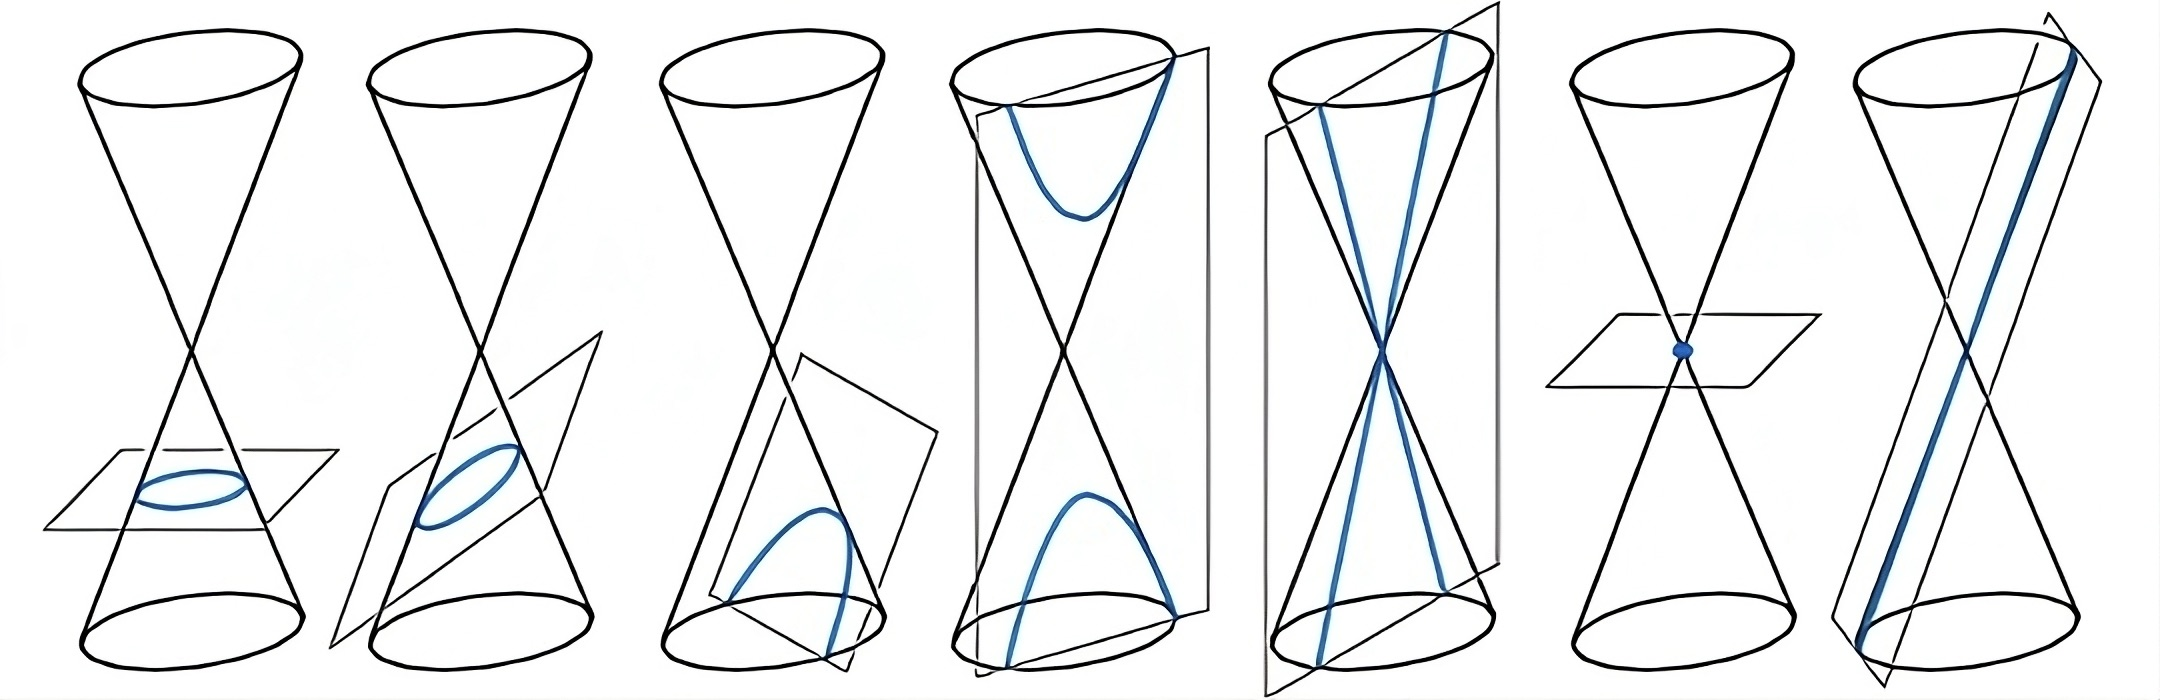
\includegraphics[width=350pt,height=100pt]{media/kegelschnitte.jpeg}};

    \draw (120,130) node [anchor=north west][inner sep=0.75pt]   [align=left] {Kreis};
    \draw (175,130) node [anchor=north west][inner sep=0.75pt]   [align=left] {Ellipse};
    \draw (235,130) node [anchor=north west][inner sep=0.75pt]   [align=left] {Parabel};
    \draw (300,130) node [anchor=north west][inner sep=0.75pt]   [align=left] {Hyperbel};
    \draw (370,130) node [anchor=north west][inner sep=0.75pt]   [align=left] {Geraden};
    \draw (440,130) node [anchor=north west][inner sep=0.75pt]   [align=left] {Punkt};
    \draw (500,130) node [anchor=north west][inner sep=0.75pt]   [align=left] {Gerade};
    \end{tikzpicture}
\end{figure*}

\vspace{\baselineskip}

Zum Beispiel gibt die quadratische Form \( q(\mathbf{x}) = x_1^2 + 4xy + y^2 \), aus der letzten Woche, einen hyperbolischen Kegelschnitt, wenn wir die quadratische Form bei \( z = 1 \) anschauen. Dies kann einfach in einer Abbildung gesehen werden, ist aber schwer direkt aus der quadratischen Form abzulesen. 

\vspace{2\baselineskip}

\begin{figure*}[h]
    \centering
    \begin{tikzpicture}
        \begin{axis}[
            tick label style={font=\footnotesize},
            width=8cm,
            xmax=8,
            xmin=-8, 
            ymax=8,
            ymin=-8, 
            zmin=-50, 
            zmax=150,  
        ]
        \addplot3[
            surf,
            fill=white,
            domain=-5:5,
            domain y=-5:5,
            samples=50,
            z buffer=sort
        ]
        {x^2 + 4*x*y + y^2};
        \addplot3[
            contour gnuplot={
                levels={1},
                labels=false,
                draw color=red
            },
            ultra thick, 
            samples=50,
            domain=-5:5,
            domain y=-5:5,
        ]
        {x^2 + 4*x*y + y^2};
        
        % Add arrow and label
        \node[pin={[pin edge={<-, ultra thick, red}]above right:{\( z=1 \)}}] at (axis cs:5,-1,0) {};
        
        \end{axis}
    \end{tikzpicture}
\end{figure*}

\newpage

Ein besonderer Fall ergibt sich, wenn die Matrix \( A \) diagonal ist, dann sind die Hauptachsen des Kegelschnitts parallel zu den Koordinatenachsen. Ein Kegelschnitt im Hauptachsensystem kann in Normalform geschrieben werden. Die Normalformen aller möglichen Kegelschnitte sind in der folgenden Liste gegeben.

\vspace{\baselineskip}

Rang(\( A \)) = 2:

\begin{equation*}
    \begin{aligned}
        & \frac{x^2}{\alpha^2} + \frac{y^2}{\beta^2} - 1 = 0  \quad \text{Ellipse} \\
        & \frac{x^2}{\alpha^2} - \frac{y^2}{\beta^2} - 1 = 0  \quad \text{Hyperbel} \\
        & \frac{x^2}{\alpha^2} + \frac{y^2}{\beta^2} + 1 = 0  \quad \text{leere Menge} \\
        & x^2 + \beta^2 y^2 = 0 \qquad \ \text{Punkt} \\[0.5em]
        & x^2 - \beta^2 y^2 = 0 \qquad \ \text{Geradenpaar} \\
    \end{aligned}
\end{equation*}
        
Rang(\( A \)) = 1:

\begin{equation*}
    \begin{aligned}
        & x^2 - \gamma y = 0 \qquad \text{Parabel} \\
        & x^2 - \alpha^2 = 0 \qquad \text{paralleles Geradenpaar} \\
        & x^2 + \alpha^2 = 0 \qquad \text{leere Menge} \\
        & x^2 = 0 \qquad \qquad \ \text{Gerade} \\
    \end{aligned}
\end{equation*}

\subsection{Quadriken}

Im allgemeinen Fall, wenn \( A \in \mathbb{R}^{n \times n} \) und \( n > 2 \) ist, kann die Lösungsmenge der quadratischen Form nicht mehr durch Kegelschnitte beschrieben werden. Im Allgemeinen nennen wir dann die Lösungsmenge einer quadratischen Form eine Quadrik. Für den Fall \( n = 3 \) können wir die resultierenden Quadriken noch grafisch als Flächen 2.\ Grades darstellen. Auch hier können wir die Normalformen der Quadriken in einem Hauptachsensystem finden. Einige Beispiele sind:

\vspace{0.5\baselineskip}

\begin{figure*}[h]
    \centering
    \begin{minipage}{0.32\textwidth}
        \centering
        \begin{tikzpicture}
            \begin{axis}[
                width = 5.5cm
            ]
            \addplot3[surf,
                fill=white,
                samples=30,
                samples y=72,
                domain=-1:1,
                y domain=0:360,
                z buffer=sort]
                ( {cosh(x)*cos(y)}, {cosh(x)*sin(y)}, {sinh(x)} );
            \end{axis}
            \draw (1.8,4.5) node [anchor=center][inner sep=0.75pt]   [align=center] {Hyperboloid};
            \draw (1.8,3.75) node [anchor=center][inner sep=0.75pt]   [align=center] {\( \frac{x^2}{\alpha^2} + \frac{y^2}{\beta^2} - \frac{z^2}{\gamma^2} - 1 = 0 \)};
        \end{tikzpicture}
    \end{minipage}
    \hfill
    \begin{minipage}{0.32\textwidth}
        \centering
        \begin{tikzpicture}
            \begin{axis}[
                width = 5.5cm,
                xmin=-2, xmax=2, 
                ymin=-2, ymax=2,  
            ]
            \addplot3[surf,
                fill=white,
                samples=30,
                samples y=72,
                domain=-1:1,
                y domain=0:360,
                z buffer=sort]
                ({2*x},{cos(y)*sqrt(1-x^2)},{sin(y)*sqrt(1-x^2)});
            \end{axis}
            \draw (1.8,4.5) node [anchor=center][inner sep=0.75pt]   [align=center] {Ellipsoid};
            \draw (1.8,3.75) node [anchor=center][inner sep=0.75pt]   [align=center] {\( \frac{x^2}{\alpha^2} + \frac{y^2}{\beta^2} + \frac{z^2}{\gamma^2} - 1 = 0 \)};
        \end{tikzpicture}
    \end{minipage}
    \hfill
    \begin{minipage}{0.32\textwidth}
        \centering
        \begin{tikzpicture}
            \begin{axis}[
                width = 5.5cm,
                xmin=-2, xmax=2, 
                ymin=-2, ymax=2
            ]
            \addplot3[surf,
                fill=white,
                samples=40,
                samples y=40,
                domain=-1.75:1.75,
                domain y= -1.75:1.75, 
                z buffer=sort]
                {x^2 - y^2};
            \end{axis}
            \draw (1.8,4.5) node [anchor=center][inner sep=0.75pt]   [align=center] {Paraboloid};
            \draw (1.8,3.75) node [anchor=center][inner sep=0.75pt]   [align=center] {\( \frac{x^2}{\alpha^2} - \frac{y^2}{\beta^2} - \gamma z = 0 \)};
        \end{tikzpicture}
    \end{minipage}
\end{figure*}

Aber wie genau bringen wir quadratische Formen in die entsprechende Normalform?

\subsection{Hauptachsentransformation}

Bei einer Hauptachsentransformation wird ein Kegelschnitt bzw.\ eine Quadrik in die entsprechende Normalform gebracht. Betrachten wir dieses Verfahren an einem Beispiel. 

\vspace{1\baselineskip}

Aufgabe aus der Prüfung Winter 2018. 
\begin{itemize}
    \item Gegeben sei die quadratische Form 

    \begin{equation*}
        q: \mathbb{R}^2 \to \mathbb{R}, \mapsto q(\mathbf{x})=-x_1^2+4x_1x_2-x_2^2.
    \end{equation*}

    Ein Kegelschnitt \( Q \) ist gegeben durch 

    \begin{equation*}
        q(\mathbf{x}) + a^\top \mathbf{x} = 0, \ \text{wobei} \ a^\top = \begin{pmatrix} 6 & -6 \end{pmatrix}.
    \end{equation*}

    Bringen Sie den Kegelschnitt durch eine Hauptachsentransformation \( x = Ty \) und eine Translation auf Normalform, und geben Sie dabei auch \( T \) explizit an. 

\end{itemize}

Betrachten wir zunächst einmal die gegebene quadratische Form \( q(\mathbf{x}) \). Diese lässt sich im 3D Raum darstellen und kann durch eine symmetrische Matrix \( A \in \mathbb{R}^{2 \times 2} \) beschreiben werden. 

\begin{figure*}[h]
    \centering
    \begin{minipage}{0.32\textwidth}
        \centering
        \begin{equation*}
            A = \begin{pmatrix} -1 & 2 \\ 2 & -1 \end{pmatrix}
        \end{equation*}
        \begin{equation*}
            q(\mathbf{x}) = \mathbf{x}^\top A \  \mathbf{x} 
        \end{equation*}
    \end{minipage}
    \begin{minipage}{0.45\textwidth}
        \begin{tikzpicture}
                \begin{axis}[
                    xlabel={$x_1$},
                    ylabel={$x_2$},
                    tick label style={font=\footnotesize},
                    width=6.5cm,
                    xmax=8,
                    xmin=-8, 
                    ymax=8,
                    ymin=-8, 
                    zmin=-150, 
                    zmax=50,  
                ]
                \addplot3[
                    surf,
                    fill=white,
                    domain=-5:5,
                    domain y=-5:5,
                    samples=40,
                    z buffer=sort
                ]
                {-x^2 + 4*x*y - y^2};
            \end{axis}
        \end{tikzpicture}
    \end{minipage}
\end{figure*}

Der Kegelschnitt \( Q \) beschreibt die Schnittmenge von \( q(\mathbf{x}) \) mit einer Ebene. In 2 Dimensionen lässt sich die Schnittmenge wie folgt darstellen. 

\begin{figure*}[h]
    \centering
    \begin{tikzpicture}[x=0.75pt,y=0.75pt]
        \begin{axis}[
                width = 6cm,
                axis lines = middle,
                xlabel = {\(x_1\)},
                ylabel = {\(x_2\)},
                xlabel style={below right},
                ylabel style={above left}, 
                xmin=-7, xmax=7,
                ymin=-7, ymax=7,
                axis equal,
                xtick=\empty,
                ytick=\empty,
            ]
            \addplot [
                domain=-7:7, 
                samples=50, 
                color=red,
                thick, 
            ]
            {-sqrt(3) * sqrt(x^2 - 2*x + 3) + 2*x - 3};
            \addplot [
                domain=-7:7, 
                samples=50, 
                color=red,
                thick, 
            ]
            {sqrt(3) * sqrt(x^2 - 2*x + 3) + 2*x - 3};
        \end{axis}
        \draw (70,-20) node [anchor=center][inner sep=0.75pt]   [align=center] {\( Q(\mathbf{x}): -x_1^2 + 4x_1x_2 -x_2^2 + 6x_1 - 6x_2 = 0 \)};
    \end{tikzpicture}
\end{figure*}

Zuerst rotieren wir den Kegelschnitt damit die Hauptachsen mit den Koordinatenachsen übereinstimmen. Dazu führen wir einen Basiswechsel \( x = Ty \) durch. In der neuen Basis muss die Matrix \( A \) eine Diagonalmatrix sein. Demnach muss \( A \) diagonalisiert werden. Die dafür benötigten Eigenwerte und Eigenvektoren sind mit 

\begin{equation*}
    \lambda_1 = -3, \quad v_1 = \begin{pmatrix} 1 \\ -1 \end{pmatrix}, \quad \lambda_2 = 1, \quad v_2 = \begin{pmatrix} 1 \\ 1 \end{pmatrix},
\end{equation*}

gegeben. Da wir den Kegelschnitt nur rotieren wollen, ohne seine Form zu verändern, müssen wir unsere Transformationsmatrix \( T \) orthogonal wählen. Dadurch ergibt sich 

\begin{equation*}
    T = \frac{1}{\sqrt{2}} \begin{pmatrix}
        1 & 1 \\
        -1 & 1
    \end{pmatrix}.
\end{equation*}

Nun können wir die Koordinatentransformation durchführen und den Kegelschnitt in der neuen Basis ausdrücken. Per Definition ist \( q(\mathbf{x}) = \mathbf{x}^\top A \mathbf{x} \) wodurch wir \( Q \) umschreiben können.

\begin{equation*}
    Q: q(\mathbf{x}) + a^\top \mathbf{x} = \mathbf{x}^\top A \ \mathbf{x} + a^\top \mathbf{x} = 0
\end{equation*}

Nun setzen wir \( \mathbf{x} = T\mathbf{y} \) ein und erhalten

\begin{equation*}
    \mathbf{x}^\top A \ \mathbf{x} + a^\top \mathbf{x} = \underbrace{(T \mathbf{y})^\top A  \ (T \mathbf{y})}_{\mathbf{y}^\top T^\top A \ T \mathbf{y}} + a^\top T \mathbf{y} = 0
\end{equation*}

Da wir die Matrix \( A \) diagonalisieren und \( T \) orthogonal ist, gilt \( T^\top A \ T = D \). Der Kegelschnitt vereinfacht sich weiterhin zu 

\begin{equation*}
    \mathbf{y}^\top D \ \mathbf{y} + a^\top T \mathbf{y} = -3y_1^2 + y_2^2 + 6 \sqrt{2} y_1 = 0.
\end{equation*}

Was grafisch, wie erwartet, eine Rotation des Kegelschnitts darstellt.
    
\begin{figure*}[h]
    \centering
    \begin{tikzpicture}[x=0.75pt,y=0.75pt]
        \begin{axis}[
                width = 6cm,
                axis lines = middle,
                xlabel = {\(y_1\)},
                ylabel = {\(y_2\)},
                xlabel style={below right},
                ylabel style={above left}, 
                xmin=-7, xmax=7,
                ymin=-7, ymax=7,
                axis equal,
                xtick=\empty,
                ytick=\empty,
            ]
            \addplot [
                domain=-7:0, 
                samples=50, 
                color=red,
                thick, 
            ]
            { -sqrt(3) * sqrt(x^2 - 2 * sqrt(2) * x)};
            \addplot [
                domain=2.8284:7, 
                samples=50, 
                color=red,
                thick, 
            ]
            { -sqrt(3) * sqrt(x^2 - 2 * sqrt(2) * x)};
            \addplot [
                domain=2.8284:7, 
                samples=50, 
                color=red,
                thick, 
            ]
            { sqrt(3) * sqrt(x^2 - 2 * sqrt(2) * x)};
            \addplot [
                domain=-7:0, 
                samples=50, 
                color=red,
                thick, 
            ]
            { sqrt(3) * sqrt(x^2 - 2 * sqrt(2) * x)};
        \end{axis}
        \draw (70,-20) node [anchor=center][inner sep=0.75pt]   [align=center] {\( Q(\mathbf{y}): -3y_1^2 + y_2^2 + 6 \sqrt{2} y_1 = 0 \)};
    \end{tikzpicture}
\end{figure*}

Um die Normalform zu erhalten, müssen wir nur noch, durch eine Translation, den \( y_1-\)Term loswerden. Dafür ergänzen wir quadratisch und erhalten

\begin{equation*}
    \begin{aligned}
        0 = & -3y_1^2 + y_2^2 + 6 \sqrt{2} y_1 \\[0.5em]
        = & -3 \left( y_1^2 - 2\sqrt{2} y_1 \right) + y_2^2 \\[0.5em]
        = & -3 \left( \left(y_1 - \sqrt{2}\right)^2 + 2 \right) + y_2^2 \\[0.5em]
        = & -3 \left(y_1 - \sqrt{2}\right)^2 + y_2^2 + 6.
    \end{aligned}
\end{equation*}

Nun wird eine Translation \( \mathbf{z} = \mathbf{y} + \mathbf{c} \) durchgeführt, wobei der Vektor \( \mathbf{c} \) die Verschiebung in \( y_1 \) Richtung korrigiert. In diesem Fall gilt

\begin{equation*}
    \mathbf{z} = \mathbf{y} + \mathbf{c} = \mathbf{y} + \begin{pmatrix} - \sqrt{2} \\ 0 \end{pmatrix}.
\end{equation*}

Durch einsetzten erhalten wir die Normalform

\begin{equation*}
    \begin{aligned}
        -3z_1^2 + z_2^2 + 6 = 0 \\[0.5em]
        \frac{z_1^2}{2} - \frac{z_2^2}{6} = 1.
    \end{aligned}
\end{equation*}

In der Normalform sehen wir nun eindeutig, dass es sich bei dem Kegelschnitt um eine Hyperbel handelt. Grafisch sieht die Normalform wie folgt aus.

\begin{figure*}[h]
    \centering
    \begin{tikzpicture}[x=0.75pt,y=0.75pt]
        \begin{axis}[
                width = 6cm,
                axis lines = middle,
                xlabel = {\(z_1\)},
                ylabel = {\(z_2\)},
                xlabel style={below right},
                ylabel style={above left}, 
                xmin=-7, xmax=7,
                ymin=-7, ymax=7,
                axis equal,
                xtick=\empty,
                ytick=\empty,
            ]
            \addplot [
                domain=-7:-1.414214, 
                samples=50, 
                color=red,
                thick, 
            ]
            { -sqrt(3) * sqrt(x^2 - 2)};
            \addplot [
                domain=1.414214:7, 
                samples=50, 
                color=red,
                thick, 
            ]
            { -sqrt(3) * sqrt(x^2 - 2)};
            \addplot [
                domain=-7:-1.414214, 
                samples=50, 
                color=red,
                thick, 
            ]
            { sqrt(3) * sqrt(x^2 - 2)};
            \addplot [
                domain=1.414214:7, 
                samples=50, 
                color=red,
                thick, 
            ]
            { sqrt(3) * sqrt(x^2 - 2)};
        \end{axis}
        \draw (70,-20) node [anchor=center][inner sep=0.75pt]   [align=center] {\( Q(\mathbf{z}): \frac{z_1^2}{2} - \frac{z_2^2}{6} - 1  = 0 \)};
    \end{tikzpicture}
\end{figure*}

Wenn wir nun alle Formen vergleichen, ist zu erkennen, dass die Normalform am einfachsten zu interpretieren ist. 

\begin{equation*}
    \begin{aligned}
        Q : & -x_1^2 + 4x_1x_2 - x_2^2 + 6x_1 - 6x_2 = 0 \\[0.5em]
        & -3y_1^2 + y_2^2 + 6\sqrt{2}y_1 = 0 \\[0.5em]
        & \frac{z_1^2}{2} - \frac{z_2^2}{6} - 1 = 0.
    \end{aligned}
\end{equation*}
    \setcounter{section}{8}
\section{Methode der Kleinsten Quadrate und QR-Zerlegung}

\subsection{Methode der kleinsten Quadrate}

Die Methode der kleinsten Quadrate wird immer dann angewendet, wenn wir eine möglichst \textit{gute} Lösung für ein überbestimmtes Gleichungssystem \( Ax = c\) finden wollen, für welches es keine eindeutige Lösung gibt. Ein Gleichungssystem ist überbestimmt, wenn es mehr Gleichungen als Unbekannte hat. Für die Matrix \( A \in \mathbb{R}^{m \times n} \) gilt dann \(m > n \). In realen Anwendungen sind Gleichungssysteme sehr oft Überbestimmt, weswegen es wichtig ist für solche Systeme möglichst \textit{gute} Lösungen zu finden. Was dabei eine \textit{gute} Lösung ausmacht, betrachten wir im folgenden Beispiel. 

\vspace{1\baselineskip}

Bei einer Umfrage werden Menschen bezüglich Körpergrösse und Schuhgrösse befragt. Wir wollen einen Zusammenhang zwischen Körpergrösse und Schuhgrösse finden damit wir nachher basierend auf der Schuhgrösse eine Schätzung für die Körpergrösse machen können. Wir suchen also eine Gleichung der Form

\begin{figure*}[h]
    \centering
    \begin{minipage}
        {0.5\textwidth}
        \begin{equation*}
            \text{Körpergrösse} = x_1\cdot \text{Schuhgrösse} + x_2, \quad (\ddagger)
        \end{equation*}        
    \end{minipage}
    \hfill
    \begin{minipage}
        {0.45\textwidth}
        \centering
        \tikzsetnextfilename{kleinste_quadrate_schuhe_01}
        \begin{tikzpicture}
            \begin{axis}[
                width = 5cm,
                axis lines = middle,
                xlabel = {\text{Schuhgrösse}},
                ylabel = {\text{Körpergrösse}},
                xlabel style={below right},
                ylabel style={above}, 
                xmin=0, xmax=10,
                ymin=0, ymax=10,
                axis equal,
                xtick=\empty,
                ytick=\empty,
            ]
            \addplot [
                domain=0:9.5, 
                samples=5, 
                color=red,
                thick, 
            ]
            { 0.5*x +1 };
            % \node[pin={[pin edge={<-, thick, black}]right:{\( b \)}}] at (axis cs:0,1,0) {};
            \end{axis}
        \end{tikzpicture}
    \end{minipage}
\end{figure*}
    


wobei die Koeffizienten \( x_1, x_2\) unbekannt sind und experimentell durch eine Umfrage ermittelt werden. In einer Umfrage werden nun 8 Menschen befragt, wodurch wir für zwei Unbekannte \( x_1\) und \( x_2\), 8 Gleichungen erhalten. Wir werden also keine eindeutige Lösung für \( x_1\) und \( x_2\) finden können. Wie wählen wir nun die besten Werte für \( x_1\) und \( x_2\) damit die Gleichung \( (\ddagger) \) möglichst gut die Realität repräsentiert? Betrachten wir zunächst die Werte der Umfrage. Aus einer Tabelle mit allen Umfragewerten können wir das überstimmte LGS \( Ax = c \) aufstellen. 

\vspace{1\baselineskip}

\begin{minipage}
    {0.5\textwidth}
    \centering
        \begin{tabular}{|c|c|}
            \hline
            Schuhgrösse & Körpergrösse \\
            \hline
            41 & 172 \\
            45 & 190 \\
            42 & 180 \\
            43 & 183 \\
            43 & 178 \\
            38 & 163 \\
            44 & 180 \\
            40 & 178 \\
            \hline
        \end{tabular}
\end{minipage}
\hfill
\begin{minipage}
    {0.45\textwidth}
    \centering
    \begin{equation*}
        \begin{aligned}
            172 &= x_1\cdot 41 + x_2\\
            190 &= x_1\cdot 45 + x_2\\
            180 &= x_1\cdot 42 + x_2\\
            183 &= x_1\cdot 43 + x_2\\
            178 &= x_1\cdot 43 + x_2\\
            163 &= x_1\cdot 38 + x_2\\
            180 &= x_1\cdot 44 + x_2\\
            178 &= x_1\cdot 40 + x_2\\
        \end{aligned}
    \end{equation*}
\end{minipage}

\vspace{1\baselineskip}

Die Matrix \( A \in \mathbb{R}^{8 \times 2} \) und der Vektor \( c \in \mathbb{R}^{8 \times 1} \) sind dann wie folgt definiert:

\begin{equation*}
    A = \begin{pmatrix}
        41 & 1 \\
        45 & 1 \\
        \vdots & \vdots \\
        40 & 1 \\
    \end{pmatrix}, \quad
    c = \begin{pmatrix}
        172 \\ 190 \\ \vdots \\ 178
    \end{pmatrix}.
\end{equation*}


\vspace{1\baselineskip}

Wir können nun alle Messwerte in einem Koordinatensystem auftragen um zu sehen, wie der Zusammenhang zwischen Schuhgrösse und Körpergrösse aussieht. Als Nächstes wollen wir eine Gerade der Form~\( (\ddagger) \) finden, die möglichst nah an allen Messpunkten ist. Ein Weg dies zu erreichen ist es alle Abstände \( r_i \) von der Geraden zu den Messwerten zu minimieren. 

\vspace{1\baselineskip}

\begin{figure*}[h]
    \centering
    \begin{minipage}
        {0.7\textwidth}
        \centering
        \tikzsetnextfilename{kleinste_quadrate_schuhe_02}
        \begin{tikzpicture}
            \begin{axis}[
                width = 8cm,
                axis lines = middle,
                xlabel = {\text{Schuhgrösse}},
                ylabel = {\text{Körpergrösse}},
                xlabel style={below right},
                ylabel style={above}, 
                xmin=37, xmax=47,
                ymin=155, ymax=195,
            ]
                \addplot[
                    only marks,
                    mark=*,
                    color=black
                ] coordinates {
                    (41,172)
                    (45,190)
                    (42,180)
                    (43,183)
                    (43,178)
                    (38,163)    
                    (44,180)
                    (40,178)
                };
                \addplot[
                    domain=37:46, 
                    samples=5, 
                    color=red,
                    thick, 
                    dotted,
                    opacity =0.5,
                ]
                { 3.083*x +48.5 };
                \addplot[
                    color=orange, 
                    thick       
                ] coordinates {
                    (40,178)   
                    (40, 3.083*40 +48.5 )   
                };
                \addplot[
                    color=orange, 
                    thick       
                ] coordinates {
                    (41,172)   
                    (41, 3.083*41 +48.5 )   
                };
                \addplot[
                    color=orange, 
                    thick       
                ] coordinates {
                    (42,180)   
                    (42, 3.083*42 +48.5 )   
                };
                \addplot[
                    color=orange, 
                    thick       
                ] coordinates {
                    (43,183)   
                    (43, 3.083*43 +48.5 )   
                };
                \addplot[
                    color=orange, 
                    thick       
                ] coordinates {
                    (43,178)   
                    (43, 3.083*43 +48.5 )   
                };
                \addplot[
                    color=orange, 
                    thick       
                ] coordinates {
                    (38,163)   
                    (38, 3.083*38 +48.5 )   
                };
                \addplot[
                    color=orange, 
                    thick       
                ] coordinates {
                    (44,180)   
                    (44, 3.083*44 +48.5 )   
                };
                \addplot[
                    color=orange, 
                    thick       
                ] coordinates {
                    (45,190)   
                    (45, 3.083*45 +48.5 )   
                };
                \node[pin={[pin edge={<-, thick, black}]left:{\( r_i \)}}] at (axis cs:40,175,0) {};
            \end{axis}
        \end{tikzpicture}
    \end{minipage}    
    \hfill
    \begin{minipage}
        {0.29\textwidth}
        \centering
        \begin{equation*}
            \begin{aligned}
                r_1 &= (x_1\cdot 41 + x_2) - 172 \\
                r_2 &= (x_1\cdot 45 + x_2) - 190 \\
                r_3 &= (x_1\cdot 42 + x_2) - 180 \\
                r_4 &= (x_1\cdot 43 + x_2) - 183 \\
                r_5 &= (x_1\cdot 43 + x_2) - 178 \\
                r_6 &= (x_1\cdot 38 + x_2) - 163 \\
                r_7 &= (x_1\cdot 44 + x_2) - 180 \\
                r_8 &= (x_1\cdot 40 + x_2) - 178 \\
            \end{aligned}
        \end{equation*}
    \end{minipage}
\end{figure*}

Da alle Abstände gleichzeitig minimiert werden sollen, fassen wir alle \( r_i \) im sogenannten Residuenvektor \( r = (r_1, \dots, r_m)^\top \) zusammen und minimieren dann die gesamte Länge von \( r \), das entspricht der quadratischen Minimierung des Fehlers \( r \). Wir suchen also das \( x \) sodass

\begin{equation*}
    \lVert r \rVert_2 = \lVert A x - c \rVert_2,
\end{equation*}

\vspace{0.25\baselineskip}

minimal wird. In unserem Fall suchen wir \( x^{opt} = (x_1^{opt} \ \ \ x_2^{opt})^\top\) welches die Länge von \( r \) minimiert. Aber wie können wir dieses Problem lösen? Betrachten wir dafür ein reduziertes Gleichungssystem mit nur drei Gleichungen und zwei Unbekannten, dafür nehmen wir einfach die ersten drei Messwerte von oben. 

\begin{equation*}
    \begin{aligned}
        x_1\cdot 41 + x_2&= 172 \\
        x_1\cdot 45 + x_2&= 190 \\
        x_1\cdot 42 + x_2&= 180 \\
    \end{aligned} \qquad \rightarrow \qquad
    \begin{aligned}
        \underbrace{
        \begin{pmatrix}
            41 & 1 \\
            45 & 1 \\
            42 & 1 \\
        \end{pmatrix}}_{A}
        \begin{pmatrix}
            x_1\\ x_2
        \end{pmatrix}
        =
        \underbrace{
        \begin{pmatrix}
            172 \\ 190 \\ 180
        \end{pmatrix}}_{c} \\
    \end{aligned}
\end{equation*}

Genau wie oben ist dieses LGS überbestimmt und in dieser Form nicht exakt lösbar. Grafisch können wir uns das Problem wie folgt vorstellen. 

\newpage

\begin{figure*}[h]
    \centering
    \tikzsetnextfilename{kleinste_quadrate_schuhe_03}
    \begin{tikzpicture}[x=0.75pt,y=0.75pt,yscale=-1,xscale=1]
        %uncomment if require: \path (0,387); %set diagram left start at 0, and has height of 387
        %Straight Lines [id:da7205339018057622] 
        \draw    (200,280) -- (200,23) ;
        \draw [shift={(200,20)}, rotate = 90] [fill={rgb, 255:red, 0; green, 0; blue, 0 }  ][line width=0.08]  [draw opacity=0] (5.36,-2.57) -- (0,0) -- (5.36,2.57) -- (3.56,0) -- cycle    ;
        %Straight Lines [id:da2519180835664382] 
        \draw    (170,160) -- (347.5,278.34) ;
        \draw [shift={(350,280)}, rotate = 213.69] [fill={rgb, 255:red, 0; green, 0; blue, 0 }  ][line width=0.08]  [draw opacity=0] (5.36,-2.57) -- (0,0) -- (5.36,2.57) -- (3.56,0) -- cycle    ;
        %Straight Lines [id:da9037439858367798] 
        \draw    (170,190) -- (407.15,110.95) ;
        \draw [shift={(410,110)}, rotate = 161.57] [fill={rgb, 255:red, 0; green, 0; blue, 0 }  ][line width=0.08]  [draw opacity=0] (5.36,-2.57) -- (0,0) -- (5.36,2.57) -- (3.56,0) -- cycle    ;
        %Straight Lines [id:da43986582741717895] 
        \draw [color={rgb, 255:red, 126; green, 211; blue, 33 }  ,draw opacity=1 ][line width=1.5]    (200,180) -- (306.14,208.95) ;
        \draw [shift={(310,210)}, rotate = 195.26] [fill={rgb, 255:red, 126; green, 211; blue, 33 }  ,fill opacity=1 ][line width=0.08]  [draw opacity=0] (6.43,-3.09) -- (0,0) -- (6.43,3.09) -- (4.27,0) -- cycle    ;
        %Straight Lines [id:da8398239923702847] 
        \draw [color={rgb, 255:red, 126; green, 211; blue, 33 }  ,draw opacity=1 ][line width=1.5]    (200,180) -- (256.93,132.56) ;
        \draw [shift={(260,130)}, rotate = 140.19] [fill={rgb, 255:red, 126; green, 211; blue, 33 }  ,fill opacity=1 ][line width=0.08]  [draw opacity=0] (6.43,-3.09) -- (0,0) -- (6.43,3.09) -- (4.27,0) -- cycle    ;
        %Shape: Polygon [id:ds9350103434885011] 
        \draw  [color={rgb, 255:red, 126; green, 211; blue, 33 }  ,draw opacity=0.75 ][fill={rgb, 255:red, 126; green, 211; blue, 33 }  ,fill opacity=0.25 ][dash pattern={on 4.5pt off 4.5pt}] (260,130) -- (200,180) -- (310,210) -- (370,160) -- (370,160) -- cycle ;
        % %Curve Lines [id:da7687484645278241] 
        % \draw [color={rgb, 255:red, 126; green, 211; blue, 33 }  ,draw opacity=1 ]   (380,170) .. controls (359.31,185.8) and (354.46,179.81) .. (351.17,172.66) ;
        % \draw [shift={(350,170)}, rotate = 66.37] [fill={rgb, 255:red, 126; green, 211; blue, 33 }  ,fill opacity=1 ][line width=0.08]  [draw opacity=0] (5.36,-2.57) -- (0,0) -- (5.36,2.57) -- (3.56,0) -- cycle    ;
        %Straight Lines [id:da14079628618044737] 
        \draw [color={rgb, 255:red, 208; green, 2; blue, 27 }  ,draw opacity=1 ][line width=1.5]    (200,180) -- (316.05,160.66) ;
        \draw [shift={(320,160)}, rotate = 170.54] [fill={rgb, 255:red, 208; green, 2; blue, 27 }  ,fill opacity=1 ][line width=0.08]  [draw opacity=0] (6.43,-3.09) -- (0,0) -- (6.43,3.09) -- (4.27,0) -- cycle    ;
        %Straight Lines [id:da38161966038314155] 
        \draw [color={rgb, 255:red, 74; green, 144; blue, 226 }  ,draw opacity=1 ][line width=1.5]    (200,180) -- (316.67,102.22) ;
        \draw [shift={(320,100)}, rotate = 146.31] [fill={rgb, 255:red, 74; green, 144; blue, 226 }  ,fill opacity=1 ][line width=0.08]  [draw opacity=0] (6.43,-3.09) -- (0,0) -- (6.43,3.09) -- (4.27,0) -- cycle    ;
        %Straight Lines [id:da5231184422285943] 
        \draw [color={rgb, 255:red, 245; green, 166; blue, 35 }  ,draw opacity=1 ][line width=1.5]    (320,100) -- (320,156) ;
        \draw [shift={(320,160)}, rotate = 270] [fill={rgb, 255:red, 245; green, 166; blue, 35 }  ,fill opacity=1 ][line width=0.08]  [draw opacity=0] (6.43,-3.09) -- (0,0) -- (6.43,3.09) -- (4.27,0) -- cycle    ;
        %Curve Lines [id:da3839403950250917] 
        \draw [color={rgb, 255:red, 0; green, 0; blue, 0 }  ,draw opacity=1 ]   (360,200) .. controls (333.25,201.94) and (311.79,191.65) .. (291.85,171.86) ;
        \draw [shift={(290,170)}, rotate = 45.69] [fill={rgb, 255:red, 0; green, 0; blue, 0 }  ,fill opacity=1 ][line width=0.08]  [draw opacity=0] (5.36,-2.57) -- (0,0) -- (5.36,2.57) -- (3.56,0) -- cycle    ;
        %Curve Lines [id:da9653910687163929] 
        \draw [color={rgb, 255:red, 0; green, 0; blue, 0 }  ,draw opacity=1 ]   (300,60) .. controls (292.84,78.62) and (289.32,91.32) .. (298.6,107.66) ;
        \draw [shift={(300,110)}, rotate = 237.85] [fill={rgb, 255:red, 0; green, 0; blue, 0 }  ,fill opacity=1 ][line width=0.08]  [draw opacity=0] (5.36,-2.57) -- (0,0) -- (5.36,2.57) -- (3.56,0) -- cycle    ;
        %Curve Lines [id:da8838459359016881] 
        \draw [color={rgb, 255:red, 0; green, 0; blue, 0 }  ,draw opacity=1 ]   (370,90) .. controls (347.44,94.32) and (351.61,115.69) .. (328.97,119.6) ;
        \draw [shift={(326,120)}, rotate = 354.51] [fill={rgb, 255:red, 0; green, 0; blue, 0 }  ,fill opacity=1 ][line width=0.08]  [draw opacity=0] (5.36,-2.57) -- (0,0) -- (5.36,2.57) -- (3.56,0) -- cycle    ;
        % % Text Node
        % \draw (381,161) node [anchor=north west][inner sep=0.75pt]  [color={rgb, 255:red, 126; green, 211; blue, 33 }  ,opacity=1 ] [align=left] {Bild von \( A \)};
        % Text Node
        \draw (309,213) node [anchor=north west][inner sep=0.75pt]  [color={rgb, 255:red, 126; green, 211; blue, 33 }  ,opacity=1 ] [align=left] {\( a^{(1)} \)};
        % Text Node
        \draw (223,112) node [anchor=north west][inner sep=0.75pt]  [color={rgb, 255:red, 126; green, 211; blue, 33 }  ,opacity=1 ] [align=left] {\( a^{(2)} \)};
        % Text Node
        \draw (365,200) node [anchor=west][inner sep=0.75pt]  [color={rgb, 255:red, 0; green, 0; blue, 0 }  ,opacity=1 ] [align=left] {\( A \textcolor{customred}{x^{opt}} \in \textcolor{customgreen}{\text{Bild}A} \) };
        % Text Node
        \draw (270,42) node [anchor=north west][inner sep=0.75pt]  [color={rgb, 255:red, 0; green, 0; blue, 0 }  ,opacity=1 ] [align=left] {\( \textcolor{customblue}{c} \notin \textcolor{customgreen}{\text{Bild}A} \)};
        % Text Node
        \draw (375,90) node [anchor=west][inner sep=0.75pt]  [color={rgb, 255:red, 0; green, 0; blue, 0 }  ,opacity=1 ] [align=left] {\( \textcolor{customorange}{r} =  A \textcolor{customred}{x^{opt}} - \textcolor{customblue}{c} \)};
        % Text Node
        \draw (200,282) node [anchor=north][inner sep=0.75pt]  [font=\scriptsize,color={rgb, 255:red, 0; green, 0; blue, 0 }  ,opacity=1 ] [align=center] {nicht Massstäblich};
    \end{tikzpicture}
\end{figure*}

Der Vektor \( x^{opt} \) repräsentiert hier die optimale Lösung, welche den kürzesten Residuenvektor \( r \) hat und im Bild von \( A \) liegt. Grafisch können wir hier auch sehen, dass der Vektor \( r \) minimal ist, wenn er orthogonal zum \( \text{Bild}A \) ist. Für die optimale Lösung muss also gelten:

\begin{equation*}
    \underbrace{A y}_{\text{Bild}A} \ \perp \ r \ , \quad \forall y \in \mathbb{R}^n.
\end{equation*}

Mit dem Skalarprodukt können wir das umformulieren zu

\begin{equation*}
    \langle A  y, r \rangle = 0,
\end{equation*}

\begin{equation*}
    (A  y)^\top  r = 0.
\end{equation*}

Nun können wir unsere Definition für \( r \) einsetzen

\begin{equation*}
    y^\top A^\top \left( A x^{opt} -c \right) = 0, 
\end{equation*}

und alles ausmultiplizieren

\begin{equation*}
    y^\top A^\top A x^{opt} - y^\top A^\top c  = 0.
\end{equation*}

Schliesslich können wir noch umstellen und nach \( x^{opt} \) auflösen

\begin{equation*}
    A^\top c = A^\top A x^{opt},
\end{equation*}

\begin{equation*}
    (A^\top A)^{-1} A^\top c = x^{opt}.
\end{equation*}

Dieser Ausdruck gibt uns nun die optimale Lösung, indem der quadratische Fehler (Länge des Residuenvektors) minimiert wird. Oft wollen wir jedoch nicht die inverse von \( A^\top A \) berechnen und können alternativ das folgende LGS lösen

\begin{equation*}
    A^\top A x^{opt} = A^\top c.
\end{equation*}

\begin{tcolorbox}[colback=gray!30, colframe=gray!80, title=Kleinste Quadrate]
    Wir wollen die optimale Lösung \( x^{opt} \) finden welche den quadratischen Fehler \( \lVert r \rVert_2 = \lVert A x - c \rVert_2 \) minimiert. Oft ist das LGS schon in der Form \( Ax - c = r \) gegeben. 
    \begin{enumerate}
        \item Bestimme \( A \) und \( c \)
        \item Berechne \( A^\top A \) und \( A^\top c \)
        \item Löse das LGS \( A^\top A x^{opt} = A^\top c \)
    \end{enumerate}
\end{tcolorbox}

\subsection{QR-Zerlegung}

Bei der QR-Zerlegung werden wir eine Matrix \( A \in \mathbb{R}^{m \times n} \) in das Produkt einer orthogonalen Matrix \( Q \in \mathbb{R}^{m \times m} \) und einer oberen Dreiecksmatrix \( R \in \mathbb{R}^{m \times n} \) zerlegen. Es gilt dann 

\vspace{1\baselineskip}

\begin{figure}[h]
    \tikzsetnextfilename{qr_zerlegung_01}
    \centering
    \begin{tikzpicture}[x=0.75pt,y=0.75pt,yscale=-1,xscale=1]
        %uncomment if require: \path (0,300); %set diagram left start at 0, and has height of 300
        
        %Shape: Rectangle [id:dp842902263884775] 
        \draw   (170,50) -- (230,50) -- (230,140) -- (170,140) -- cycle ;
        %Shape: Rectangle [id:dp1365802461569866] 
        \draw   (300,50) -- (390,50) -- (390,140) -- (300,140) -- cycle ;
        %Shape: Rectangle [id:dp06826642370754088] 
        \draw   (440,50) -- (500,50) -- (500,140) -- (440,140) -- cycle ;
        %Straight Lines [id:da11387891999511401] 
        \draw  [dash pattern={on 4.5pt off 4.5pt}]  (450,60) -- (490,100) ;
        
        % Text Node
        \draw (141,90) node [anchor=north west][inner sep=0.75pt]   [align=left] {$\displaystyle m$};
        % Text Node
        \draw (191,147) node [anchor=north west][inner sep=0.75pt]   [align=left] {$\displaystyle n$};
        % Text Node
        \draw (241,90) node [anchor=north west][inner sep=0.75pt]   [align=left] {$\displaystyle =$};
        % Text Node
        \draw (271,90) node [anchor=north west][inner sep=0.75pt]   [align=left] {$\displaystyle m$};
        % Text Node
        \draw (341,147) node [anchor=north west][inner sep=0.75pt]   [align=left] {$\displaystyle m$};
        % Text Node
        \draw (401,90) node [anchor=north west][inner sep=0.75pt]   [align=left] {$\displaystyle \cdot $};
        % Text Node
        \draw (191,12) node [anchor=north west][inner sep=0.75pt]   [align=left] {$\displaystyle A$};
        % Text Node
        \draw (341,12) node [anchor=north west][inner sep=0.75pt]   [align=left] {$\displaystyle Q$};
        % Text Node
        \draw (411,90) node [anchor=north west][inner sep=0.75pt]   [align=left] {$\displaystyle m$};
        % Text Node
        \draw (461,147) node [anchor=north west][inner sep=0.75pt]   [align=left] {$\displaystyle n$};
        % Text Node
        \draw (461,12) node [anchor=north west][inner sep=0.75pt]   [align=left] {$\displaystyle R$};
        % Text Node
        \draw (241,16) node [anchor=north west][inner sep=0.75pt]   [align=left] {$\displaystyle =$};
        % Text Node
        \draw (401,16) node [anchor=north west][inner sep=0.75pt]   [align=left] {$\displaystyle \cdot $};
        % Text Node
        \draw (451,90) node [anchor=north west][inner sep=0.75pt]   [align=left] {$\displaystyle 0$};
        % Text Node
        \draw (481,118) node [anchor=north west][inner sep=0.75pt]   [align=left] {$\displaystyle 0$};
        % Text Node
        \draw (451,118) node [anchor=north west][inner sep=0.75pt]   [align=left] {$\displaystyle 0$};
    \end{tikzpicture}
\end{figure}    

Später können wir die QR-Zerlegung als ein alternatives Lösungsverfahren der kleinsten Quadrate verwenden. Um die QR-Zerlegung zu berechnen, müssen einige Schritte befolgt werden. Betrachten wir das Ganze an einem Beispiel.

\vspace{1\baselineskip}

Wir suchen nun \( Q \) und \( R \) sodass für die Matrix 

\begin{equation*}
    A = \begin{pmatrix}
        1 & 0 \\
        0 & 1 \\
        1 & 1 \\
    \end{pmatrix},
\end{equation*}

gilt \( A = QR \). Dafür eliminieren wir schrittweise alle Elemente \( a_{ij} \) unterhalb der Hauptdiagonalen von \( A \). In unserem fall beginnen wir mit dem Eintrag \( a_{31} \). Zuerst notieren wir die Werte für \( i, j \) und die Einträge \( a_{jj}, \ a_{ij} \) 

\begin{equation*}
    i = 3, \ j = 1. 
\end{equation*}

\begin{equation*}
    a_{jj} = 1, \ a_{ij} = 1.
\end{equation*}

Anschliessend berechnen wir den Wert einer Zwischenvariable \( \omega \) gegeben durch

\begin{equation*}
    \omega = \sqrt{a_{jj}^2 + a_{ij}^2} = \sqrt{1^2 + 1^2} = \sqrt{2}.
\end{equation*}

Als Nächstes suchen wir eine Rotationsmatrix \( Q^{\prime \top} \). Dafür fangen wir mit einer Identitätsmatrix \( I \in \mathbb{R}^{m \times m} \) an und füllen die Einträge wie folgt ein

\begin{equation*}
    i_{ii} = \cos(\alpha), \ i_{ij} = -\sin(\alpha), \ i_{ji} = \sin(\alpha), \ i_{jj} = \cos(\alpha).
\end{equation*}

Wobei die spezifischen Werte für cos und sin durch das \( \omega \) gegeben sind

\begin{equation*}
    \sin(\alpha) = \frac{a_{ij}}{\omega} = \frac{1}{\sqrt{2}}, \quad \cos(\alpha) = \frac{a_{jj}}{\omega} = \frac{1}{\sqrt{2}}.
\end{equation*}

In unserem Fall ist \( Q'^\top \) gegeben durch

\begin{equation*}
    Q'^\top = \begin{pmatrix}
        \cos(\alpha) & 0 & \sin(\alpha) \\
        0 & 1 & 0 \\
        - \sin(\alpha) & 0 & \cos(\alpha) \\
    \end{pmatrix} =
    \begin{pmatrix}
        \frac{1}{\sqrt{2}} & 0 & \frac{1}{\sqrt{2}} \\
        0 & 1 & 0 \\
        -\frac{1}{\sqrt{2}} & 0 & \frac{1}{\sqrt{2}} \\
    \end{pmatrix}.
\end{equation*}

Nun Berechnen wir die Matrix \( A' = Q'^\top A \) und überprüfen ob \( A' \) eine obere Dreiecksmatrix ist.

\begin{equation*}
    A' = Q'^\top A = 
    \begin{pmatrix}
        \frac{1}{\sqrt{2}} & 0 & \frac{1}{\sqrt{2}} \\
        0 & 1 & 0 \\
        -\frac{1}{\sqrt{2}} & 0 & \frac{1}{\sqrt{2}} \\
    \end{pmatrix}
    \begin{pmatrix}
        1 & 0 \\
        0 & 1 \\
        1 & 1 \\
    \end{pmatrix} = 
    \begin{pmatrix}
        \sqrt{2} & \frac{1}{\sqrt{2}} \\
        0 & 1 \\
        0 & \frac{1}{\sqrt{2}} \\
    \end{pmatrix}.
\end{equation*}

Falls, wie in unserem Fall, \( A' \) keine obere Dreiecksmatrix ist, wiederholen wir den Prozess und nehmen den nächsten Eintrag unterhalb der Hauptdiagonalen von \( A ^\prime \). Hier wäre das der Eintrag \( a^\prime_{32} \) dadurch werden \( i = 3, j = 2 \). Wir lesen wieder die Einträge \( a'_{ij}, a'_{jj} \) und \( \omega \) ab

\begin{equation*}
    a'_{jj} = 1, \ a'_{ij} = \frac{1}{\sqrt{2}}, \ \omega = \sqrt{\frac{3}{2}}.
\end{equation*}

Weiter konstruieren wir wie oben eine Rotationsmatrix \( Q''^\top \) welche die folgende Form annimmt

\begin{equation*}
    Q''^\top = \begin{pmatrix}
        1 & 0 & 0 \\
        0 & \cos(\alpha) & \sin(\alpha) \\
        0 & -\sin(\alpha) & \cos(\alpha) \\
    \end{pmatrix} =
    \begin{pmatrix}
        1 & 0 & 0 \\
        0 & \frac{\sqrt{2}}{\sqrt{3}} & \frac{1}{\sqrt{3}} \\
        0 & -\frac{1}{\sqrt{3}} & \frac{\sqrt{2}}{\sqrt{3}} \\
    \end{pmatrix},
\end{equation*}

wodurch wir die Matrix \( A'' = Q''^\top A' \) erhalten

\begin{equation*}
    A'' =
    \begin{pmatrix}
        \sqrt{2} & \frac{1}{\sqrt{2}} \\
        0 & \frac{\sqrt{3}}{\sqrt{2}} \\
        0 & 0 \\
    \end{pmatrix}.
\end{equation*}

Nun ist \( A'' \) eine obere Dreiecksmatrix und es gilt \( A'' = R \). Um schliesslich noch die Matrix \( Q \) zu erhalten, multiplizieren wir alle Rotationsmatrizen zusammen 

\begin{equation*}
    Q^\top = Q''^\top Q'^\top.
\end{equation*}

Somit ist die QR-Zerlegung vollendet. Zusammengefasst müssen also folgende Schritte befolgt werden. 

\begin{tcolorbox}[colback=gray!30, colframe=gray!80, title=QR-Zerlegung]
    Bei der QR-Zerlegung Zerlegen wir eine Matrix \( A \in \mathbb{R}^{m \times n} \) in das Produkt einer orthogonalen Matrix \( Q \in \mathbb{R}^{m \times m} \) und einer oberen Dreiecksmatrix \( R \in \mathbb{R}^{m \times n} \). Nach und nach eliminieren wir die Einträge unterhalb der Hauptdiagonalen von \( A \). 
    \begin{enumerate}
        \item Wähle das zu eliminierende Element \( a_{ij} \) unter der Hauptdiagonalen
        \item Notiere die Werte \( i, j, a_{ij}, a_{jj} \)
        \item Berechne \( \omega = \sqrt{a_{ij}^2 + a_{jj}^2} \)
        \item Finde die Rotationsmatrix \( Q'^\top \) basierend auf einer Identitätsmatrix \( I \in \mathbb{R}^{m \times m} \) und setze \( i_{ii} = \cos(\alpha), i_{ij} = -\sin(\alpha), i_{ji} = \sin(\alpha), i_{jj} = \cos(\alpha) \)
        \item Für die Werte von \( \cos(\alpha) \) und \( \sin(\alpha) \) setze \( \sin(\alpha) = \frac{a_{ij}}{\omega}, \cos(\alpha) = \frac{a_{jj}}{\omega} \)
        \item Berechne \( A' = Q'^\top A \)
        \item Überprüfe ob \( A' \) eine obere Dreiecksmatrix ist, falls nicht, wiederhole den Prozess mit dem nächsten Eintrag \( a'_{ij} \) von \( A' \) solange, bis alle Einträge unterhalb der Hauptdiagonalen eliminiert sind
        \item Wenn nach \( k \) Wiederholungen \( A^{(k)} = R \) ist, berechne \( Q^\top = Q^{(k) \top} \cdot ... \cdot Q''^\top \cdot Q'^\top \)
        \item Nun ist \(A = QR\)
    \end{enumerate}
\end{tcolorbox}

\subsection{Kleinste Quadrate mit QR-Zerlegung}

In gewissen Fällen kann es sein das die oben gezeigte Methode zur Lösung von überbestimmten LGS ungenaue Ergebnisse liefert. Vor allem, wenn Sie numerisch mit dem Computer berechnet werden. Oft kann man für eine numerisch stabilere Lösung die QR-Zerlegung verwenden. 

\begin{tcolorbox}[colback=gray!30, colframe=gray!80, title=Kleinste Quadrate mit QR-Zerlegung]
    Ein alternativer Lösungsweg um überbestimmte LGS \( Ax=c\) durch kleinste Quadrate zu lösen. 
    \begin{enumerate}
        \item Bestimme \( A \) und \( c \)
        \item Berechne die QR-Zerlegung \( A = QR \)
        \item Berechne \( d = Q^\top c \)
        \item Löse das LGS \( R_0 x = d_0 \), wobei \( R_0 \) die extrahierte Dreiecksmatrix von \( R \) ist und \( d_0 \) die dazugehörigen oberen Einträge von \( d \)
        \item Die Lösung \( x \) ist die optimale Lösung für \( Ax = c \)
    \end{enumerate}
\end{tcolorbox}
    \setcounter{section}{9}
\section{Lineare Differentialgleichungssysteme}

\subsection{Homogene lineare Differentialgleichungen 1.\ Ordnung mit konstanten Koeffizienten}

Solche Gleichungen sind bereits aus der Analysis bekannt. Allgemein ist eine solche Differentialgleichung gegeben durch

\begin{equation*}
    y'(t)=ay(t), \quad a \in \mathbb{R}.
\end{equation*}

Mit der Lösung

\begin{equation*}
    y(t)= y(0) \ e^{at}.
\end{equation*}

Wobei \( y(0) \) die Anfangsbedingung ist. Ein konkretes Beispiel hierfür ist die Differentialgleichung

\begin{equation*}
    y'(t)=-2y(t),\  y(0) = 3.
\end{equation*}

Die Lösung ist dann gegeben durch 

\begin{figure*}[h]
    \centering
    \begin{minipage}
        {0.5\textwidth}
        \begin{equation*}
            y(t) = y(0) e^{-2t} = 3 e^{-2t}.
        \end{equation*}        
    \end{minipage}
    \hfill
    \begin{minipage}
        {0.45\textwidth}
        \centering
        \tikzsetnextfilename{lin_diff_01}
        \begin{tikzpicture}
            \begin{axis}[
                width = 5cm,
                axis lines = middle,
                xlabel = {t},
                ylabel = {y},
                xlabel style={below right},
                ylabel style={above}, 
                xmin=-0.5, xmax=4.5,
                % ymin=0, ymax=3.5,
                axis equal,
                xtick=\empty,
                ytick=\empty,
            ]
            \addplot [
                domain=-0.25:4, 
                samples=40, 
                color=red,
                thick, 
            ]
            { 3 *exp(-2*x) };
            % \node[pin={[pin edge={<-, thick, black}]right:{\( b \)}}] at (axis cs:0,1,0) {};
            \end{axis}
        \end{tikzpicture}
    \end{minipage}
\end{figure*}

Die Lösungsmenge dieser Differentialgleichung \( \left\{ y \in C^1(\mathbb{R}): y' = ay \right\} \) ist ein 1-D Unterraum von den 1-mal stetig differenzierbaren Funktionen \( C^1(\mathbb{R}) \).

\subsection{Systeme homogener linearer Differentialgleichungen 1.\ Ordnung mit konstanten Koeffizienten}

In der linearen Algebra I haben wir bereits gesehen wie wir Systeme von Gleichungen lösen und manipulieren können. Das geht auch mit Differentialgleichungen. Ein Beispiel dafür wäre zum Beispiel das Gleichungssystem gegeben durch

\vspace{1\baselineskip}

\begin{equation*}
    \left\{ 
        \begin{aligned}
            y_1'(t) &= -2 y_1(t), \quad y_1(0) = 1 \\
            y_2'(t) &= -4 y_2(t), \quad y_2(0) = 3. \\
        \end{aligned}
    \right.
\end{equation*}

\vspace{0.5\baselineskip}

Da beide Gleichungen von unterschiedlichen Variablen abhängen und dadurch unabhängig voneinander sind, nennen wir ein solches System entkoppelt. In einem solchen entkoppelten System können wir die Differentialgleichungen separat voneinander lösen. 

\newpage

\begin{figure*}[h]
    \centering
    \begin{minipage}
        {0.5\textwidth}
        \begin{equation*}
            \textcolor{customblue}{y_1(t)} = y_1(0) e^{-2t} = e^{-2t}
        \end{equation*}        
    \end{minipage}
    \hfill
    \begin{minipage}
        {0.45\textwidth}
        \centering
        \tikzsetnextfilename{lin_diff_02}
        \begin{tikzpicture}
            \begin{axis}[
                width = 5cm,
                axis lines = middle,
                xlabel = {t},
                ylabel = {\( y_1 \)},
                xlabel style={below right},
                ylabel style={above}, 
                xmin=-0.5, xmax=2.5,
                ymin=-0.5, ymax=3.5,
                % axis equal,
                xtick=\empty,
                ytick=\empty,
            ]
            \addplot [
                domain=0:2.25, 
                samples=40, 
                color=blue,
                thick, 
            ]
            { exp(-2*x) };
            % \node[pin={[pin edge={<-, thick, black}]right:{\( b \)}}] at (axis cs:0,1,0) {};
            \end{axis}
        \end{tikzpicture}
    \end{minipage}
\end{figure*}

\begin{figure*}[h]
    \centering
    \begin{minipage}
        {0.5\textwidth}
        \begin{equation*}
            \textcolor{customred}{y_2(t)} = y_2(0) e^{-4t} = 3 e^{-4t}
        \end{equation*}        
    \end{minipage}
    \hfill
    \begin{minipage}
        {0.45\textwidth}
        \centering
        \tikzsetnextfilename{lin_diff_03}
        \begin{tikzpicture}
            \begin{axis}[
                width = 5cm,
                axis lines = middle,
                xlabel = {t},
                ylabel = {\( y_2 \)},
                xlabel style={below right},
                ylabel style={above}, 
                xmin=-0.5, xmax=2.5,
                ymin=-0.5, ymax=3.5,
                % axis equal,
                xtick=\empty,
                ytick=\empty,
            ]
            \addplot [
                domain=0:2.25, 
                samples=40, 
                color=red,
                thick, 
            ]
            { 3 * exp(-4*x) };
            % \node[pin={[pin edge={<-, thick, black}]right:{\( b \)}}] at (axis cs:0,1,0) {};
            \end{axis}
        \end{tikzpicture}
    \end{minipage}
\end{figure*}

Wie bei den herkömmlichen LGS der Form \( Ax = b \), können wir auch dieses System von linearen Differentialgleichungen in Matrixform schreiben bloss, dass die allgemeine Form nun \( y' = Ay \) ist. In unserem Fall ergibt sich

\begin{equation*}
    \begin{pmatrix}
        y_1'(t) \\
        y_2'(t)
    \end{pmatrix} = 
    \begin{pmatrix}
        -2 & 0 \\
        0 & -4
    \end{pmatrix}
    \begin{pmatrix}
        y_1(t) \\
        y_2(t)
    \end{pmatrix},
    \quad \begin{pmatrix}
        y_1(0) \\
        y_2(0)
    \end{pmatrix} = y(0) =
    \begin{pmatrix}
        1 \\
        3
    \end{pmatrix}.
\end{equation*}

\vspace{0.25\baselineskip}

Die Lösung dieses Systems lässt sich dann als Vektor schreiben:

\begin{equation*}
    y(t) = 
    e^{-2t}
    \begin{pmatrix}
        1 \\
        0
    \end{pmatrix} +
    e^{-4t}
    \begin{pmatrix}
        0 \\
        3
    \end{pmatrix}.
\end{equation*}

\vspace{0.25\baselineskip}

Grafisch können wir uns die zusammengesetzte Lösung von \( y_1 \) und \( y_2 \) wie eine Linearkombination vorstellen, bloss das jetzt alles noch von \( t \) abhängt. 

\begin{figure}[h]
    \centering
    \tikzsetnextfilename{lin_diff_04}
    \begin{tikzpicture}[x=0.75pt,y=0.75pt,yscale=-1,xscale=1]
        %Straight Lines [id:da6266944733728231] 
        \draw [color={rgb, 255:red, 208; green, 2; blue, 27 }  ,draw opacity=0.5 ]   (242.33,147.17) -- (242.33,251.17) ;
        %Straight Lines [id:da9473718551797458] 
        \draw [color={rgb, 255:red, 208; green, 2; blue, 27 }  ,draw opacity=0.5 ]   (264.08,162.92) -- (264.08,241.92) ;
        %Straight Lines [id:da3375189209092121] 
        \draw [color={rgb, 255:red, 208; green, 2; blue, 27 }  ,draw opacity=0.5 ]   (286.83,172.42) -- (286.83,233.42) ;
        %Straight Lines [id:da585381201015521] 
        \draw [color={rgb, 255:red, 208; green, 2; blue, 27 }  ,draw opacity=0.5 ]   (308.83,176.42) -- (308.83,224.42) ;
        %Straight Lines [id:da989334182528751] 
        \draw [color={rgb, 255:red, 208; green, 2; blue, 27 }  ,draw opacity=0.5 ]   (331.08,178.42) -- (331.08,215.42) ;
        %Straight Lines [id:da21157481547876977] 
        \draw [color={rgb, 255:red, 208; green, 2; blue, 27 }  ,draw opacity=0.5 ]   (353.33,178.42) -- (353.33,206.42) ;
        %Straight Lines [id:da6750318344383669] 
        \draw [color={rgb, 255:red, 208; green, 2; blue, 27 }  ,draw opacity=0.5 ]   (375.33,175.67) -- (375.33,197.67) ;
        %Straight Lines [id:da07171771142136829] 
        \draw [color={rgb, 255:red, 208; green, 2; blue, 27 }  ,draw opacity=0.5 ]   (397.33,172.67) -- (397.33,188.67) ;
        %Straight Lines [id:da4075047389571379] 
        \draw [color={rgb, 255:red, 208; green, 2; blue, 27 }  ,draw opacity=0.5 ]   (419.83,167.92) -- (419.83,179.92) ;
        %Straight Lines [id:da6591683928404128] 
        \draw [color={rgb, 255:red, 208; green, 2; blue, 27 }  ,draw opacity=0.5 ]   (442,163) -- (442,171) ;
        %Straight Lines [id:da9909465982671221] 
        \draw [color={rgb, 255:red, 74; green, 144; blue, 226 }  ,draw opacity=0.5 ]   (242.33,251.17) -- (286.25,273.25) ;
        %Straight Lines [id:da3756346843414533] 
        \draw [color={rgb, 255:red, 74; green, 144; blue, 226 }  ,draw opacity=0.5 ]   (264.08,241.92) -- (297.08,258.67) ;
        %Straight Lines [id:da9777741491261767] 
        \draw [color={rgb, 255:red, 74; green, 144; blue, 226 }  ,draw opacity=0.5 ]   (286.83,233.42) -- (311.08,245.42) ;
        %Straight Lines [id:da21510571632197606] 
        \draw [color={rgb, 255:red, 74; green, 144; blue, 226 }  ,draw opacity=0.5 ]   (308.83,224.42) -- (327.58,233.67) ;
        %Straight Lines [id:da5494003280478376] 
        \draw [color={rgb, 255:red, 74; green, 144; blue, 226 }  ,draw opacity=0.5 ]   (331.08,215.42) -- (344.83,222.42) ;
        %Straight Lines [id:da8304348712132449] 
        \draw [color={rgb, 255:red, 74; green, 144; blue, 226 }  ,draw opacity=0.5 ]   (353.33,206.42) -- (364.58,212.17) ;
        %Straight Lines [id:da10249677615168695] 
        \draw [color={rgb, 255:red, 74; green, 144; blue, 226 }  ,draw opacity=0.5 ]   (375.33,197.67) -- (384.33,202.17) ;
        %Straight Lines [id:da33625113634117754] 
        \draw [color={rgb, 255:red, 74; green, 144; blue, 226 }  ,draw opacity=0.5 ]   (397.33,188.67) -- (405.08,192.42) ;
        %Straight Lines [id:da4720358563705469] 
        \draw [color={rgb, 255:red, 74; green, 144; blue, 226 }  ,draw opacity=0.5 ]   (419.83,179.92) -- (427.08,183.42) ;
        %Straight Lines [id:da3548721469063173] 
        \draw [color={rgb, 255:red, 74; green, 144; blue, 226 }  ,draw opacity=0.5 ]   (441.83,170.92) -- (449.08,174.42) ;
        %Straight Lines [id:da17981019374494978] 
        \draw    (220,260) -- (467.21,161.11) ;
        \draw [shift={(470,160)}, rotate = 158.2] [fill={rgb, 255:red, 0; green, 0; blue, 0 }  ][line width=0.08]  [draw opacity=0] (5.36,-2.57) -- (0,0) -- (5.36,2.57) -- (3.56,0) -- cycle    ;
        %Curve Lines [id:da2959295993490375] 
        \draw [color={rgb, 255:red, 74; green, 144; blue, 226 }  ,draw opacity=1 ][line width=1.5]    (460,170) .. controls (468.42,171.25) and (288.5,224.5) .. (280,290) ;
        %Curve Lines [id:da9691686052962586] 
        \draw [color={rgb, 255:red, 208; green, 2; blue, 27 }  ,draw opacity=1 ][line width=1.5]    (450,160) .. controls (460,157) and (219.33,238.67) .. (220,80) ;
        %Straight Lines [id:da21487560786590698] 
        \draw [color={rgb, 255:red, 126; green, 211; blue, 33 }  ,draw opacity=1 ] [dash pattern={on 4.5pt off 4.5pt}]  (220,80) -- (280,110) ;
        %Straight Lines [id:da7887659673436868] 
        \draw [color={rgb, 255:red, 126; green, 211; blue, 33 }  ,draw opacity=1 ] [dash pattern={on 4.5pt off 4.5pt}]  (280,290) -- (280,110) ;
        %Straight Lines [id:da09158980326810207] 
        \draw [color={rgb, 255:red, 126; green, 211; blue, 33 }  ,draw opacity=1 ] [dash pattern={on 4.5pt off 4.5pt}]  (344.83,222.42) -- (344.83,188.67) ;
        %Straight Lines [id:da5344220902516645] 
        \draw [color={rgb, 255:red, 126; green, 211; blue, 33 }  ,draw opacity=1 ] [dash pattern={on 4.5pt off 4.5pt}]  (331.08,178.42) -- (345,186) ;
        %Straight Lines [id:da7246234521000464] 
        \draw [color={rgb, 255:red, 126; green, 211; blue, 33 }  ,draw opacity=1 ] [dash pattern={on 4.5pt off 4.5pt}]  (405.08,192.42) -- (404.92,178.5) ;
        %Straight Lines [id:da30101186267489277] 
        \draw [color={rgb, 255:red, 126; green, 211; blue, 33 }  ,draw opacity=1 ] [dash pattern={on 4.5pt off 4.5pt}]  (397.33,172.67) -- (404.92,176.5) ;
        %Curve Lines [id:da25368345747771415] 
        \draw [color={rgb, 255:red, 126; green, 211; blue, 33 }  ,draw opacity=1 ][line width=1.5]    (280,110) .. controls (296.69,248.25) and (429.42,161.75) .. (449,166.5) ;
        %Straight Lines [id:da04224144437602262] 
        \draw [color={rgb, 255:red, 126; green, 211; blue, 33 }  ,draw opacity=1 ][line width=1.5]    (220,260) -- (278.51,113.71) ;
        \draw [shift={(280,110)}, rotate = 111.8] [fill={rgb, 255:red, 126; green, 211; blue, 33 }  ,fill opacity=1 ][line width=0.08]  [draw opacity=0] (8.75,-4.2) -- (0,0) -- (8.75,4.2) -- (5.81,0) -- cycle    ;
        %Straight Lines [id:da6973116866864064] 
        \draw    (220,310) -- (220,53) ;
        \draw [shift={(220,50)}, rotate = 90] [fill={rgb, 255:red, 0; green, 0; blue, 0 }  ][line width=0.08]  [draw opacity=0] (5.36,-2.57) -- (0,0) -- (5.36,2.57) -- (3.56,0) -- cycle    ;
        %Straight Lines [id:da19482417766302107] 
        \draw    (180,240) -- (337.32,318.66) ;
        \draw [shift={(340,320)}, rotate = 206.57] [fill={rgb, 255:red, 0; green, 0; blue, 0 }  ][line width=0.08]  [draw opacity=0] (5.36,-2.57) -- (0,0) -- (5.36,2.57) -- (3.56,0) -- cycle    ;
        %Straight Lines [id:da5500107339514307] 
        \draw [color={rgb, 255:red, 126; green, 211; blue, 33 }  ,draw opacity=1 ] [dash pattern={on 4.5pt off 4.5pt}]  (449.08,174.42) -- (448.92,166.5) ;
        %Straight Lines [id:da1413956810230076] 
        \draw [color={rgb, 255:red, 126; green, 211; blue, 33 }  ,draw opacity=1 ] [dash pattern={on 4.5pt off 4.5pt}]  (442,163) -- (449.58,166.83) ;

        % Text Node
        \draw (342,323) node [anchor=north west][inner sep=0.75pt]   [align=left] {$\displaystyle y_{1}$};
        % Text Node
        \draw (192,41) node [anchor=north west][inner sep=0.75pt]   [align=left] {$\displaystyle y_{2}$};
        % Text Node
        \draw (479,151) node [anchor=north west][inner sep=0.75pt]   [align=left] {$\displaystyle t$};

    \end{tikzpicture}
\end{figure}

Es kann aber auch sein, dass die Differentialgleichungen nicht entkoppelt sind. In dem Fall sind die Gleichungen voneinander abhängig und wir können sie nicht mehr separat lösen. Ein Beispiel dafür wäre das Gleichungssystem

\begin{equation*}
    \left\{ 
        \begin{aligned}
            y_1'(t) &= -4 y_1(t) - y_2(t) \\
            y_2'(t) &= -2 y_1(t) - 3 y_2(t)
        \end{aligned}
    \right. \quad \longrightarrow \quad
    \underbrace{\begin{pmatrix}
        y_1'(t) \\
        y_2'(t)
    \end{pmatrix} =
    \begin{pmatrix}
        -4 & -1 \\
        -2 & -3
    \end{pmatrix}
    \begin{pmatrix}
        y_1(t) \\
        y_2(t)
    \end{pmatrix}}_{\text{nicht direkt lösbar}}, \quad y(0)=
    \begin{pmatrix}
        1 \\
        3
    \end{pmatrix}.
\end{equation*}

Es stellt sich nun die Frage wie wir ein solches System dennoch lösen können. Betrachten wir dafür nochmals genauer die Matrizen \( A_1\) und \( A_2 \) der beiden Systeme.

\begin{equation*}
    A_1 = \begin{pmatrix}
        -2 & 0 \\
        0 & -4
    \end{pmatrix}, \quad
    A_2 = \begin{pmatrix}
        -4 & -1 \\
        -2 & -3
    \end{pmatrix}.
\end{equation*}

Wir erkennen, dass die Matrix \( A_1 \) des entkoppelten Systems diagonal ist. Im Rückschluss können wir also für das zweite System eine Lösung finden, indem wir einen Basiswechsel \( y = Tz \) durchführen und dadurch die Matrix \( A_2 \) diagonalisieren. Wir transformieren also das gesamte Gleichungssystem in die Eigenbasis von \( A_2 \). Dafür benötigen wir die Eigenwerte und Eigenvektoren, welche die Spalten unserer Transformationsmatrix \( T \) bilden.   

\begin{equation*}
    \lambda_1 = -2, \quad \lambda_2 = -5, \quad T = \begin{pmatrix}
        -\frac{1}{2} & 1 \\
        1 & 1
    \end{pmatrix}, \quad T^{-1} = \frac{1}{3} \begin{pmatrix}
        -2 & 2 \\
        2 & 1
    \end{pmatrix}.
\end{equation*}

Nun können wir die Transformation durchführen. 

\begin{equation*}
        \begin{aligned}
            \begin{pmatrix}
                y_1'(t) \\
                y_2'(t)
            \end{pmatrix} &=
            \begin{pmatrix}
                -4 & -1 \\
                -2 & -3
            \end{pmatrix}
            \begin{pmatrix}
                y_1(t) \\
                y_2(t)
            \end{pmatrix} \\[0.5em]
            y(0)&= \begin{pmatrix}
                y_1(0) \\
                y_2(0)
            \end{pmatrix}
            \begin{pmatrix}
                1 \\
                3
            \end{pmatrix} 
        \end{aligned} \quad \xRightarrow{y = Tz} \quad
        \begin{aligned}
            \begin{pmatrix}
                z_1'(t) \\
                z_2'(t)
            \end{pmatrix} &=
            \underbrace{\begin{pmatrix}
                -2 & 0 \\
                0 & -5
            \end{pmatrix}}_{T^{-1} A T}
            \begin{pmatrix}
                z_1(t) \\
                z_2(t)
            \end{pmatrix} \\[0.5em]
            z(0)&= \begin{pmatrix}
                z_1(0) \\
                z_2(0)
            \end{pmatrix} =
            \underbrace{\begin{pmatrix}
                \frac{4}{3} \\
                \frac{5}{3}
            \end{pmatrix}}_{T^{-1} y(0)}
        \end{aligned}
\end{equation*}

In der Basis \( z \) können wir das Problem nun wie oben entkoppelt lösen 

\begin{equation*}
    z(t) = 
    \begin{pmatrix}
        \frac{4}{3} \\
        0
    \end{pmatrix} e^{-2t} +
    \begin{pmatrix}
        0 \\
        \frac{5}{3}
    \end{pmatrix} e^{-5t} ,
\end{equation*}

und danach wieder mit \( y = Tz \) zurücktransformieren.

\begin{equation*}
    \begin{aligned}
        y(t) &= 
        \underbrace{\begin{pmatrix}
            -\frac{1}{2} & 1 \\
            1 & 1
        \end{pmatrix}
        \begin{pmatrix}
            \frac{4}{3} \\
            0
        \end{pmatrix}}_{z_1(0) t^{(1)}} e^{-2t} + 
        \underbrace{\begin{pmatrix}
            -\frac{1}{2} & 1 \\
            1 & 1
        \end{pmatrix}
        \begin{pmatrix}
            0 \\
            \frac{5}{3}
        \end{pmatrix}}_{z_2(0) t^{(2)}} e^{-5t} \\[0.5em]
        &= \frac{4}{3} \begin{pmatrix}
            -\frac{1}{2} \\ 1
        \end{pmatrix} e^{-2t} + \frac{5}{3} \begin{pmatrix}
            1 \\ 1
        \end{pmatrix} e^{-5t} \\[0.5em]
        &= \frac{1}{3} \begin{pmatrix}
            -2 e^{-2t} + 5 e^{-5t} \\
            4 e^{-2t} + 5 e^{-5t}
        \end{pmatrix} 
    \end{aligned}
\end{equation*}

\newpage

\begin{figure*}[h]
    \centering
    \tikzsetnextfilename{lin_diff_05}
    \begin{tikzpicture}[x=0.75pt,y=0.75pt,yscale=-1,xscale=1]
        %Straight Lines [id:da6973116866864064] 
        \draw    (101.71,176.81) -- (101.71,21.03) ;
        \draw [shift={(101.71,18.03)}, rotate = 90] [fill={rgb, 255:red, 0; green, 0; blue, 0 }  ][line width=0.08]  [draw opacity=0] (5.36,-2.57) -- (0,0) -- (5.36,2.57) -- (3.56,0) -- cycle    ;
        %Straight Lines [id:da19482417766302107] 
        \draw    (68.62,134.06) -- (198.16,181.88) ;
        \draw [shift={(200.97,182.92)}, rotate = 200.26] [fill={rgb, 255:red, 0; green, 0; blue, 0 }  ][line width=0.08]  [draw opacity=0] (5.36,-2.57) -- (0,0) -- (5.36,2.57) -- (3.56,0) -- cycle    ;
        %Curve Lines [id:da08513489705436428] 
        \draw [color={rgb, 255:red, 74; green, 144; blue, 226 }  ,draw opacity=1 ][line width=1.5]    (35.53,97.42) .. controls (83.1,129.48) and (247.78,95.38) .. (291.97,79.1) ;
        %Straight Lines [id:da480194643171141] 
        \draw [color={rgb, 255:red, 74; green, 144; blue, 226 }  ,draw opacity=0.5 ]   (85.72,109.99) -- (125.42,139.3) ;
        %Straight Lines [id:da8765916105340299] 
        \draw [color={rgb, 255:red, 74; green, 144; blue, 226 }  ,draw opacity=0.5 ]   (119.22,110.29) -- (149,132.43) ;
        %Straight Lines [id:da9016984831718732] 
        \draw [color={rgb, 255:red, 74; green, 144; blue, 226 }  ,draw opacity=0.5 ]   (149.2,108) -- (172.57,125.41) ;
        %Straight Lines [id:da06527674628340907] 
        \draw [color={rgb, 255:red, 74; green, 144; blue, 226 }  ,draw opacity=0.5 ]   (177.54,104.49) -- (196.01,118.18) ;
        %Straight Lines [id:da15053306290824608] 
        \draw [color={rgb, 255:red, 74; green, 144; blue, 226 }  ,draw opacity=0.5 ]   (204.83,100.22) -- (220,111.46) ;
        %Straight Lines [id:da6444258607159444] 
        \draw [color={rgb, 255:red, 74; green, 144; blue, 226 }  ,draw opacity=0.5 ]   (230.89,95.03) -- (243.78,104.59) ;
        %Straight Lines [id:da21726565860540858] 
        \draw [color={rgb, 255:red, 74; green, 144; blue, 226 }  ,draw opacity=0.5 ]   (256.33,89.38) -- (267.36,97.57) ;
        %Straight Lines [id:da04470688703996384] 
        \draw [color={rgb, 255:red, 74; green, 144; blue, 226 }  ,draw opacity=0.5 ]   (280.32,82.81) -- (291.14,90.7) ;
        %Straight Lines [id:da7191672671487107] 
        \draw [color={rgb, 255:red, 245; green, 166; blue, 35 }  ,draw opacity=1 ]   (101.71,146.27) -- (140.66,117.52) ;
        \draw [shift={(143.07,115.74)}, rotate = 143.56] [fill={rgb, 255:red, 245; green, 166; blue, 35 }  ,fill opacity=1 ][line width=0.08]  [draw opacity=0] (5.36,-2.57) -- (0,0) -- (5.36,2.57) -- (3.56,0) -- cycle    ;
        %Straight Lines [id:da4185604234445439] 
        \draw [color={rgb, 255:red, 245; green, 166; blue, 35 }  ,draw opacity=1 ]   (101.71,146.27) -- (29.67,93.09) ;
        \draw [shift={(27.26,91.31)}, rotate = 36.44] [fill={rgb, 255:red, 245; green, 166; blue, 35 }  ,fill opacity=1 ][line width=0.08]  [draw opacity=0] (5.36,-2.57) -- (0,0) -- (5.36,2.57) -- (3.56,0) -- cycle    ;
        %Straight Lines [id:da2110224209161562] 
        \draw [color={rgb, 255:red, 208; green, 2; blue, 27 }  ,draw opacity=0.5 ]   (145.21,124.7) -- (125.42,139.3) ;
        %Straight Lines [id:da5401560194775785] 
        \draw [color={rgb, 255:red, 208; green, 2; blue, 27 }  ,draw opacity=0.5 ]   (162.99,121.95) -- (149,132.43) ;
        %Straight Lines [id:da8222227187807968] 
        \draw [color={rgb, 255:red, 208; green, 2; blue, 27 }  ,draw opacity=0.5 ]   (183.05,117.52) -- (172.57,125.41) ;
        %Straight Lines [id:da3066984749171462] 
        \draw [color={rgb, 255:red, 208; green, 2; blue, 27 }  ,draw opacity=0.5 ]   (204.97,111.57) -- (196.01,118.18) ;
        %Straight Lines [id:da5247959408524067] 
        \draw [color={rgb, 255:red, 208; green, 2; blue, 27 }  ,draw opacity=0.5 ]   (228.96,104.85) -- (220,111.46) ;
        %Straight Lines [id:da33804442139226776] 
        \draw [color={rgb, 255:red, 208; green, 2; blue, 27 }  ,draw opacity=0.5 ]   (253.36,97.37) -- (243.78,104.59) ;
        %Straight Lines [id:da6967033383862246] 
        \draw [color={rgb, 255:red, 208; green, 2; blue, 27 }  ,draw opacity=0.5 ]   (277.56,90.04) -- (267.36,97.57) ;
        %Curve Lines [id:da47234430544916095] 
        \draw [color={rgb, 255:red, 208; green, 2; blue, 27 }  ,draw opacity=1 ][line width=1.5]    (134.11,121.36) .. controls (133.69,134.8) and (257.22,96.81) .. (303.14,82.15) ;
        %Straight Lines [id:da569875452358045] 
        \draw [color={rgb, 255:red, 208; green, 2; blue, 27 }  ,draw opacity=0.5 ]   (301.34,83.17) -- (291.14,90.7) ;
        %Straight Lines [id:da17981019374494978] 
        \draw    (101.71,146.27) -- (305.63,86.05) ;
        \draw [shift={(308.51,85.2)}, rotate = 163.55] [fill={rgb, 255:red, 0; green, 0; blue, 0 }  ][line width=0.08]  [draw opacity=0] (5.36,-2.57) -- (0,0) -- (5.36,2.57) -- (3.56,0) -- cycle    ;
        %Straight Lines [id:da9415269093479173] 
        \draw [color={rgb, 255:red, 126; green, 211; blue, 33 }  ,draw opacity=1 ] [dash pattern={on 4.5pt off 4.5pt}]  (134.11,121.36) -- (68.62,72.99) ;
        %Straight Lines [id:da15516610453542312] 
        \draw [color={rgb, 255:red, 126; green, 211; blue, 33 }  ,draw opacity=1 ] [dash pattern={on 4.5pt off 4.5pt}]  (35.53,97.42) -- (68.62,72.99) ;
        %Straight Lines [id:da4776364310806127] 
        \draw [color={rgb, 255:red, 126; green, 211; blue, 33 }  ,draw opacity=1 ][line width=1.5]    (101.71,146.27) -- (70.27,76.64) ;
        \draw [shift={(68.62,72.99)}, rotate = 65.7] [fill={rgb, 255:red, 126; green, 211; blue, 33 }  ,fill opacity=1 ][line width=0.08]  [draw opacity=0] (6.43,-3.09) -- (0,0) -- (6.43,3.09) -- (4.27,0) -- cycle    ;
        %Straight Lines [id:da653342410886829] 
        \draw [color={rgb, 255:red, 126; green, 211; blue, 33 }  ,draw opacity=1 ] [dash pattern={on 4.5pt off 4.5pt}]  (204.97,111.57) -- (186.57,97.67) ;
        %Straight Lines [id:da7466676557543097] 
        \draw [color={rgb, 255:red, 126; green, 211; blue, 33 }  ,draw opacity=1 ] [dash pattern={on 4.5pt off 4.5pt}]  (177.54,104.49) -- (186.57,97.67) ;
        %Straight Lines [id:da696671503270543] 
        \draw [color={rgb, 255:red, 126; green, 211; blue, 33 }  ,draw opacity=1 ] [dash pattern={on 4.5pt off 4.5pt}]  (256.33,89.38) -- (265.36,82.56) ;
        %Straight Lines [id:da20878230287791089] 
        \draw [color={rgb, 255:red, 126; green, 211; blue, 33 }  ,draw opacity=1 ] [dash pattern={on 4.5pt off 4.5pt}]  (275.91,90.96) -- (265.36,82.56) ;
        %Curve Lines [id:da0965297607342761] 
        \draw [color={rgb, 255:red, 126; green, 211; blue, 33 }  ,draw opacity=1 ][line width=1.5]    (68.62,72.99) .. controls (121.77,123.83) and (254.74,85.51) .. (297.14,74.52) ;
        %Straight Lines [id:da732954561581312] 
        \draw [color={rgb, 255:red, 74; green, 144; blue, 226 }  ,draw opacity=0.5 ]   (441.56,80.15) -- (441.56,143.66) ;
        %Straight Lines [id:da461504352207845] 
        \draw [color={rgb, 255:red, 74; green, 144; blue, 226 }  ,draw opacity=0.5 ]   (460,90) -- (460,138.25) ;
        %Straight Lines [id:da5183412242892095] 
        \draw [color={rgb, 255:red, 74; green, 144; blue, 226 }  ,draw opacity=0.5 ]   (478.37,95.57) -- (478.37,132.82) ;
        %Straight Lines [id:da694355332751654] 
        \draw [color={rgb, 255:red, 74; green, 144; blue, 226 }  ,draw opacity=0.5 ]   (496.57,98.01) -- (496.57,127.32) ;
        %Straight Lines [id:da7036925222416096] 
        \draw [color={rgb, 255:red, 74; green, 144; blue, 226 }  ,draw opacity=0.5 ]   (514.98,99.23) -- (514.98,121.83) ;
        %Straight Lines [id:da7106406909226872] 
        \draw [color={rgb, 255:red, 74; green, 144; blue, 226 }  ,draw opacity=0.5 ]   (533.38,99.23) -- (533.38,116.33) ;
        %Straight Lines [id:da7982276024443253] 
        \draw [color={rgb, 255:red, 74; green, 144; blue, 226 }  ,draw opacity=0.5 ]   (551.58,97.55) -- (551.58,110.99) ;
        %Straight Lines [id:da39772396010068467] 
        \draw [color={rgb, 255:red, 74; green, 144; blue, 226 }  ,draw opacity=0.5 ]   (569.78,95.72) -- (569.78,105.49) ;
        %Straight Lines [id:da9581463904164798] 
        \draw [color={rgb, 255:red, 74; green, 144; blue, 226 }  ,draw opacity=0.5 ]   (588.39,92.82) -- (588.39,100.15) ;
        %Straight Lines [id:da21230024411919568] 
        \draw [color={rgb, 255:red, 74; green, 144; blue, 226 }  ,draw opacity=0.5 ]   (606.73,89.81) -- (606.73,94.7) ;
        %Straight Lines [id:da12534114996282653] 
        \draw [color={rgb, 255:red, 208; green, 2; blue, 27 }  ,draw opacity=0.5 ]   (441.56,143.66) -- (477.89,157.14) ;
        %Straight Lines [id:da9852532904684287] 
        \draw [color={rgb, 255:red, 208; green, 2; blue, 27 }  ,draw opacity=0.5 ]   (459.55,138.01) -- (486.85,148.24) ;
        %Straight Lines [id:da13596538269564484] 
        \draw [color={rgb, 255:red, 208; green, 2; blue, 27 }  ,draw opacity=0.5 ]   (478.37,132.82) -- (498.43,140.15) ;
        %Straight Lines [id:da7957230622159118] 
        \draw [color={rgb, 255:red, 208; green, 2; blue, 27 }  ,draw opacity=0.5 ]   (496.57,127.32) -- (512.08,132.97) ;
        %Straight Lines [id:da036679710503269014] 
        \draw [color={rgb, 255:red, 208; green, 2; blue, 27 }  ,draw opacity=0.5 ]   (514.98,121.83) -- (526.35,126.1) ;
        %Straight Lines [id:da1434190340032383] 
        \draw [color={rgb, 255:red, 208; green, 2; blue, 27 }  ,draw opacity=0.5 ]   (533.38,116.33) -- (542.69,119.84) ;
        %Straight Lines [id:da3932956677007009] 
        \draw [color={rgb, 255:red, 208; green, 2; blue, 27 }  ,draw opacity=0.5 ]   (551.58,110.99) -- (559.03,113.73) ;
        %Straight Lines [id:da31609578298933916] 
        \draw [color={rgb, 255:red, 208; green, 2; blue, 27 }  ,draw opacity=0.5 ]   (569.78,105.49) -- (576.19,107.78) ;
        %Straight Lines [id:da43531517368176287] 
        \draw [color={rgb, 255:red, 208; green, 2; blue, 27 }  ,draw opacity=0.5 ]   (588.39,100.15) -- (594.39,102.28) ;
        %Straight Lines [id:da1864503789230495] 
        \draw [color={rgb, 255:red, 208; green, 2; blue, 27 }  ,draw opacity=0.5 ]   (606.59,94.65) -- (612.59,96.79) ;
        %Straight Lines [id:da08326466147760547] 
        \draw    (423.09,149.05) -- (627.01,88.83) ;
        \draw [shift={(629.89,87.98)}, rotate = 163.55] [fill={rgb, 255:red, 0; green, 0; blue, 0 }  ][line width=0.08]  [draw opacity=0] (5.36,-2.57) -- (0,0) -- (5.36,2.57) -- (3.56,0) -- cycle    ;
        %Curve Lines [id:da8460088703844909] 
        \draw [color={rgb, 255:red, 208; green, 2; blue, 27 }  ,draw opacity=1 ][line width=1.5]    (621.62,94.09) .. controls (628.59,94.86) and (479.75,127.37) .. (472.72,167.37) ;
        %Curve Lines [id:da3004104837597875] 
        \draw [color={rgb, 255:red, 74; green, 144; blue, 226 }  ,draw opacity=1 ][line width=1.5]    (613.35,87.98) .. controls (621.62,86.15) and (422.54,136.02) .. (423.09,39.13) ;
        %Straight Lines [id:da9108471084931905] 
        \draw [color={rgb, 255:red, 126; green, 211; blue, 33 }  ,draw opacity=1 ] [dash pattern={on 4.5pt off 4.5pt}]  (423.09,39.13) -- (472.72,57.45) ;
        %Straight Lines [id:da8967666954253318] 
        \draw [color={rgb, 255:red, 126; green, 211; blue, 33 }  ,draw opacity=1 ] [dash pattern={on 4.5pt off 4.5pt}]  (472.72,167.37) -- (472.72,57.45) ;
        %Straight Lines [id:da22603333197330722] 
        \draw [color={rgb, 255:red, 126; green, 211; blue, 33 }  ,draw opacity=1 ] [dash pattern={on 4.5pt off 4.5pt}]  (526.35,126.1) -- (526.35,105.49) ;
        %Straight Lines [id:da7856733152334477] 
        \draw [color={rgb, 255:red, 126; green, 211; blue, 33 }  ,draw opacity=1 ] [dash pattern={on 4.5pt off 4.5pt}]  (514.98,99.23) -- (526.49,103.86) ;
        %Straight Lines [id:da618422935372638] 
        \draw [color={rgb, 255:red, 126; green, 211; blue, 33 }  ,draw opacity=1 ] [dash pattern={on 4.5pt off 4.5pt}]  (577.19,107.78) -- (577.05,99.28) ;
        %Straight Lines [id:da20857371918744483] 
        \draw [color={rgb, 255:red, 126; green, 211; blue, 33 }  ,draw opacity=1 ] [dash pattern={on 4.5pt off 4.5pt}]  (569.78,95.72) -- (576.05,98.06) ;
        %Curve Lines [id:da83941416831853] 
        \draw [color={rgb, 255:red, 126; green, 211; blue, 33 }  ,draw opacity=1 ][line width=1.5]    (472.72,57.45) .. controls (486.53,141.88) and (596.33,89.05) .. (612.52,91.95) ;
        %Straight Lines [id:da7970368271882161] 
        \draw [color={rgb, 255:red, 126; green, 211; blue, 33 }  ,draw opacity=1 ][line width=1.5]    (423.09,149.05) -- (470.82,60.96) ;
        \draw [shift={(472.72,57.45)}, rotate = 118.45] [fill={rgb, 255:red, 126; green, 211; blue, 33 }  ,fill opacity=1 ][line width=0.08]  [draw opacity=0] (8.75,-4.2) -- (0,0) -- (8.75,4.2) -- (5.81,0) -- cycle    ;
        %Straight Lines [id:da34051567814426476] 
        \draw [color={rgb, 255:red, 245; green, 166; blue, 35 }  ,draw opacity=1 ]   (423.09,179.59) -- (423.09,23.81) ;
        \draw [shift={(423.09,20.81)}, rotate = 90] [fill={rgb, 255:red, 245; green, 166; blue, 35 }  ,fill opacity=1 ][line width=0.08]  [draw opacity=0] (5.36,-2.57) -- (0,0) -- (5.36,2.57) -- (3.56,0) -- cycle    ;
        %Straight Lines [id:da0353115509910511] 
        \draw [color={rgb, 255:red, 245; green, 166; blue, 35 }  ,draw opacity=1 ]   (390,136.84) -- (519.54,184.66) ;
        \draw [shift={(522.35,185.7)}, rotate = 200.26] [fill={rgb, 255:red, 245; green, 166; blue, 35 }  ,fill opacity=1 ][line width=0.08]  [draw opacity=0] (5.36,-2.57) -- (0,0) -- (5.36,2.57) -- (3.56,0) -- cycle    ;
        %Straight Lines [id:da11288852510064662] 
        \draw [color={rgb, 255:red, 126; green, 211; blue, 33 }  ,draw opacity=1 ] [dash pattern={on 4.5pt off 4.5pt}]  (611.59,96.79) -- (611.45,91.95) ;
        %Straight Lines [id:da7980168233858763] 
        \draw [color={rgb, 255:red, 126; green, 211; blue, 33 }  ,draw opacity=1 ] [dash pattern={on 4.5pt off 4.5pt}]  (606.73,89.81) -- (613,92.16) ;
        %Straight Lines [id:da6350145726695781] 
        \draw [line width=1.5]    (284,180) -- (376,180) ;
        \draw [shift={(380,180)}, rotate = 180] [fill={rgb, 255:red, 0; green, 0; blue, 0 }  ][line width=0.08]  [draw opacity=0] (6.43,-3.09) -- (0,0) -- (6.43,3.09) -- (4.27,0) -- cycle    ;
        \draw [shift={(280,180)}, rotate = 0] [fill={rgb, 255:red, 0; green, 0; blue, 0 }  ][line width=0.08]  [draw opacity=0] (6.43,-3.09) -- (0,0) -- (6.43,3.09) -- (4.27,0) -- cycle    ;

        % Text Node
        \draw (201.16,181.44) node [anchor=north west][inner sep=0.75pt]   [align=left] {$\displaystyle y_{1}$};
        % Text Node
        \draw (77.08,9.22) node [anchor=north west][inner sep=0.75pt]   [align=left] {$\displaystyle y_{2}$};
        % Text Node
        \draw (10.16,89.83) node [anchor=north west][inner sep=0.75pt]  [color={rgb, 255:red, 245; green, 166; blue, 35 }  ,opacity=1 ] [align=left] {$\displaystyle z_{1}$};
        % Text Node
        \draw (143.34,108.32) node [anchor=north west][inner sep=0.75pt]  [color={rgb, 255:red, 245; green, 166; blue, 35 }  ,opacity=1 ] [align=left] {$\displaystyle z_{2}$};
        % Text Node
        \draw (522.54,184.22) node [anchor=north west][inner sep=0.75pt]  [color={rgb, 255:red, 245; green, 166; blue, 35 }  ,opacity=1 ] [align=left] {$\displaystyle z_{2}$};
        % Text Node
        \draw (398.46,12) node [anchor=north west][inner sep=0.75pt]  [color={rgb, 255:red, 245; green, 166; blue, 35 }  ,opacity=1 ] [align=left] {$\displaystyle z_{1}$};
        % Text Node
        \draw (636.47,79.18) node [anchor=north west][inner sep=0.75pt]   [align=left] {$\displaystyle t$};
        % Text Node
        \draw (316.05,76.12) node [anchor=north west][inner sep=0.75pt]   [align=left] {$\displaystyle t$};
        % Text Node
        \draw (302,157) node [anchor=north west][inner sep=0.75pt]   [align=left] {$\displaystyle y\ =\ Tz$};
    \end{tikzpicture}        
\end{figure*}

\vspace{1\baselineskip}

Allgemein lassen sich alle Differentialgleichungssysteme von homogenen linearen Differentialgleichungen 1.\ Ordnung mit konstanten Koeffizienten mithilfe von Matrizen schreiben und auf die gerade beschriebene Weise lösen. Die allgemeine Form und Lösung sind gegeben durch

\begin{equation*}
    \left\{ \begin{aligned}
        y'_1 &= a_{11} y_1 + a_{12} y_2 + \ldots + a_{1n} y_n \\
        y'_2 &= a_{21} y_1 + a_{22} y_2 + \ldots + a_{2n} y_n \\
        \dots &= \dots \\
        y'_n &= a_{n1} y_1 + a_{n2} y_2 + \ldots + a_{nn} y_n
    \end{aligned} \right. \qquad \longrightarrow \qquad
    y'(t) = A y(t),
\end{equation*}

\vspace{0.25\baselineskip}

mit dem Variablen Vektor \( y \) und der Matrix \( A \)

\begin{equation*}
    y = \begin{pmatrix}
        y_1 \\
        y_2 \\
        \vdots \\
        y_n
    \end{pmatrix}, \quad A = \begin{pmatrix}
        a_{11} & a_{12} & \ldots & a_{1n} \\
        a_{21} & a_{22} & \ldots & a_{2n} \\
        \vdots & \vdots & \ddots & \vdots \\
        a_{n1} & a_{n2} & \ldots & a_{nn}
    \end{pmatrix}.
\end{equation*}
 
Weiterhin ist die Anfangsbedingung \( y(0) = y_0 \in \mathbb{R}^n \) und damit die allgemeine Lösung gegeben durch 

\begin{equation*}
    y(t) = e^{At} y_0.
\end{equation*}

Um ein solches System zu lösen, müssen wir das Matrixexponential \( e^{At} \) berechnen. Das ist im Allgemeinen über die Taylorreihe definiert und ist oft nicht einfach zu berechnen. Jedoch können wir die Matrix \( A \) diagonalisieren, wodurch sich das Matrixexponential vereinfacht. Die allgemeine Form für eine diagonalisierbare Matrix \( A \) ist daher 

\begin{equation*}
    y(t) = e^{At} y_0 = T \ \text{diag}(e^{\lambda_1 t}, e^{\lambda_2 t}, \ldots, e^{\lambda_n t}) \ T^{-1} y_0.
\end{equation*}

\begin{tcolorbox}[colback=gray!30, colframe=gray!80, title=Lösen von homogenen linearen Differentialgleichungssystemen]
    Für die Lösung eines homogenen linearen Differentialgleichungssystems 1.\ Ordnung in der Standardform \( y' = A y \) und den Anfangsbedingungen \( y(0) = y_0 \) gehen wir wie folgt vor:
    \begin{itemize}
        \item Diagonalisiere die Matrix \( A = TDT^{-1} \) und bestimme die Transformationsmatrix \( T \), sodass  \( y =Tz \).  
        \item Berechne die Anfangswerte \(z(0)\) durch \( z(0) = T^{-1} y_0 \) oder mit dem LGS \( T z(0) = y_0  \). 
        \item Sei \( t^{(i)} \) die \( i \)-te Spalte von \( T \) und \( d_{ii} \) der \( i \)-te Diagonaleintrag von \( D \). Die Lösung des Systems lautet dann
        \begin{equation*}
            y(t) = z_1(0) t^{(1)} e^{d_{11} t} + z_2(0) t^{(2)} e^{d_{22} t} + \ldots + z_n(0) t^{(n)} e^{d_{nn} t}
        \end{equation*}
    \end{itemize}
    
\end{tcolorbox}

\subsection{Lineare Differentialgleichungen höherer Ordnung}

Bis jetzt haben wir nur Differentialgleichungen 1.\ Ordnung betrachtet, also Gleichungen in denen maximal die erste Ableitung vorkommt. Wie lösen wir jedoch Differentialgleichungen höherer Ordnung? Betrachten wir hierfür die Differentialgleichung

\begin{equation*}
    y''' + 4 y'' + 2y' - 3 y = 0.
\end{equation*}

Durch eine Substitution können wir die Differentialgleichung in ein homogenes lineares Differentialgleichungssystem 1.\ Ordnung umwandeln. Dafür substituieren wir

\begin{equation*}
    \begin{aligned}
        y_0 &:= y \\
        y_1 &:= y' \\
        y_2 &:= y'' \\
        y_3 &:= y'''
    \end{aligned} \qquad \text{wodurch} \qquad
    \begin{aligned}
        y_1 = y_0' \\
        y_2 = y_1' \\
        y_3 = y_2' \\
    \end{aligned}
\end{equation*}

\vspace{0.25\baselineskip}

und schreiben die originale Gleichung mit den neuen Variablen, wobei die höchste Ableitung durch, hier \( y''' \), durch eine erste Ableitung, hier \( y_2' \), ersetzt wird. 

\begin{equation*}
    y_2' + 4y_2 + 2y_1 - 3y_0 = 0.
\end{equation*}

Damit die Information über die Substitution nicht verloren geht, schreiben wir Sie als weitere Gleichungen in einem System. Daraus resultiert das folgende System

\begin{equation*}
    \left\{ \begin{aligned}
        y_0' &= y_1 \\
        y_1' &= y_2 \\
        y_2' &= 3y_0 - 2y_1 -4y_2
    \end{aligned} \right. \qquad \text{oder} \qquad
    \begin{pmatrix}
        y_0' \\
        y_1' \\
        y_2'
    \end{pmatrix} =
    \begin{pmatrix}
        0 & 1 & 0 \\
        0 & 0 & 1 \\
        3 & -2 & -4
    \end{pmatrix}
    \begin{pmatrix}
        y_0 \\
        y_1 \\
        y_2
    \end{pmatrix} 
\end{equation*}

Nun können wir dieses System wie oben beschrieben lösen. Das Resultat \( y \) der originalen Gleichung ist dann durch die Lösung für \( y_0 \) des Systems gegeben. 

\subsection{Spezialfall: Differentialgleichungssysteme mit komplexen Eigenwerten}

Nehmen wir Beispielsweise die Gleichung 

\begin{equation*}
    x'' = -8x + 4x',
    \label{eq:lin_diff}
\end{equation*}

welche sich durch die Substitution

\begin{equation*}
    \begin{aligned}
        y_0 &:= x \\
        y_1 &:= x' \\
        y_2 &:= x''         
    \end{aligned} \qquad \longrightarrow \qquad
    \begin{aligned}
        y_1 = y_0' \\
        y_2 = y_1' 
    \end{aligned}
\end{equation*}

in das System 

\begin{equation*}
    \left\{ \begin{aligned}
        y_0' &= y_1 \\
        y_1' &= -8y_0 + 4y_1
    \end{aligned} \right. \qquad \text{oder} \qquad
    \begin{pmatrix}
        y_0' \\
        y_1'
    \end{pmatrix} =
    \underbrace{\begin{pmatrix}
        0 & 1 \\
        -8 & 4
    \end{pmatrix}}_{A}
    \begin{pmatrix}
        y_0 \\
        y_1
    \end{pmatrix}
\end{equation*}

umgewandelt werden kann. Beachte, dass die Gleichung \( x(t) \) 2.\ Ordnung ist, weswegen der Lösungsraum von \( x(t) \) die Dimension 2 haben muss (Intuitiv: Wir müssen zweimal integrieren und haben deswegen zwei Integrationskonstanten). Um die allgemeine Lösung zu finden, können wir wie oben beschrieben vorgehen.  Zuerst bestimmen wir die Eigenwerte

\begin{equation*}
    \text{det} \begin{pmatrix}
        -\lambda & 1 \\
        -8 & 4 - \lambda
    \end{pmatrix} = \lambda^2 - 4\lambda + 8 = 0 \quad \rightarrow \quad
    \lambda_{1,2} = 2 \pm 2i,
\end{equation*}

und Eigenvektoren

\begin{equation*}
    E_{2+2i} : \begin{gmatrix}[p]
        -2-2i & 1 \\
        -8 & 2-2i
        \rowops
        \add[\cdot\frac{-8}{2+2i}]{0}{1}
    \end{gmatrix} \rightarrow \quad
    \begin{pmatrix}
        -2-2i & 1 \\
        0 & 0
    \end{pmatrix} \begin{pmatrix}
        y_0 \\
        y_1
    \end{pmatrix} = \begin{pmatrix}
        0 \\
        0
    \end{pmatrix} 
\end{equation*}

\vspace{1\baselineskip}

\begin{equation*}
    \left\{ \begin{aligned}
        y_1 &= s \in \mathbb{R} \\[0.5em]
        y_0 &= \frac{s}{2+2i}
    \end{aligned} \right. \qquad \text{für} \ s = 4 \quad y_0 = \frac{4}{2+2i} \cdot \underbrace{\frac{2-2i}{2-2i}}_{=1} = \frac{4(2-2i)}{4+4} = 1-i
\end{equation*}

\vspace{1\baselineskip}

\begin{equation*}
    v_1 = \begin{pmatrix}
        1-i \\ 4
    \end{pmatrix} \ , \quad 
    v_2 = \begin{pmatrix}
        1+i \\ 4
    \end{pmatrix}.
\end{equation*}

Wodurch sich die folgende allgemeine Lösung ergibt

\begin{equation*}
    y(t) = e^{(2+2i)t} \begin{pmatrix}
        1-i \\ 4
    \end{pmatrix} + e^{(2-2i)t} \begin{pmatrix}
        1+i \\ 4
    \end{pmatrix}.
\end{equation*}

Diese Lösung ist komplex jedoch wollen wir eine reelle Lösung. Um diese Umwandlung zu machen, benutzten wir die Euler Formel \( e^{ix} = \cos(x) + i \sin(x) \). Die Notation kann stark vereinfacht werden, indem wir nur einen der beiden Eigenvektoren der Lösung betrachten (wenn man beide betrachtet kommt man auf das gleiche Ergebnis nur mit mehr Notation, am Ende findest du die Alternative mit beiden). 

\begin{equation*}
    \begin{aligned}
        y(t) &= e^{(2+2i)t} \begin{pmatrix}
            1-i \\ 4
        \end{pmatrix} = e^{2t} e^{2it} \begin{pmatrix}
            1-i \\ 4
        \end{pmatrix} = e^{2t} \left( \cos(2t) + i \sin(2t) \right) \begin{pmatrix}
            1-i \\ 4
        \end{pmatrix} \\[0.5em]
        &= e^{2t} \left\{ \begin{pmatrix}
            \cos(2t) + i \sin(2t) - i \cos(2t) - \sin(2t) \\
            4 \cos(2t) + 4i \sin(2t)
        \end{pmatrix} \right\} \\[0.5em]
        &= e^{2t} \left\{ \begin{pmatrix}
            \cos(2t) + \sin(2t) \\
            4 \cos(2t)
        \end{pmatrix} + i \begin{pmatrix}
            \sin(2t) - \cos(2t) \\
            4 \sin(2t)
        \end{pmatrix} \right\} 
    \end{aligned}
\end{equation*}

Für den letzten Schritt benutzten wir ein Korollar aus der Vorlesung welches besagt, dass wenn \( y \) eine komplexe Lösung eines homogenen linearen Differentialgleichungssystems \( y'=Ay \) ist, so sind Re(\(y\)) und Im(\(y\)) ebenfalls Lösungen des Systems. Re(\(y\)) und Im(\(y\)) sind hier weiterhin linear unabhängig und bilden dadurch eine Basis des Lösungsraums. So lässt sich die \( y(t) \) auch als Linearkombination von Re(\(y\)) und Im(\(y\)) schreiben

\begin{equation*}
    y(t) = e^{2t} \left\{ a \begin{pmatrix}
        \cos(2t) + \sin(2t) \\
        4 \cos(2t)
    \end{pmatrix} + b \begin{pmatrix}
        \sin(2t) - \cos(2t) \\
        4 \sin(2t)
    \end{pmatrix} \right\}.
\end{equation*}

Da wir eigentlich eine Lösung für \( x(t) \) suchen und durch die Substitution \( x = y_0 \) substituiert wurde, nehmen wir nur die erste Zeile des Vektors \( y(t) \). 

\begin{equation*}
    \begin{aligned}
    x(t) = y_0(t) &= e^{2t} \left\{ a ( \cos(2t) + \sin(2t) ) + b ( \sin(2t) - \cos(2t) ) \right\} \\[0.5em]
    &= e^{2t} \left\{ (a-b) \cos(2t) + (a+b) \sin(2t) \right\} \\[0.5em]
    &= e^{2t} \left\{ c_1 \cos(2t) + c_2 \sin(2t) \right\} 
    \end{aligned}
\end{equation*}

\subsubsection{Alternative Lösung mit beiden Eigenvektoren}

Anstatt nur einen der beiden Eigenvektoren zu benutzen, können wir auch beide benutzen. Das Resultat ist das gleiche, jedoch mit mehr Notationsaufwand.

\begin{equation*}
    \begin{aligned}
        y(t) &= c_1 \cdot e^{(2+2i)t} \begin{pmatrix}
            1-i \\ 4
        \end{pmatrix} + c_2  \cdot e^{(2-2i)t} \begin{pmatrix}
            1+i \\ 4
        \end{pmatrix} \\[0.5em] 
        &= e^{2t} \left\{
            c_1 \left( 
                \cos(2t) + i \sin(2t) \right) \begin{pmatrix}
                    1-i \\ 4
                \end{pmatrix} + c_2  \left( 
                \cos(2t) - i \sin(2t) \right) \begin{pmatrix}
                    1+i \\ 4
                \end{pmatrix}
        \right\} \\[0.5em]
        &= \text{\footnotesize $e^{2t} \begin{pmatrix}
            c_1 \cos(2t) + c_1 i \sin(2t) - c_1 i \cos(2t) - c_1 \sin(2t) + c_2  \cos(2t) - c_2  i \sin(2t) + c_2  i \cos(2t) - c_2  \sin(2t) \\[0.5em]
            4 c_1 \cos(2t) + 4 c_1 i \sin(2t) + 4 c_2  \cos(2t) - 4 c_2  i \sin(2t)
        \end{pmatrix}$} \\[0.5em]
        &= e^{2t} \begin{pmatrix}
            ( c_1 + c_2  ) \cos(2t) + ( c_1 - c_2  ) i \sin(2t) - ( c_1 - c_2  ) i \cos(2t) + ( c_1 + c_2  ) \sin(2t) \\[0.5em]
            4 ( c_1 + c_2  ) \cos(2t) + 4 ( c_1 - c_2  ) i \sin(2t)
        \end{pmatrix} \\[0.5em]
        &= e^{2t} \left\{ \begin{pmatrix}
            ( c_1 + c_2  ) \cos(2t) + ( c_1 + c_2  ) \sin(2t) \\[0.5em]
            4 ( c_1 + c_2  ) \cos(2t)
        \end{pmatrix} + i \begin{pmatrix}
            ( c_1 - c_2  ) \sin(2t) - ( c_1 - c_2  ) \cos(2t) \\[0.5em]
            4 ( c_1 - c_2  ) \sin(2t)
        \end{pmatrix} \right\} \\[0.5em]
        &= e^{2t} \left\{ a \begin{pmatrix}
            \cos(2t) + \sin(2t) \\
            4 \cos(2t)
        \end{pmatrix} + b i \begin{pmatrix}
            \sin(2t) - \cos(2t) \\
            4 \sin(2t)
        \end{pmatrix} \right\} 
    \end{aligned}
\end{equation*}

womit wir schliesslich durch dieselbe Argumentation von oben die Lösung für \( x(t) \) finden

\begin{equation*}
    x(t) = y_0(t) = e^{2t} \left\{ a ( \cos(2t) + \sin(2t) ) + b ( \sin(2t) - \cos(2t) ) \right\}.
\end{equation*}

\end{document}
